\documentclass{book}
\usepackage{url}
\usepackage{dsfont}
%\usepackage{listings} % Quelltext einbinden
\usepackage[latin1]{inputenc}
\usepackage[final]{graphicx}

\title{{\bf Building Semantic P2P Applications with Shark} \\
{\small pre-release 0.9.1 of 1st edition (September 2014)}}

\author{Thomas Schwotzer}
\date{}

\begin{document}

\maketitle

\tableofcontents

\chapter{Introduction}
The Internet was conquered by the client-server-paradigm and by server providers. It started in the 1990s after the WWW was invented. Now, in the second decade of the 21st century, nearly every Internet application is made up by a server that provides services to clients. Clients tend to become smaller. Chrome OS is an incarnation of that trend. It is a quite basic operating system that requires Internet access to function.

I don't want to argue about that technical principle. Client-server-paradigm is a very powerful design principle. It has drawbacks, though. All communication is mediated by a server. It knows at least who communicates with whom. Such data can be analyzed. That's forbidden in a number of countries around the world, especially Europe. Some analyzing activities not only trample personal privacy but are means of stealing intellectual properties. That's a crime.

Centralized systems tend to tempt such activities. Huge server store an incredible number of valuable information. Far more valuable information can be extracted by big data analysis. Who can resist? We make it too easy for criminals. When using cloud services, we trust both - personal integrity of each person that works with the cloud service provider and their professional skills. That trust is naive when it comes to really relevant information as Mr. Snowden revealed least year.

I like options. Sometimes, a client-server-paradigm doesn't fit to the application. Social networks are an example. People want to exchange information. People want to meet others. Social networks are a perfect example for what we call {\it n-to-n communication}. Many talk with many. Client-Server means: One offers services to many what we call {\it 1-to-n communication}.
We call {\it n-to-n communication} also {\it Peer-to-Peer-communication}.

Programming frameworks dramatically reduce software costs. There are plenty of powerful tools, platforms and even complete programming languages for building web-based applications. There are a few frameworks for P2P systems. The reason is obvious: Usually, server based applications have a business plan. Even if it is a bad one, personal data of users can be sold. 

A pure P2P system has no central database that can be the target of criminal activities. That's good news for users with concerns about privacy and property. 

Shark is a Java framework that helps to build mobile semantic P2P systems. It is optimized for mobile environments but also works over the Internet. Shark applications have a very simple communication principle: Two devices meet and exchange data with TCP, E-Mail, Wi-Fi Direct etc. That's it. Each device can remember retrieved data and deliver it again. No server is required - unless you build one. 

It is quite difficult to build a P2P system with web server technology. It is quite difficult to build a client-server system with Shark. It is feasible but it hurts. Shark applications are usually pure P2P applications. They can even work without any infrastructure if they are solely based on Wifi-direct.

Shark uses an event-based programming model with a quite elaborated data- and a very simple communication-model. Of course, it is different from the client-server paradigm. It might take some time to come along with it. But, it reduces the time needed to create a P2P application dramatically. 

The book describes a basic example in section \ref{sec:knowledgePorts:StandardKP}. Two peers negotiate their interests and exchange data. It takes less than 20 lines of code to produce a fully operational peer-to-peer application. The time you spend with the book is repaid when building applications.

This book is a step by step introduction into the realm of programming pure 
P2P applications with the Shark Framework (SharkFW) release 2. I use each 
chapter as basis for a single lecture. The actual tutorials are taking longer, depending on previous background knowledge. Usually we have weekly lectures and my students are able to write first semantic P2P applications after two months.

Apparently, English isn't my first language. Please, be lenient towards me and this book. I apologize for any mistake and bad style. This is the first edition of the book. It isn't finished of course. For me, the hugest problems are redundancies, too lengthy explanations and not to mention the nice pictures ;). I'm working on it. To look on the bright side, each line of code in this book is tested and works fine. Any major function of the framework is explained. I have to confess, I'm glad that we have reached that status in our non-profit open source project.
I want to thank the German ministry for eduction and research for the financial support between 2009 and 2012. I thank my students who worked and work with sometimes incredible enthusiasm. There is no better incentive for a professor. Thanks a lot!

If your are interested in Shark, doing research, want to use Shark in your lectures, planning to set up a project etc. - don't hesitate to contact me\footnote{info@sharksystem.net}.

\vspace{1,5cm}

Thomas Schwotzer, September 2014 in Berlin / Germany

\chapter{Concepts}
Shark is a peer-to-peer (P2P) system. To avoid any misconceptions, we have to define our understanding of the term {\it peer} first.

\begin{itemize}
\item 
A peer is meant to be a piece of software that runs on some hardware.

\item
Each Shark peer has an {\it owner} which is either a person or a group of persons. A group is constituted by a number (greater than one) of persons and other groups. A group may solely consists of persons, but a group is allowed to contain both: Persons and other groups.

{\it Owning} means that the person/group has full access rights to the software. 
A peer derives its identity from its owner. A peer has only one owner, but a owner is allowed to own multiple peers. 

\item
A peer contains data. Its owner has full access to this data. Shark offers no concepts to protect data from owners. Nevertheless, application developers can decide to encrypt data but this is out of scope of the framework itself.

\item
Peers can communicate with other peers. Shark has its own communication protocol (KEP) which will be explained briefly later. This protocol defines two messages types. It does not define what a peer has to do after receiving a message.

\item
Peers can communicate via arbitrary protocols. The Shark protocol KEP is stateless and message-oriented which has implications: Peers cannot assume that sent messages reach their recipients. Applications are free to implement hand-shake protocols on top of KEP, though.

Peers cannot assume to meet other peers again. Such weak assumptions on communication protocols make it possible to run Shark application even in spontaneous networks like Bluetooth networks, ad-hoc mode W-LAN networks etc. Shark does not even require Internet. It can work on any protocol that is (sometimes) capable of transmitting data, see section \ref{ref:sec:KEP}.

\item
Communication can be encrypted and signed, see section \ref{sec:security}.

\item
Each peer can store arbitrary information in a {\it Shark Knowledge Base (SharkKB)}, section \ref{sec:sharkkb}.


\end{itemize}

A first sketch may illustrate the mayor concepts, see \ref{fig:generalConcept}.

\begin{figure}[t]
\centering
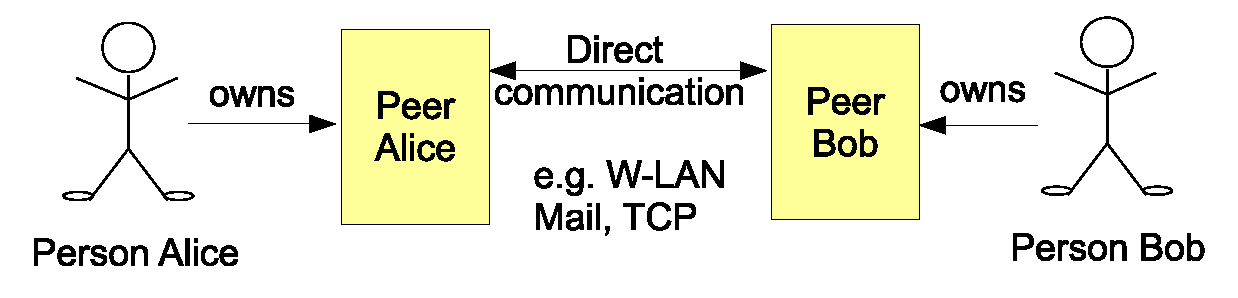
\includegraphics[width=0.60\textwidth]{generalConcept.eps}
\caption{People own peers which can communicate}
\label{fig:generalConcept}
\end{figure}

\section{Communication principles}
The Shark communication protocol is called {\it Knowledge Exchange Protocol (KEP)}. It has just two message types:

\begin{description}
    \item[Expose (interest)]
Owners can define their {\it interests}. One might define that he is interested in {\it cooking, skiing} and {\it Star Trek}\footnote{which was a TV series in the 1990th in the US which the author liked (and still likes) very much.} Another one might be interested in {\it vegetarian cuisine, sports} and {\it science fiction}. 

At the first syntactical glance, both peers don't have anything in common. Sports isn't the same as skiing and vegetarian food isn't just food. A bit more elaborated semantic view can reveal that skiing is a {\it kind of} sport etc., though. 

Shark provides a semantic data model which helps to recognize that both peers have similar interest. This point will be explained later in more detail.

Moreover, a peer can define with whom it is interested in communicating, what time and at which place. But most importantly a peer is able to define if s/he wants to sent or/and receive information to/from a particular peer.

    \item[Insert (knowledge)]
Knowledge is constituted of information. Each information is put into a {\it context}. A context describes aspects of information, namely information topic, issuer, location and time. Peers can exchange such contextualized information at any time. Peers can received knowledge at any time. And they can do with it whatever they like.
\end{description}

KEP is an {\bf asynchronous protocol} which means that a peer doesn't have to wait for a reply. Each peer can send a message whenever it likes, e.g. when meeting another peer. A peer cannot expect a reply: The other peer might not like to answer or the communication channel is broken during communication.

\subsection{Peers meet}
We often use the phrase {\it peers meet}. What does it actually mean?

It is obvious in spontaneous networks: Two peers have met if they can establish a communication channel. Let's make in more concrete and use Bluetooth or W-LAN in ad-hoc mode as an example. Devices look for other devices in their surroundings.
This process is called {\it device discovery}. Once a device is discovered a connection can be established. In conclusion, we can say regarding spontaneous networks that two Shark peers have met if one has discovered the other one.

Meeting is more complicated in non-spontaneous infrastructures. A Shark peer can run on a device which has hardly the chance to discover new peers in its surrounding, e.g. on a desktop computer. This kind of peer will communicate with TCP or e-mail protocols. Those peers won't meet other peers by chance but they can get peer addresses, e.g. an e-mail address of another peer. In non-spontaneous networks we say that two peers have met if at least one is able to create a communication channel to another peer. This is the case if it got its address and can send a message with the matching protocol.

Apparently, it is very useful to mix both variants. It is often useful to provide a peer an address in a fixed infrastructure, e.g. an e-mail address even if it runs on a mobile (smart) phone. The spontaneous and local network is more secure and faster than e.g. e-mail. But communication can be continued of both peers have left communication range of their local network and switch to Internet communication.

Let's have a look at some scenarios.

\subsection{Base scenario}
\label{sec:concepts:baseScenario}
Alice and Bob are two persons each owning a Shark peer which runs on their mobile devices. Both have defined their interests. We make it simple in this scenario:
Both are interested in {\it P2P systems}. 

Alice and Bob have just installed the software and don't know any other peers, but both have created a mailbox for their Shark application and have stored this address within Shark.

Now they switch on their phones and walk around. They can meet in e.g. an ad-hoc W-LAN network. Both peers would now exchange their interests but also their addresses\footnote{We will see later that this behavior can be changed. A peer can also decide to do nothing if it meets another peer. It can also refuse to reveal its addresses or interests at all. It is up to the application logic. It is just a basic scenario.}.

They can now exchange information about {\it P2P systems.} after their peers have found out that both have mutual interests. After leaving, Alice and Bob have learned two things: 

\begin{enumerate}
    \item They have met each other: Alice knows Bobs address and vice versa.
    \item Both have learned each others interests.
\end{enumerate}

Figure \ref{fig:basisscenario} illustrates the concept.

\begin{figure}[t]
\centering
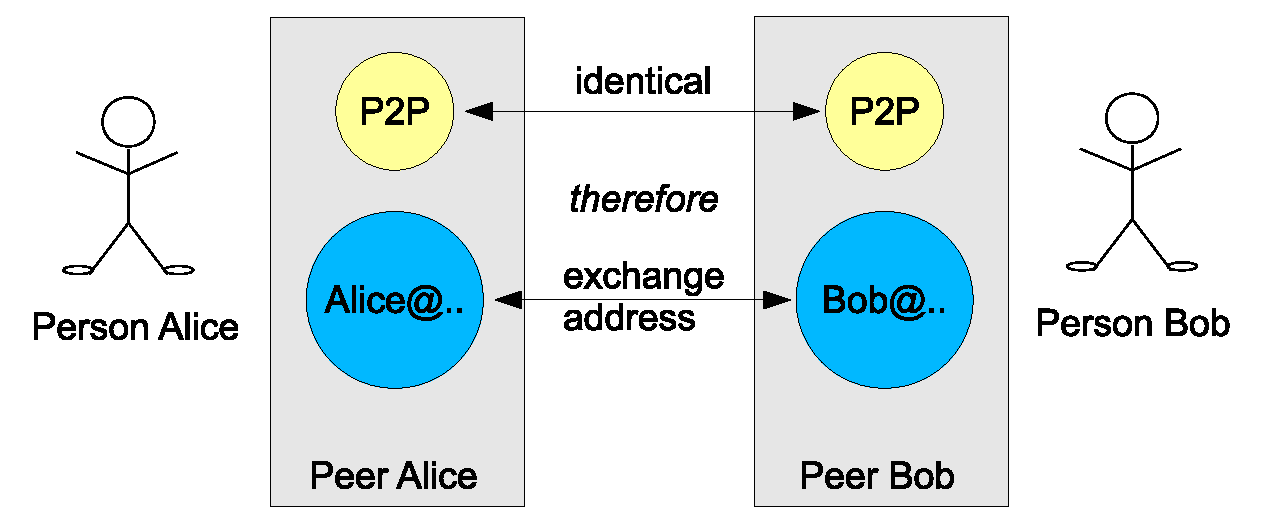
\includegraphics[width=0.60\textwidth]{basisscenario.eps}
\caption{Alice and Bob meet first time}
\label{fig:basisscenario}
\end{figure}

Alice can now send e.g. information about {\it P2P systems} to Bob using e-mail. 
They have met in a spontaneous network, learned about their interests and have also learned a more permanent address which allows them to communicate not only in a spontaneous network.

Programming that basic scenario requires a bit more than a dozen lines of code and will be explained in section \ref{sec:knowledgePorts:StandardKP}.

\subsection{Triangle scenario}
We want to expand the base scenario. Clara may enter the scene. She is also interested in {\it P2P systems} and has also just set up her system.

\begin{figure}[t]
\centering
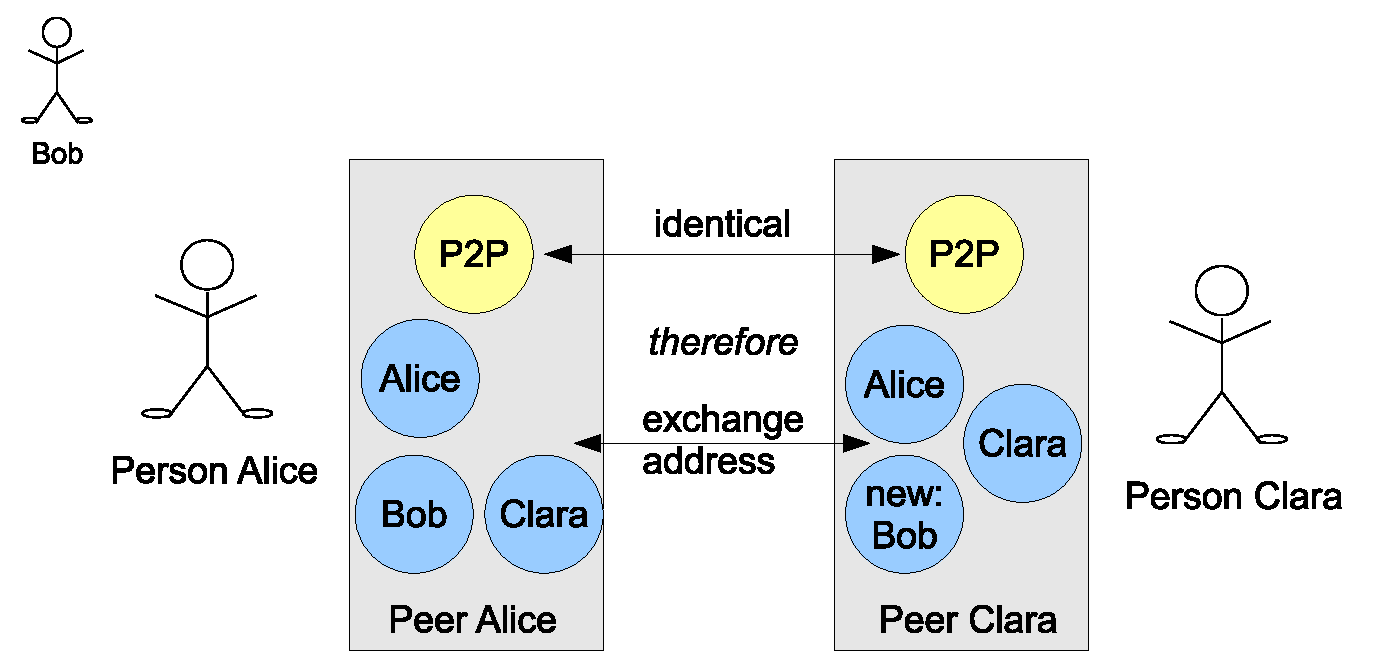
\includegraphics[width=0.60\textwidth]{triangle.eps}
\caption{Alice tell Clara about Bob}
\label{fig:triangle}
\end{figure}

Clara meets her friend Alice. Alice has already met Bob. What happens? First, both perform the base scenario and learn each others interests, addresses and can also exchange information.

Moreover, Alice can\footnote{Can, not must! Any communication behavior can be changed and freely programmed that it fits application needs.} also provide Bobs interest to Clara. In this case, Clara would have {\it met} -- in terms of Shark -- Bob without meeting him personally. 

Now, Clara knows Alice and Bob. Alice knows Bob and Clara and Bob just knows Alice. Maybe Clara sends some information to Bob. In this case he would {\it meet} her as well, see figure \ref{fig:triangle}.

\subsection{Hub scenario}
The triangle scenario leads directly to the hub scenario.

Lets introduce a special peer called {\it Hub}. A Hub has also a permanent address. It has no interests by its own but it is willing to receive any interest from other peers.

Let's imagine, that Hub was just set up and imagine that Alice and Bob didn't meet. Alice could expose her interest in {\it P2P systems} to the Hub. Nothing would happen. As the Hub has no interests by its own and no information to deliver.

Bob could also expose his interest to the Hub. The Hub could now check whether there is a matching interest or not. In this example, it would find Alices interest and would send it to Bob. Bob knows Alice now. He can send information to her or expose his interests.

A Hub is meant to help non-mobile peers to meet. It just stores interests and looks for matching interests. It is a kind of matchmaker. It is important to note that a Hub isn't required any longer if peers have finally met, see figure \ref{fig:hub}.

A Hub should be used as a single entity in a real application. There can be an arbitrary number of hubs, though. A Hub should not be considered to be online permanently.

A Hub is actually a special peer with a very limited application logic. There is a predefined class in the Shark framework that can be used in any application. Thus, any peer can become a Hub, see section \ref{sec:hubkp}. Clara was a hub in the previous triangle scenario.

\begin{figure}[t]
\centering
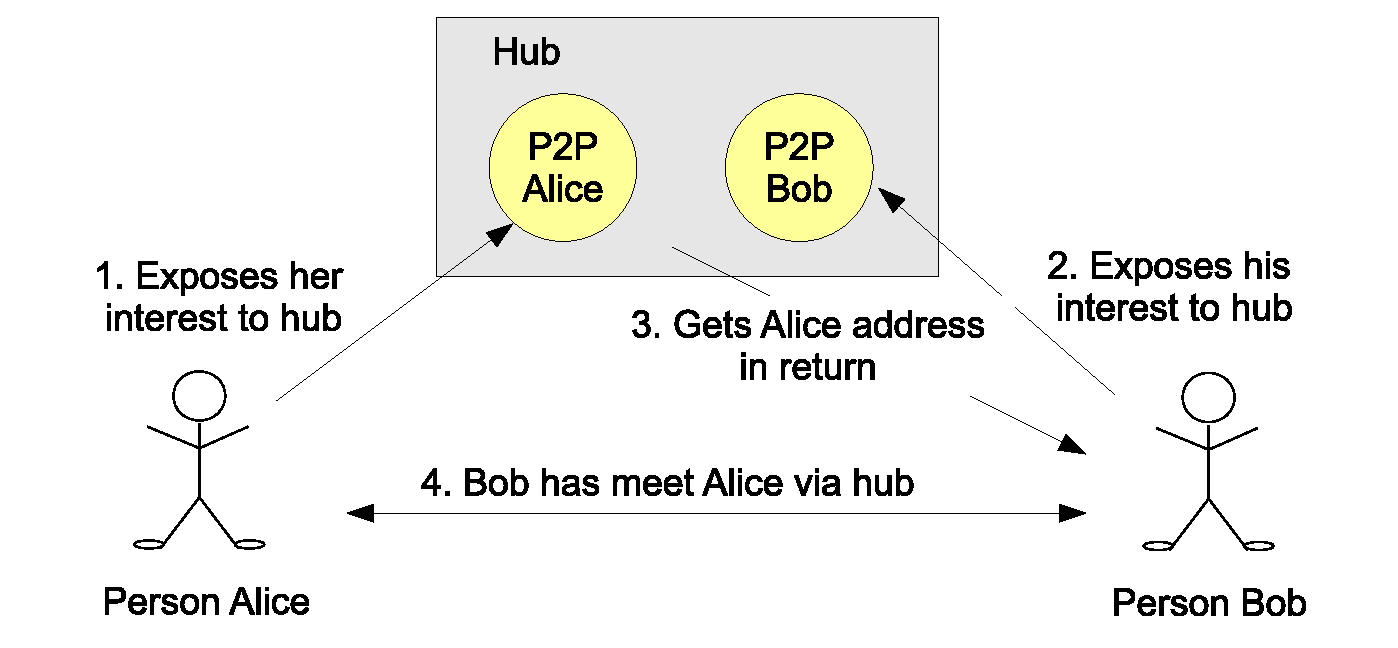
\includegraphics[width=0.60\textwidth]{hub.eps}
\caption{Hub as matchmaker}
\label{fig:hub}
\end{figure}

Of course, interests should be forgotten after a while. The Shark hub implementation allows setting a lifespan for each received interest. The unit is seconds. This underlines the very fact that a hub should not be used as a stable and permanent entity in a fixed infrastructure. Shark applications are P2P applications. As fewer permanent entities exist in a distributed application as more flexible is the overall system.

The Internet is a good example of a reliable system. There are crucial entities but there is no single entity that would switch off the whole network. Web-based applications are different. Just switch off the server (by sabotage, by force (e.g. denial of service attacks), by order of a government, for maintenance, hardware failure or just because also administrators are humans who causes failures) and the whole system is down. A hub shouldn't be used as such a single point of failure and it doesn't has to.

\subsection{Location based scenario}
We can also create a location based service without using GPS and Internet at all. Just take hardware that can establish a spontaneous network and run a peer on it. Let's call this peer {\it Supermarket}. The Supermarket peer can have some product information. It should - of course - be placed into a supermarket.

Let's assume that Alice enters that market. Her peer can establish a connection to the Supermarket peer. Alice should reveal neither her interests nor her address in this scenario. The supermarket on the other hand side should be more verbose and deliver any product information it has.

Alices peer can decide based on her interests which advertisement fits to her interests and which doesn't. That's an automated process. The person Alice wouldn't be aware of any advertisement which is out of her interest.

A supermarket could be replaced by a gallery, a point of (touristic) interest, a fast food shop etc. Such a peer can also be placed near the office door of an elderly professor to submit his lecture notes to interested students who are passing by.

\chapter{Setting up Shark}
The framework comes as a jar file. Add it to your development environment and you are ready for programming semantic P2P systems. 

Latest version can be found on the web page. It has a name like
{\verb|SharkFW 2.8.1|} and can be found there:

{\verb|http://www.sharksystem.net/get_sdk.html|}

Download a code example from 

{\verb|http://www.sharksystem.net/tutorials.html|}, e.g.
the {\it Simple Tag Example}.

Extract and add it to your project. It should compile and run now.

More -- and maybe more current -- information can be found at our web page:
{\tt http://www.sharksystem.net/get\_sdk.html} 

\chapter{Semantic Tags}
The term {\it tag} became quite popular in Web 2.0. The {\it interactive} Web allows users adding comments and/or describing web content. Wikpipedia seems to be the most famous applications in that field.

Brief descriptions are called {\it tags} which are -- in IT terms -- {\it strings}.

This tutorial could be tagged with e.g. {\it Shark} and {\it P2P}.
Tags are well-known in social networks as well. User describe their interests with tags. The author described his interest in Java e.g. with the string ''java''\footnote{on my page on XING}.

Let's have a closer look at a tag, e.g. {\it P2P}. There are some trivial observations:

\begin{itemize}
\item
Tags are usually compared by string comparison. Meaning: {\it p2p} isn't {\it P2P}. Some systems might ignore lower or higher case letters but even so {\it Peer-to-Peer} is different from both.

More sophisticated systems might help to overcome those obstacles. A dictionary can help to find out that two strings have the same meaning.

\item
An ordinary dictionary won't help to find out that {\it bank} and {\it finance institute} can be considered to be the same. There can be different words having the same meaning. They are called {\bf synonyms}. A synonym dictionary can help in this case.

\item
Languages tend to be merged. Apparently, {\it music}, {\it Musik} and {\it La Musica} are not the same string, not the same words and are no synonyms in any language. They depict the same thing but in different languages.

Dictionaries might help in this case. But how many should we use?

\item
It becomes even worse. Have a look at the tag {\it bank}. We already know that it has something to do with finance. It can also be a furniture that helps to relax our legs, though.

Any natural language has {\bf homonyms} which are words which stand for different concepts. Homonyms can only be detected in context. Unfortunately, tags usually don't have a context. A user might just tag a web page with {\it bank}. What can we learn from that? Not that much.

\item
In the previous lecture we learned about Alice and her interest in {\it skiing}.
Bob is interested in {\it sports}. Both words are no homonyms, synonyms, translations and they are correctly spelled. They don't mean the same thing. Nevertheless, they have something in common.

\end{itemize}

We talk about semantics but haven't used the words yet. Semantic describes the meaning of words. What does {\it bank} mean under given circumstances? The meaning of words can be found out in two different ways: Ask the author or make a text analysis.

First approach is most secure but often not feasible. As to be seen, the second approach is more error-prone and requires sophisticated algorithms, some dictionaries and a computer. In general, it is feasible. Computer based algorithms will fail by analyzing a single word like {\it bank}. How should a compute squeeze out author intention when writing those four letters. That's hardly feasible.

Shark doesn't care how to get semantics but how to represent it. There are no algorithms in Shark which helps to figure out the meaning of words or even lengthy documents. Shark deals only with representation of semantics. How can we store known semantics? How can we work with it? And how can we exchange semantics and documents between autonomous peers? That is what Shark is all about.

Shark uses {\it Semantic Tags} to describe semantics of words. Semantic Tags are derived from the ISO standard 13250 Topic Maps, namely the concept {\bf topic}. We won't have a deeper look into that ISO standard in that book. If you'd find some time: Do it. It is well-written, full of wisdom and -- also important -- quite short.

We have to explain just one concept from the standard: {\bf Subject Identifier} are a core concept of Topic Maps as a well as of Shark.

\section{Subject Identifier}
There are things we want to talk about. We can name those things but the naming can be ambiguous. The things are called {\bf subjects} in the Topic Maps ISO standard. Subjects are things in the real world, e.g. a person, a book, a feeling, virtually anything we can talk about.

How do we represent a subject in a computer? The ISO standards uses {\bf topics} for that reason. They represent subjects in a computer system. A topic can have (an arbitrary number of) names.

Topics must describe their semantics. That's done with a {\bf subject identifier}. We don't refer to the definition in the ISO standard but to the (a bit more limited) understanding in Shark:

A subject identifier (SI) is a URI that refers a human readable source that describes the meaning of the semantic tag. The following URL can be used as SI for the tag {\it bank}: http://en.wikipedia.org/wiki/Bank

There is another URL that can also be used:
http://eo.wikipedia.org/wiki/Banko

The later URL refers a web page describing bank (the finance institute) in Esperanto. Both URLs satisfy the requirements for a subject identifier. What URL should be taken?

The answer is pretty simple: Both of course. When defining a semantic tag find and use as much URLs as you can find. Just ensure that all SI really describe the same {\it thing}.

\section{Definition}
Now we can define a semantic tag:

A semantic tag has one (exactly one) name. It has an arbitrary number of subject identifiers. SIs define the meaning of the semantic tag.

Semantic tags can be created without a single subject identifier. Such semantic tags have no explicit meaning. They might have an implicit meaning. The tag author might have had something in his/her mind when creating that tag. That meaning wasn't described either the author didn't know the meaning, hadn't found an appropriate URL or was short in time.

In any case, the computer cannot detect the meaning. The tag can mean anything or nothing, depending on the context. Tags without a single subject identifier are called {\bf any tags}, see also section \ref{sec:AnyST}.

Two semantic tags are defined to be identical if at least one pair of SIs can be found which refers to the same description. Wikipedia is e.g. a very good source for subject identifiers.

Examples:
\begin{itemize}
    \item (bank, (http://en.wikipedia.org/wiki/Bank)) and \\ (bank, (http://en.wikipedia.org/wiki/Bank)) are apparently identical. \\ Names and SIs are the same.

    \item (bank, (http://en.wikipedia.org/wiki/Bank)) and \\ (Bank, (http://en.wikipedia.org/wiki/Bank)) are identical. \\ Name differs slightly but names are not taken into account when comparing tags.

    \item (bank, (http://en.wikipedia.org/wiki/Bank)) and \\ (Financial institute, (http://en.wikipedia.org/wiki/Bank)) are identical. \\ Name differs but SIs are the same (synonyms).

    \item (bank, (http://en.wikipedia.org/wiki/Bank)) and \\ (bank, (http://eo.wikipedia.org/wiki/Bank)) are not identical. \\ Names are the same but each semantic tag has just a single SI and both SIs differ.

    \item (bank, ()) and \\ (bank, (http://eo.wikipedia.org/wiki/Bank)) are not identical. \\ Names are the same but one semantic tag has no defined semantics due to the lack of a SI. Thus, the first tag has the meaning of anything/nothing, the second stands for a bank - for those who understand Esperanto.

    \item (bank, ()) and (P2P, ()) are identical. \\ Names are irrelevant when comparing semantic tags. Both tags have no defined semantics and therefore they are considered to be identical.

    \item (bank, (http://en.wikipedia.org/wiki/Bank)) and \\ (Bank, (http://eo.wikipedia.org/wiki/Bank, \\ http://en.wikipedia.org/wiki/Bank)) are identical. \\ Both tags use http://en.wikipedia.org/wiki/Bank as a subject identifier.

    \item (bank, (http://en.wikipedia.org/wiki/Bank)) and \\ (bank, (http://en.wikipedia.org/wiki/Bank,\_Iran)) are not identical. \\ Names are the same but the first refers to the financial institute whereas the last refers to a city in the south-west of Iran. Bank is homonym in this case. Note, both homonyms can be distinguished.

\end{itemize}

Subject identifiers solve nearly all problems described above except for the last one.

That's a programmers guide and Shark is a framework for P2P applications. Let's
have a look at some simple lines of code.

\begin{verbatim}
String bankEnglSI = "http://en.wikipedia.org/wiki/Bank";

SemanticTag bankTag1 =
    InMemoSharkKB.createInMemoSemanticTag("Bank", bankEnglSI);
\end{verbatim}

First line is simple. We have created string containing a subject identifier explaining the concept bank in English. The second line creates a semantic tag.
We use the {\tt InMemoSharkKB}. This class implements a Shark knowledge base which will be explained later in more details. For now we just need to know that this class also offers a number of static methods to create our semantic structures in computer memory. Thus, the second line of code creates a semantic tag object in memory with the name {\it Bank} and one subject identifier.

Let's expand our example with the following lines:

\begin{verbatim}
String bankEOSI = "http://eo.wikipedia.org/wiki/Bank";

String[] bankSIs = new String[] {bankEnglSI, bankEOSI};

SemanticTag bankTag2 =
  InMemoSharkKB.createInMemoSemanticTag(
      "Financial institute", bankSIs);

if(SharkCSAlgebra.identical(bankTag1, bankTag2)) {
    System.out.println("identical");
} else {
    System.out.println("not identical");
}
\end{verbatim}

We create another SI which refers to a page that explains bank in Esperanto ({\tt bankEOSI}).
Now, we create an array containing both subject identifiers ({\tt bankSIs}).
It might sound somewhat academic but that array has a dedicated meaning.
It means that both subject identifier actually describe the same thing.
No machine can decide that very fact. Just a human being can make such a decision. That decision must be made carefully
which assumes that decision makers are familiar with the given topic and
the languages - bank, English and Esperanto in this case.

Another semantic tag can now be created. Its semantics is described with both subject identifiers ({\tt bankTag2}).

Finally, both semantics tags can be compared. We use class
{\tt SharkCSAlgebra}\footnote{http://www.sharksystem.net/javadoc/current/net/sharkfw/knowledgeBase/SharkCSAlgebra.html}.

We simple check whether both tags {\it mean} the same. In other words:
Do they have same semantics? Run the program and see the answer\footnote{which is {\tt identical}}.

\subsection{Changing Subject Identifier}
Of course, there are circumstances in which users can not define a subject identifier. At least temporary, there can be situations in which a semantic tag doesn't have a SI which means it has no explicitly defined meaning.

The code it pretty simple. Semantics is not.

\begin{verbatim}
SemanticTag noSI =
    InMemoSharkKB.createInMemoSemanticTag(
        "myFirstTag",
        (String) null
    );
\end{verbatim}

Let's sort that mess. First of all, a human has something in mind when s/he talks about anything. Thus, anything has a meaning. The question is if a subject identifier can be found when creating the tag. If yes, the meaning is made explicit. If not, the meaning remains implicit.

Once a subject identifier is defined, the semantic tag has explicitly got a meaning. This meaning cannot be withdrawn - or at least shouldn't be.

This rule has impact on the programming level. Users can change subject identifiers whenever they want to. Shark will and cannot check the content that is referred to by a SI. Thus, Shark cannot check if descriptions have the same meaning. That's up to the user.

Shark simply refuses to remove all subject identifiers if at least one was set: A SI can only be removed if at least another one exists.

We extend out example:
\begin{verbatim}
bankTag2.removeSI(bankEOSI);

System.out.println("removed SI from bankTag2: " +
  L.semanticTag2String(bankTag2));

// try to remove final SI from tag - fails
try {
  bankTag1.removeSI(bankEnglSI);
}
catch(SharkKBException e) {
  System.out.println("failed: " + e.getMessage());
}
\end{verbatim}

Tag {\tt bankTag2} has two SI. One can be removed. Note class {\tt L}.
It is a helper class and mainly used for debugging purposes. It also
offers a simple way to print out e.g. semantic tags.

Removing the only SI from  {\tt bankTag1} fails. The error message explains the
reason. Run the program and watch the results.

SIs can be added. Be careful! All SI of a tag must mean the same.

\begin{verbatim}
bankTag1.addSI(bankEOSI);
System.out.println("bankTag1 after adding: " +
  L.semanticTag2String(bankTag1));
\end{verbatim}

\subsection{Any}
\label{sec:AnyST}
A semantic tag with no subject identifier has no explicit semantics. This tag might have a name but its explicit {\it meaning} is {\bf anything} which can also mean {\bf nothing} in another context.

Such situations should be avoided. But we have to face reality. Sometimes there
is no SI at hand and we have to deal with it. In Shark we say: Each tag with no subject identifier means {\it anything} - it is an {\it any tag}.

{\it Any} is joker tag in Shark. {\it Any} is identical to each other tag.

\subsection{Algorithms}
We have already seen some methods on semantic tags. Have a closer look into the java doc which is available e.g. on the sharksystem.net web
site\footnote{http://www.sharksystem.net/javadoc/current/net/sharkfw/knowledgeBase/SemanticTag.html}.
We want to explain the algorithms beyond the methods.

\subsection{Is Any}
It can be check whether a tag is an any tag.

$isAny(tag): boolean$

The algorithm is trivial. The result is true if either tag is not set ({\tt null} in Java speech) or tag uses the SI {\it http://www.sharksystem.net/psi/anything}.

We have already seen a tag with no subject identifier. That's the other - the explicit definition of an any tag. It should be used very deliberately.

\begin{verbatim}
SemanticTag anyTag =
InMemoSharkKB.createInMemoSemanticTag("anyTag", SharkCS.ANYURL);

if(SharkCSAlgebra.isAny(anyTag)) {
  System.out.println("anyTag is any");
}
\end{verbatim}

Note class {\tt SharkCS} which offers important constants, e.g. the URL
representing the any / nothing meaning.

\subsection{Identical}
We have already calculated if two tags are identical.

$identical(tagA, tagB): boolean$

The algorithm is straightforward:

\begin{enumerate}
    \item
The framework is implemented in Java. Both parameters are objects which reside in computer memory. The first check is whether both Java objects are identical. In this case, both tags are apparently also identical.

\item
It is checked if both tags don't have any subject identifiers. In this case, both tags have no semantics and are identical.

\item
If only one tag doesn't have a subject identifier, it is is checked whether the second one has the semantics of {\it anything} - which can also be explicitly defined - there is a code example later in this section. If so, both tags are identical.

\item
Both tags have a semantics which is not anything at this point. Now, each subject identifier of {\it tagA} is taken and compared to each subject identifier of {\it tagB}. The algorithm stops immediately if a matching pair is found. Both tags are identical in this case.

\item
Both tags are not identical if this point of the algorithm is reached.

\end{enumerate}

\subsection{Merge}
As we have seen, semantic tags can -- and usually are -- defined more than once by different peers in different manners. Two identical peers can be {\it merged}, though. Merging can only be performed with identical semantic tags.

This operation merges one semantic tag with another one. The latter shall be called {\it target} the first {\it merge tag}:

$merge(target, mergeTag): void$

The target can be changed, but the mergeTag remains unchanged in any case.

The algorithm is pretty simple:

\begin{enumerate}
\item
If the target tag has no name, it gets the name of the merge tag. If the target tag has already a name, nothing happens.

\item
All subject identifiers from merge tag are copied to target. SIs are not duplicated: There is at least one SI that already existed in target and merge before merging. Such identical SIs are not duplicated.

\item
Semantic tags can have properties. All properties from merge tag are copied to target tag.
\end{enumerate}

\begin{verbatim}
SharkCSAlgebra.merge(bankTag1, bankTag2);

SharkCSAlgebra.merge(anyTag, bankTag2);
\end{verbatim}

Both methods merge any data from the right tag into the left tag with the described algorithm. Be careful! Shark merges. It does not check whether both tags are identical or not. It is up to programmers will and knowledge.

Apparently, the first line is useful. Both bank tags mean the same and can be merged. The second line is disastrous. It merges bank with any which is nonsense from a semantic point of view. Bank means bank and {\it not} anything. Be careful with what you're doing!

\section{Exercises}

\begin{enumerate}
    \item
Create a semantic tag that represents the city in which you were born. You must find at least one subject identifier.

Write a method {\tt writeST(SemanticTag st)} that prints name and subject identifier of a semantic tag to {\tt System.out}. Check that method with your semantic tag.

\item
Define another semantic tag that defines the city you are currently living in. This tag should have at least one subject identifier different than the one in the previous task.

Check both of your semantic tags on identity.

\item
If both tags are identical, skip this task.

Create another semantic tag that also represents the city where you were born in. Use {\it one} subject identifier that was already used in the first semantic tag and use at least one SI that wasn't used yet.

Both tags should now have a different number of subject identifiers but should be evaluated as identical. Check that.

\item
Merge both identical semantic tags. Print target and merge tag before merging and after merging. Investigate what happened during the process.

\end{enumerate}

\chapter{Derived Semantic Tags}
Semantic Tags describe things in the real world. In academic speech: They are a {\it representation} of a real thing in a computer system.

Anything can be represented with Semantic Tags due to its general concept. Three special types of {\it things} are of higher importance in Shark which are: Peers (persons in most cases), locations and time frames.

A special Semantic Tag type exists for each of them.

\section{Peer Semantic Tags}
A {\it Peer Semantic Tag (PST)} represents a peer. We have already learned that a peer can represent a person, a group of persons or a mixture of both.

Shark only assumes that a peer can communicate with other peers. Thus, a peer can have addresses which can be e-mail addresses, TCP addresses etc. Shark supports e-mail and TCP in version 2.0. Each address can be represented with a string. Each address type starts with a prefix:

\begin{description}
    \item[mail://] indicates that a e-mail address follows. mail://alice@wonderland.net is a valid address in Shark. Note: The prefix {\bf is not} {\tt mailto} which is used in HTML.

A mail address can have an additional parameter: {\it maxLength}. It describes the maximal message length in kilo bytes that fits into the mailbox.

mail://alice@wonderland.net?maxlLength=2048 is a valid address. It describes the fact that must not exceed the length of 2 MByte\footnote{It can also describe that users don't want to receive message larger than the defined length. The given parameter won't be compared to the information given by the mail provider.}.

If no {\it maxLength} is defined, the default value is used, which is defined as one MByte.

    \item[tcp://] indicates that a TCP address follows.
tcp://shark.wonderland.net:7070 is a valid address. A peer can start a TCP server and communicate its address to other peers\footnote{It is highly recommended for any developer to make detailed security considerations before starting a TCP server on their machines. It might not be the best idea to write applications that present an open TCP port to the Internet without any kind of intrusion detection or application firewall.}.

\end{description}

A Peer Semantic Tag simply adds an arbitrary number of (permanent or temporary) addresses to a Semantic Tag. For example a peer named Alice could described with the following PST:

\begin{description}
    \item[Name] Alice.
    \item[Subject Identifier(s)] http://www.sharksystem.net/alice.html
    \item[Address(es)] mail://alice@wonderland.net
\end{description}

It is straighforward and so is the code:

\begin{verbatim}
String aliceSI = "http://www.sharksystem.net/alice.html";

String aliceMail = "mail://alice@wonderland.net";
String aliceTCP = "tcp://shark.wonderland.net:7070";

String[] aliceSIs = new String[] {aliceSI};
String[] aliceAddr = new String[] {aliceMail, aliceTCP};

PeerSemanticTag alice =
  InMemoSharkKB.createInMemoPeerSemanticTag("Alice",
    aliceSIs, aliceAddr);

System.out.println(L.semanticTag2String(alice));
\end{verbatim}

\section{Time Semantic Tags}
Time semantic tags describe a period of time. They are mainly used to describe time frames in which interests or information offerings are valid. Interests and information are discussed later in this book.

Periods can be described by a start and duration. Both values have to be defined with milliseconds.

The following code creates a TST that covers a whole day beginning {\it now}.

\begin{verbatim}
long now = System.currentTimeMillis();

long dayLength = 24 * 60 * 60 * 1000;

TimeSemanticTag time =
    InMemoSharkKB.createInMemoTimeSemanticTag(now, dayLength);

System.out.println(L.semanticTag2String(time));
\end{verbatim}

The length of a day is calculated. Each day has 24 hours with 60 minutes. Each minute has 60 seconds which has 1000 milliseconds.

\section{Spatial Semantic Tags}
Information or information request can be location based. We need means to
describe locations. There is a quite simple data model called {\it simple feature model} which is supported by nearly any spatial data base. That
models is based on simple geometric structure, namely points, lines and polygons even with wholes. Arbitrary geometries can be combined with a collection which is also a geometry.

The {\it well known text (WKT)} defines a string format to define those geometries.

Shark supports WKT. Of course, Shark has to integrate spatial information into it general model. Spatial Semantic Tags (SST) are created for that reason.
SST add a geometry to a semantic tag.

Thus, a SST can be created with name, subject identifier and geometry.
A geometry can be defined with a valid WKT string.

Moreover, geoemtries can also be defined with absolut values.
The following code creates a point with GPS coordinates of a point in Berlin.
Afterwards, a SST is created which has no semantics but a geometry.

\begin{verbatim}
Geometry geom =
  InMemoGeometry.createPoint(52.45747, 13.52669);

SpatialSemanticTag berlinHTW =
  InMemoSharkKB.createInMemoSpatialSemanticTag(geom);

System.out.println(L.semanticTag2String(berlinHTW));
\end{verbatim}

Note, Shark only supports GPS coordinates! More specific, Shark only supports geometries with EPSG code 4326. Shark is - not yet - a spatial database. But it links spatial data with semantics.

\subsection{Summary}
In general, we strongly discourage usage of {\it any} tags. We can weaken that rule for time and spatial tags. Time semantic tags describe a period and
take their identity, their meaning exactly from that definition.
Spatial geometries have already their own meaning. They define an area on earth. That can be sufficient sometimes. Sometime, it might help to add more semantics. It depends on the applications. We come back to that point when we discuss interests.

\subsection{Exercises}
\begin{enumerate}
\item
Describe yourself as peer semantic tag.
\item
Define your lifespan as time semantic tag.
\item
Define your place of birth as spatial semantic tag.
\end{enumerate}

\chapter{Properties}
This will become a brief chapter. We are going to discuss properties. 

Semantic tags as well as other structures in Shark can have properties which are name-value-pairs. Defining a property is simple.

\begin{verbatim}
SemanticTag shark = 
  InMemoSharkKB.createInMemoSemanticTag("Shark", 
     "http://www.sharksystem.net/");

shark.setProperty("propName1", "propValue1");
String value = shark.getProperty("propName1");

\end{verbatim}

We have created a single tag and added a property {\tt propName1}. The last line retrieves the value. This method would produce an failure if no property with that name exists.

Setting an existing property overwrites the old value. Properties can be removed by setting a null value.

\begin{verbatim}
//remove property named propName1
shark.setProperty("propName1", null);
\end{verbatim}

Developers can define whether a property is {\it transferable} or not. What does that mean?

Shark is used to build P2P systems. Thus, e.g. semantic tags are ought to be transmitted from peer to peer including their properties. This default behaviour
can be overwritten by defining a property as non-transferable.

\begin{verbatim}
shark.setProperty("propName2", "propValue2", false);
\end{verbatim}

\section{Usage}
Don't use properties. That provocative rule has a true background. The real rule is: Use properties only if it's really necessary.

Shark has a powerful data model. Especially context points and information are {\bf the} way to store and transmit data and knowledge. Information can be searched. Properties not.

The problem is that properties are easy to understand - even and especially for undergraduates. Don't fall into that trap! Properties can be sweet poison. Whenever information have to be stored, consider first if they can be stored either in semantic tags or in information and context points. Use properties if those options are impossible. Impossible does not mean: 'Well, I haven't found time to read the following chapters and decided to use these property stuff. It sounds familiar.' Impossible means, you had tried hard to do it otherwise and didn't found a useful way.

\section{System properties}
There are also system properties. Here comes the rule: Don't use it! We mean it. 

Don't use it if your are just about writing a Shark application. Only use it if your are about adding features to the framework. Consult the Shark developer team and get deep insights into the framework. Than it might be useful to use system properties. Until you've reached that level of wisdom: Don't use it!

(You may actually find system properties if your are really curious. But never ever change one of these values! Most probably, you will damage your system.)
        

\chapter{Semantic Tag Sets}
Semantic tags can stored together in a set. Each Shark set behaves like Java sets typically do: Tags can be added and removed. 

Tags can have relations. Relations can only be defined by means of tag 
sets. From that structural point of view, Shark offers three kind of sets:

\begin{description}
\item[ST Sets] are also called {\it plain sets}. The just store tags. Tags don't have any additional relation.
\item[Taxonomy] also stores tags. {\tt TXSemanticTags} can be in a hierarchical 
relations, e.g. tag A is {\tt sub} topic of tag B and tag B is {\tt super} topic of A in that case.
\item[SemanticNet] also store tags. {\tt SNSemanticTags} can have arbitrary relations. Relations are usually illustrated by an arc. One tag can refer another tag with a {\tt predicate}\footnote{Yes, this terminology is taken from W3C RDF. The Shark model is far less complex, though.}.
\end{description}

\section{Create, Merge, Add, Remove}
The following code sample creates a plain tag set. A semantic tag is created and removed afterwards.

\begin{verbatim}
STSet plainSet  = InMemoSharkKB.createInMemoSTSet();

SemanticTag berlin = 
   plainSet.createSemanticTag("Berlin", "http://www.berlin.de");

plainSet.removeSemanticTag(berlin);
\end{verbatim}

That's a good point to discuss relationship between knowledge base, sets and 
tags. Tags can either be part of a tag set or exist alone in memory.

There are several knowledge base implementations which will be discussed later in this book. The {\verb|InMemoSharkKB|} exists only in computer memory. All other implementations persist their data on an external medium.

Semantic Tags {\bf cannot} be moved from one set to another. A tag remains in the environment where it was created. A tag that was created remains in memory. A tag that was created in a tag set remains their until its deletion. 

Tags and sets can be {\bf merged}, though. Merging means creating a copy.
Tags can be merged into a set. Sets can be merged into other sets.

Moving a tag from one set two another could be implemented as two step algorithm: First, merge the tag to the target set. Second, remove it from source set. This algorithm behave as moving only if the target set does not contain an {\it identical} tag. This becomes - hopefully - clear when having a look on the merging algorithm:

First, it is looked for
an identical tag inside the set. If there is one, both tags are merged. A copy of the tag is added otherwise. Note: Properties are copied as well, regardless if their are defined to be transferable or not.

Merging tag sets works similar. All tags from the source set are iterated and merged into the target set.

The following code illustrates some examples.

\begin{verbatim}
// create a semantic tag in memory
SemanticTag paris = InMemoSharkKB.createInMemoSemanticTag(
   "Paris", "http://www.paris.fr");

// create stand alone set in memory
STSet plainSet  = InMemoSharkKB.createInMemoSTSet();

// create tag inside tags a tag set
SemanticTag berlin = plainSet.createSemanticTag(
   "Berlin", "http://www.berlin.de");

// merge a tag into a tag set
SemanticTag parisCopy = plainSet.merge(paris);

// create a kb instance
InMemoSharkKB kb = new InMemoSharkKB();

// get the already created set of topics which is still empty 
STSet topicSTSet = kb.getTopicSTSet();

// merge the berlin and paris tag into the knowledge base
topicSTSet.merge(plainSet);
\end{verbatim}

\section{SemanticNet}
Semantic tags can have relations. More precisely, semantic tags can represent things which have relations. Let's have an example.

A tag might describe Germany. Another tag might describe Berlin which is a city in Germany. We'd like to describe that fact.

\begin{figure}[t]
\centering
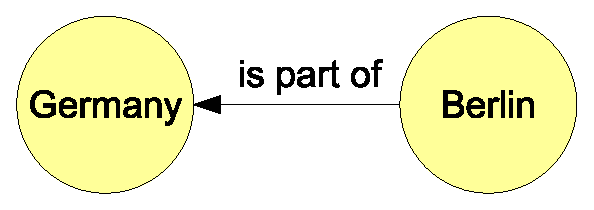
\includegraphics[width=0.40\textwidth]{semanticNet.eps}
\caption{A little semantic net}
\label{fig:semanticNet}
\end{figure}

Tags can refer to another tag by a {\it predicate}. A predicate has two parameters: the referred tag ({\it target} and the predicate name. The origin of the predicate is called {\it source}. 

For our example, the {\it Berlin} tag could refer to the tag {\it Germany} with a predicate named {\it is part of}, see figure \ref{fig:semanticNet}

The following code creates that data structure in memory.

\begin{verbatim}
public class SemanticNetSample {
  public static void main(String args[]) throws SharkKBException {
    SharkKB kb = new InMemoSharkKB();
        
    // handle topics as semantic net
    SemanticNet sn = kb.getTopicsAsSemanticNet();
        
    // describe Germany
    SNSemanticTag germany = sn.createSemanticTag("Germany", 
    "http://en.wikipedia.org/wiki/Germany");
        
    // describe Berlin
    SNSemanticTag berlin = sn.createSemanticTag("Berlin", 
    "http://en.wikipedia.org/wiki/Berlin");
        
    // define a relationname
    String isPartOf = "isPartOf";

    // define berlin to be a part of Germany
    berlin.setPredicate(isPartOf, germany);
        
    /* 
     * what parts of Germany are defined yet?
     */ 
    Enumeration<SNSemanticTag> partsEnum = 
       germany.sourceTags(isPartOf);
        
    // berlin has relations to what tags?
    Enumeration<SNSemanticTag> targetTags = 
       berlin.targetTags(isPartOf);
  }       
}

\end{verbatim}

The first line creates an in-memory knowledge base. The second line
gets a reference to the topic dimension of the knowledge base. Each dimension can be handled differently. It can be handled as plain set, as taxonomy or as semantic net as in this example.

Two tags are created, one representing Germany, another one for Berlin. The string {\it istPartOf} is defined for this application. It is just am arbitrary string! 

The line {\verb|berlin.setPredicate(isPartOf, germany)|} sets the predicate. 

{\verb|germany.sourceTags(isPartOf)|} returns an enumeration of source tags.
Remember, source tags are the start of a predicate. Thus, that method returns any tag the refers to {\tt germany} with the {\tt isPartOf} predicate.

{\verb|berlin.targetTags(isPartOf)|} returns an enumeration of target tags.
In this case, we get all tags to which {\tt berlin} is linked with the {\tt isPartOf} predicate.

Does it sound confusing? On the first glimpse it probably will. It will instantly less frustrating when you have made a little sketch by your own.

To sum up, predicates have the following features and conventions:

\begin{itemize}

\item Each tag can refer to an arbitrary number of other tags. 

\item
Each predicate name can be used in an arbitrary number of predicates.

\item
Referred tags are called {\bf target tags}. The tag that actual refers to another tag is called {\bf source tag} -- it is the source of the predicate.

\item
Predicates can be removed. It doesn't change anything in related tags.

\end{itemize}

\section{Taxonomy}
Taxonomies are special semantic nets. There are just two types of predicates:
{\it super} and {\it sub}. Taxonomies are used if semantic tags can be arranged into a hierarchy of concepts.

Taxonomies have the following features:

\begin{itemize}
    \item 
Tags can be {\it moved under} another tag which means that one tag becomes the sub-tag of another one.

    \item 
Each tag can have an arbitrary number of sub-tags but just one super-tag.

    \item 
A tag without a super-tag is called {\bf root-tag}. A taxonomy has at least one but can have more than one root tag. Our taxonomy is actually a {\it wood}.

    \item 
Tags can be removed. Sub-tags have to be handled in this case. There are two cases: If the deleted tag was a root-tag, all of its sub-tags become root-tags. If the deleted tag was a sub-tag, all of its sub-tags become sub-tags of the super-tag of the deleted tag.

\end{itemize}

Figure \ref{fig:taxonomy} illustrates a little taxonomy that describes the fact that Java and c-Sharp are programming languages.

\begin{figure}[t]
\centering
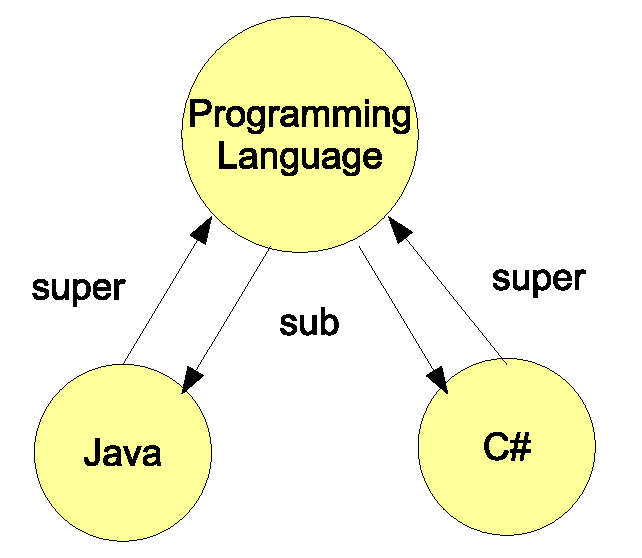
\includegraphics[width=0.40\textwidth]{taxonomy.eps}
\caption{A little taxonomy}
\label{fig:taxonomy}
\end{figure}

The following code creates a data structure representing the same fact.

\begin{verbatim}
public class TaxonomySample {
  public static void main(String args[]) throws SharkKBException {
    SharkKB kb = new InMemoSharkKB();
        
    // we are going to handle topics as taxonomy
    Taxonomy tx = kb.getTopicsAsTaxonomy();
        
    // describe programming languages and java as part of a taxonomy
    TXSemanticTag pl = 
      tx.createTXSemanticTag("PL", 
      "http://en.wikipedia.org/wiki/Programming_language");
    
    TXSemanticTag java = 
      tx.createTXSemanticTag("Java", 
      "http://en.wikipedia.org/wiki/Java_%28programming_language%29");
        
    // move java "under" pl
    java.move(pl);
        
    // describe C#
    TXSemanticTag csharp = 
      tx.createTXSemanticTag("CSharp", 
      "http://en.wikipedia.org/wiki/C_Sharp_%28programming_language%29");
        
    // define c# as sub topic of programming lanugages
    csharp.move(pl);
  }
}
\end{verbatim}

\section{Tag set operations}
Operations on semantic tag sets are actually the heart of the semantic algebra of Shark. Fragmentation and contextualization are basically defined with the tag sets. Later we learn about calculating mutual interests of different peers, extracting information from knowledge bases and assimilating knowledge. Every of those complex operations is based on the following basic operations.

\subsection{Is in}
From a logical perspective, a tag set is a disjunction (OR combination) of its tags. It can be checked whether a tag is in a set or not. Not: {\it is in} {\bf does not} mean that the actual object is in the set. {\bf It does mean} that {\it an identical tag} is in the set.

Tag set offers the {\tt isIn} method. The following code does the same job:

\begin{verbatim}
if(plainSet.getSemanticTag(paris.getSI())) != null) {
  System.out.println("is in");
}
\end{verbatim}

Remember our code from plain sets. A tag {\tt paris} was created to represent the capital of France. Tag identity is made up their subject identifier which can be retrieved with {\tt getSI()}. No, we can try to {\tt getSemanticTag} from {\tt plainSet} which is identical to {\tt paris}. 

This call succeeds if a identical tag of {\tt paris} in in {\tt plainSet}.

It is easier to write {\verb|plainSet.isIn(paris.getSI())|}

\subsection{Is any}
A tag set that only contains tags, that are defined with {\it any semantics}, are said to be an {\it any set} itself.

In other words: A set is an any set if it 

\begin{itemize}
    \item is empty or
\item
all tags have no semantics.
\end{itemize}

In all other cases a tag set is not an {\it any set}. Our Shark algebra helps again:

\begin{verbatim}
boolean isAny = SharkCSAlgebra.isAny(plainSet);
\end{verbatim}

\subsection{Identity}

Tag sets (lets call them A and B) can be identical. That's the case if for every tag in A an identical tag in B can be found and vice versa.

The definition ensures that A is not a sub set of B or vice versa. They are identical. The definition does not ensure that both sets actually contain the same Java objects. Tags can be identical without using identical memory in the computer.

Our algebra can help again:

\begin{verbatim}
boolean isIdentical = SharkCSAlgebra.identical(plainSet, plainSet2);
\end{verbatim}

\subsection{Merge}
A {\bf tag} can be merged into a set. An identical tag can already be in the set. In this case, both tags are merged (see tag merging in a previous section). Otherwise, the a copy of the tag is added to the set. The tag itself won't be changed in any case.

A {\bf set} (called {\it source}) can be merged into another set which is called {\it target set}. Each tag of the source will be merged into the target. Any relations between the tags are copied as well. After merging, the target is usually changed. The source won't be changed.

The following code first merges a single tag into a set. Second, a whole set is merged into another one.

\begin{verbatim}
plainSet.merge(paris);
plainSet.merge(plainSet2);
\end{verbatim}

Merging of sets works also with taxonomies and semantic nets. In this case, all predicates are merged as well. Such merging is a two step operation: First, all tags from the source are merged into the target with the described algorithm. Afterwards, all predicates are merged as well. 

\section{Fragmentation}
Fragmentation is one of the core algorithms in Shark. It is used in many different ways and comes in a number of different versions. We are going to discuss most of them here. It is crucial to understand that method even if it might take a while to understand the concept.

Fragmentation is a powerful tool to find out e.g. if two persons share similar interests. Fragmentation can be compared with a database query but on a semantic level.

\subsection{Plain set fragmentation}
The fragmentation operation creates a sub set from a tag set. The operation has at least two parameters: a {\it source} tag set that will be fragmented and one semantic tag called {\it anchor}. There are some variations. We start with the trivial one.

A plain tag set is just a collection of tags which are assumed to have no relations. A fragmentation is pretty simple:

During the first step, the sources tags are compared with the anchor tag. If there is no identical tag, the result of this operation is an empty tag set.

Otherwise, a tag set is created and the identical tag is merged into the newly created set.

This trivial version of fragmentation has two possible results: An empty set if the anchor is not part of the source or a set with a copy of the identical tag of anchor which is in the source.

Figure \ref{fig:simpleFragmentation} illustrates the concept.

\begin{figure}[t]
\centering
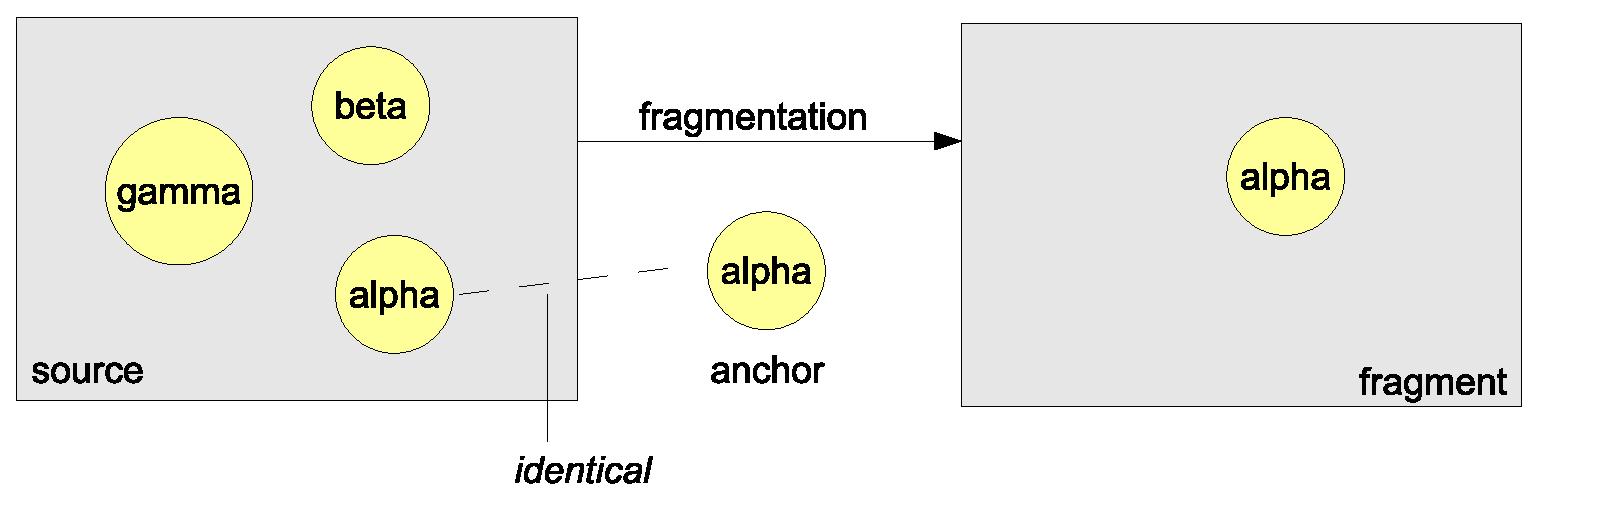
\includegraphics[width=0.60\textwidth]{simpleFragmentation.eps}
\caption{Simple fragmentation}
\label{fig:simpleFragmentation}
\end{figure}

The code constructs the source set, anchor and performs fragmentation.

\begin{verbatim}
STSet source  = InMemoSharkKB.createInMemoSTSet();

source.createSemanticTag("alpha", "http://www.alpha.de");
source.createSemanticTag("beta", "http://www.beta.de");
source.createSemanticTag("gamma", "http://www.gamma.de");

System.out.println("source:" + L.stSet2String(source));

SemanticTag anchor = 
   InMemoSharkKB.createInMemoSemanticTag(
      "alphaAnchor", "http://www.alpha.de");

System.out.println("anchor:" + L.semanticTag2String(anchor));
STSet fragment = source.fragment(anchor);

System.out.println("fragement:" + L.stSet2String(fragment));
\end{verbatim}

Run the code and see what happens. Note, the {\tt L.stSet2String} creates a string representing a set. Class {\tt L} is really useful.

\subsection{Taxonomy fragmentation}
\label{sec:taxonomyFragmentation}
Tags in taxonomies have super- and sub-relations. Therefore, the fragmentation operation has three additional parameters: {\tt depth} (a non-negative integer value) and two boolean values {\tt superAllowed} and {\tt subAllowed}.

\begin{enumerate}
    \item 
The algorithm starts like the trivial variant: The sources tags are checked for a match with the anchor tag. The algorithm stops, if no such tag can be found. 

Otherwise a new taxonomy is created and the identical tag is merged into the new taxonomy. A list of tags is created, let's call it {\it added tags}. The identical tag is stored in this list. The algorithm proceeds with the next step.

    \item 
Depth is decreased. The algorithm stops if the result is below zero.

Otherwise the {\it added tags} list is renamed to {\it current tags} and a new empty {\it added tags} list is created.

The list of {\it current tags} is iterated. The following steps are performed for every entry of the list.

    \item 
If {\tt superAllowed} is false, the next step is taken.

Otherwise, the super-tag of the current tag is taken and merged into the new taxonomy. The predicate is also copied. The super-tag is added to the {\it added tags} list.

    \item 
If {\tt subAllowed} is false, the next step is taken.

Otherwise, each sub-tag of the current tag is merged into the new taxonomy and added to the {\it added tag list}. Predicates are copied as well.

    \item 
After iterating the {\it current tags} list the algorithm continues by decreasing the depth (see above).

\end{enumerate}

Fragmentation is a kind of breadth first search. The parameter {\tt depth} defines the maximal path length from the anchor to another tag. Both logical values define if super- and/or sub-tags should be added to the fragment.

An example should help to fully understand the process. Let's assume we have a taxonomy like shown in figure \ref{fig:taxonomy} and an anchor tag, that is identical to "Tag 2" of the source tag in the picture. With a defined depth of two, {\tt subAllowed} set to {\tt true} and {\tt superAllowed} set to {\tt false}, the resulting tag set would consist of the matching "Tag 2" and all of his sub-tags of the next two layers.

Figure \ref{fig:taxonomyFragmentation} illustrates that process. Source taxonomy describes that programming languages are a part of computer science as well as
the marvelous field of semantic web. Two programming languages are mentioned.

The anchor is programming languages and the fragment is created in both directions: up to more general and down to more specific concepts. The depth is just one. The resulting fragment contains any concept (and any relation) except semantic web. which cannot be reached in one step from programming languages.

\begin{figure}[t]
\centering
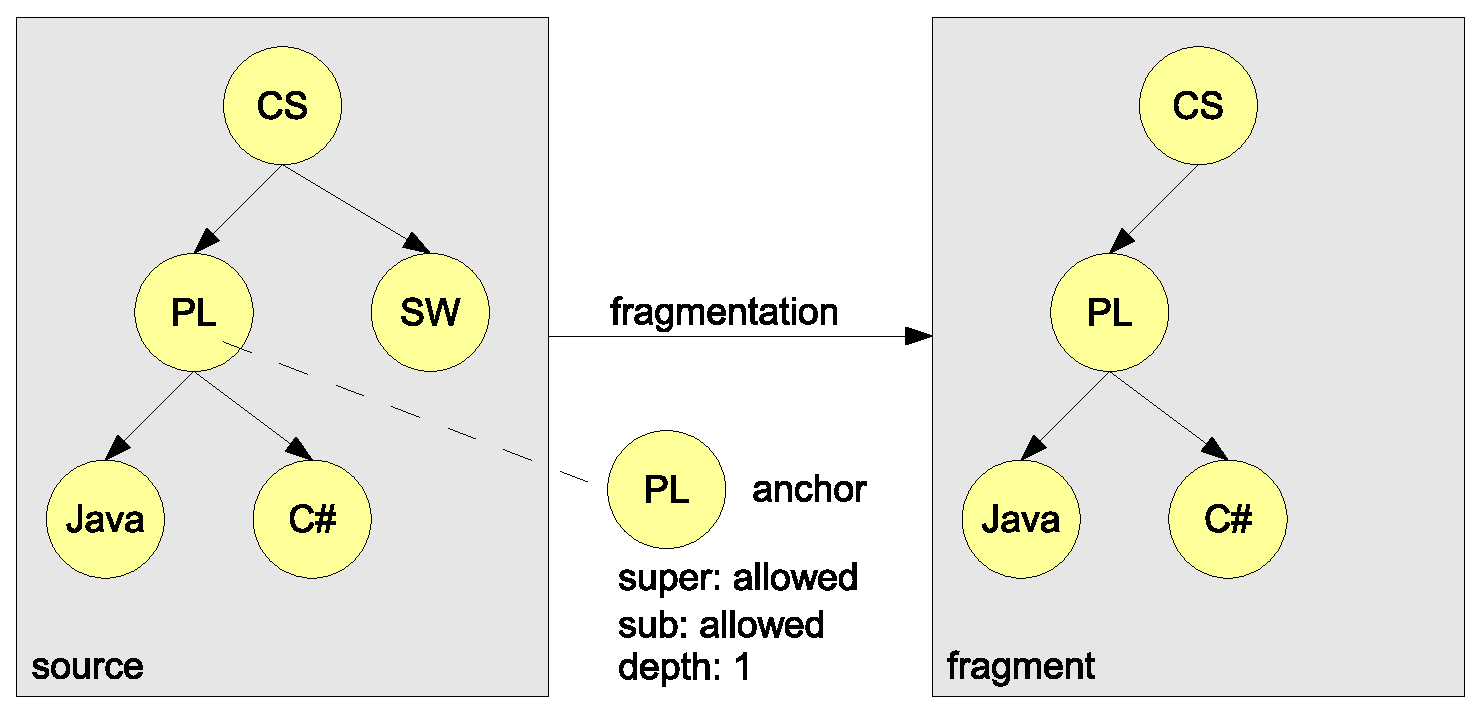
\includegraphics[width=0.60\textwidth]{taxonomyFragmentation.eps}
\caption{Taxonomy fragmentation}
\label{fig:taxonomyFragmentation}
\end{figure}

The following code performs the operation which described in figure \ref{fig:taxonomyFragmentation}.

\begin{verbatim}
Taxonomy txSource = InMemoSharkKB.createInMemoTaxonomy();
TXSemanticTag cs = 
  txSource.createTXSemanticTag("CS", "http://www.cs.de");
TXSemanticTag pl =  
  txSource.createTXSemanticTag("PL", "http://www.pl.de");
TXSemanticTag sw = 
  txSource.createTXSemanticTag("SW", "http://www.sw.de");
TXSemanticTag java = 
  txSource.createTXSemanticTag("Java", "http://www.java.de");
TXSemanticTag csharp =
  txSource.createTXSemanticTag("CSharp", "http://www.csharp.de");

// make pl and sw subtags of cs
pl.move(cs);
sw.move(cs);

// make java and csharp subtags of pl
java.move(pl);
csharp.move(pl);

System.out.println("source:" + L.stSet2String(txSource));

// create anchor tag
SemanticTag anchor = 
  InMemoSharkKB.createInMemoSemanticTag(
    "plAnchor", "http://www.pl.de");

System.out.println("anchor:" + L.semanticTag2String(anchor));

//define fragmentation parameter
boolean superTags = true; // follow super tags
boolean subTags = true; // follow sub tags
int depth = 1; // follow max depth 1

FragmentationParameter fp = 
  new FragmentationParameter(superTags, subTags, depth);

// do fragmentation
STSet fragment = txSource.fragment(anchor, fp);
System.out.println("fragment:" + L.stSet2String(fragment));
\end{verbatim}


\subsection{Semantic net fragmentation}
Fragmentation in semantic networks is the most general variant. It has also a {\tt depth} parameter but instead of two logical values it has two lists of names. They are called {\tt allowedPredicates} and {\tt forbiddenPredicates}. 

Fragmentation in semantic nets is similar to fragmentation in taxonomies except for one variation: The steps three and four in the previous algorithm are replaced with these steps:

All predicates of the current tag are iterated. It is checked for every predicate if it should be used for the fragment. This decision is a little rule-set:

\begin{enumerate}
    \item A predicate is not allowed to follow if its name is in the {\tt forbiddenPredicates} list.

    \item A predicate is not allowed to follow if the {\tt allowedPredicates} list is not empty and the predicate name is not in the list.

\item 
Otherwise the predicate can be used.
\end{enumerate}

Allowed predicates can be followed and all referenced tags are added to the fragment. The previous algorithm is continued with step five.

Figure \ref{fig:semanticNetFragmentation} illustrates a fragmentation with a semantic network. The source contains several relationship between people.

\begin{figure}[t]
\centering
\includegraphics[width=0.60\textwidth]{semanticNetFragmentation.eps}
\caption{Semantic net fragmentation}
\label{fig:semanticNetFragmentation}
\end{figure}

We use Alisha as anchor and allow just the {\it mother} relationship. The depth is set to two. The fragment is just a graph of two concepts: Alisha and her son Ben. Apparently, her sister Carmen isn't reachable by a mother-relation. Therefore, the mother-relationship to Deng isn't part of the fragment.

The following code performs that operation.

\begin{verbatim}

SemanticNet snSource = InMemoSharkKB.createInMemoSemanticNet();
SNSemanticTag alisha, ben, carmen, deng, elias;

alisha = 
  snSource.createSemanticTag("Alisha", "http://www.alisha.de");
ben = 
  snSource.createSemanticTag("Ben", "http://www.ben.de");
carmen = 
  snSource.createSemanticTag("Carmen", "http://www.carmen.de");
deng = 
  snSource.createSemanticTag("Deng", "http://www.deng.de");
elias = 
  snSource.createSemanticTag("Elias", "http://www.elias.de");

// define property names simply as strings
String motherProp = "mother";
String sisterProp = "sister";
String cousinProp = "cousin";
String fatherProp = "father";

// make relations explicit
alisha.setPredicate(sisterProp, carmen);
alisha.setPredicate(motherProp, ben);

carmen.setPredicate(motherProp, deng);

ben.setPredicate(fatherProp, elias);
ben.setPredicate(cousinProp, deng);

System.out.println("source:" + L.stSet2String(snSource));

SemanticTag anchor = 
  InMemoSharkKB.createInMemoSemanticTag(
    "AlishaAnchor", "http://www.alisha.de");

System.out.println("anchor:" + L.semanticTag2String(anchor));

// define allowed properties
Vector<String> allowedProps = new Vector();
allowedProps.add(motherProp);

FragmentationParameter fp = 
    new FragmentationParameter(
            allowedProps, // follow those props
            null, // no forbidden props
            2); // depth == 2

SemanticNet fragment = snSource.fragment(anchor, fp);
System.out.println("fragment:" + L.stSet2String(fragment));
\end{verbatim}

\subsection{Contextualize}
Contextualization is based on fragmentation. There is also a {\it source tag set} of one of our three types. The anchor is no longer a single semantic tag but a semantic tag {\it set}. All other parameters are the same.

{\tt Depth} is used for taxonomies and semantic nets. Both logical values are used for taxonomies and both predicate name lists are used with semantic nets.

The algorithm is short:

\begin{enumerate}

    \item 
An empty tag set is created and called {\it fragment}.
The following step is executed for each tag in the anchor set:

\item
A fragmentation is executed with the source and the current anchor tag and the defined fragmentation parameter. The result is merged into {\it fragment}.

\end{enumerate}
In conclusion, contextualization is a multiple execution of fragmentation.

We use our little family as an example. Figure \ref{fig:semanticnetContextualization} shows the result of a contextualization with the source of figure \ref{fig:semanticNetFragmentation} but Alisha and Carmen as anchor. 

\begin{figure}[t]
\centering
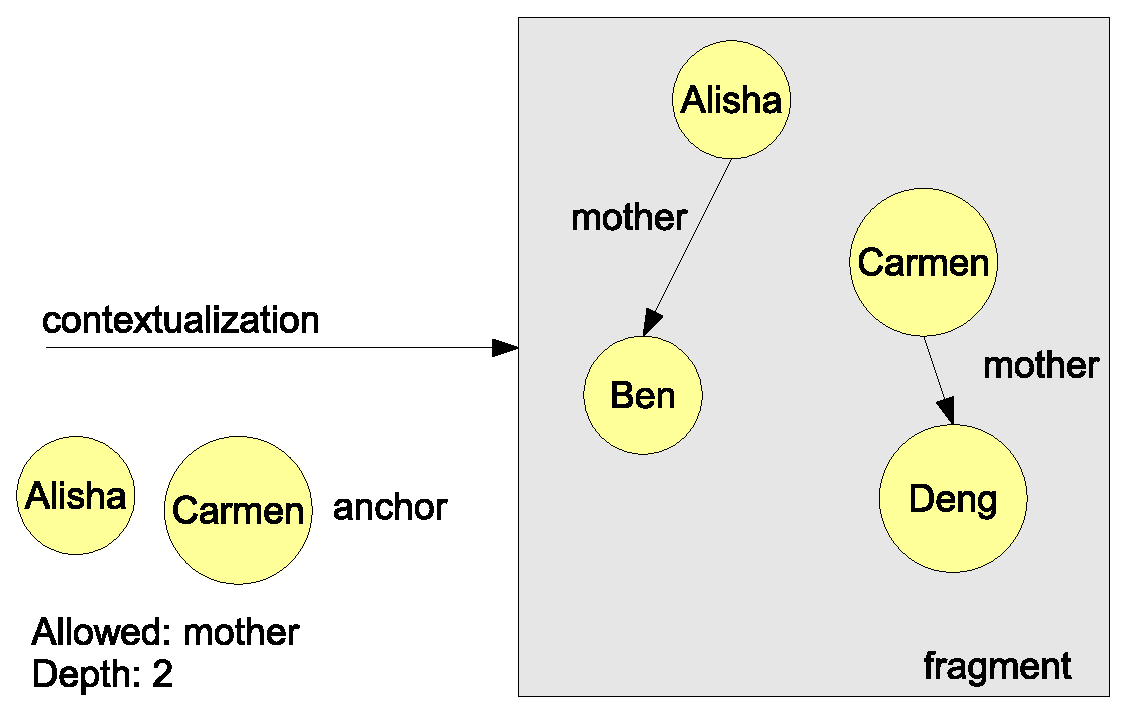
\includegraphics[width=0.60\textwidth]{semanticnetContextualization.eps}
\caption{Semantic net contextualization}
\label{fig:semanticnetContextualization}
\end{figure}

Note: The fragment does not contain relations which are not allowed.
Ben and Deng are part of the fragment. Their relationship is not.
The fact that Carmen is sister of Alisha is also not in the fragment.

For illustration purposes we are going to extend our previous example. 
Let's assume we have still defined Alisha and her family and create an
{\it context} instead of a single anchor:

\begin{verbatim}
STSet context = InMemoSharkKB.createInMemoSTSet();
context.merge(alisha);
context.merge(carmen);

// do contextualization
fragment = snSource.contextualize(context, fp);
System.out.println("after contextualization:" + L.stSet2String(fragment));
\end{verbatim}

Context is an arbitrary tag set. We use the {\tt merge} operation to add tags to the context. Note, merging creates copies of tags in the tag  set. Contextualization differs just in a single parameter from fragmentation.

\section{PeerSNSemanticTag and friends}
We have now discussed Semantic Tags and tag sets. We have learned about special Semantic Tags like Peer Semantic Tags. We have worked with special tag sets, namely taxonomies and semantic nets. 

\begin{figure}[t]
\centering
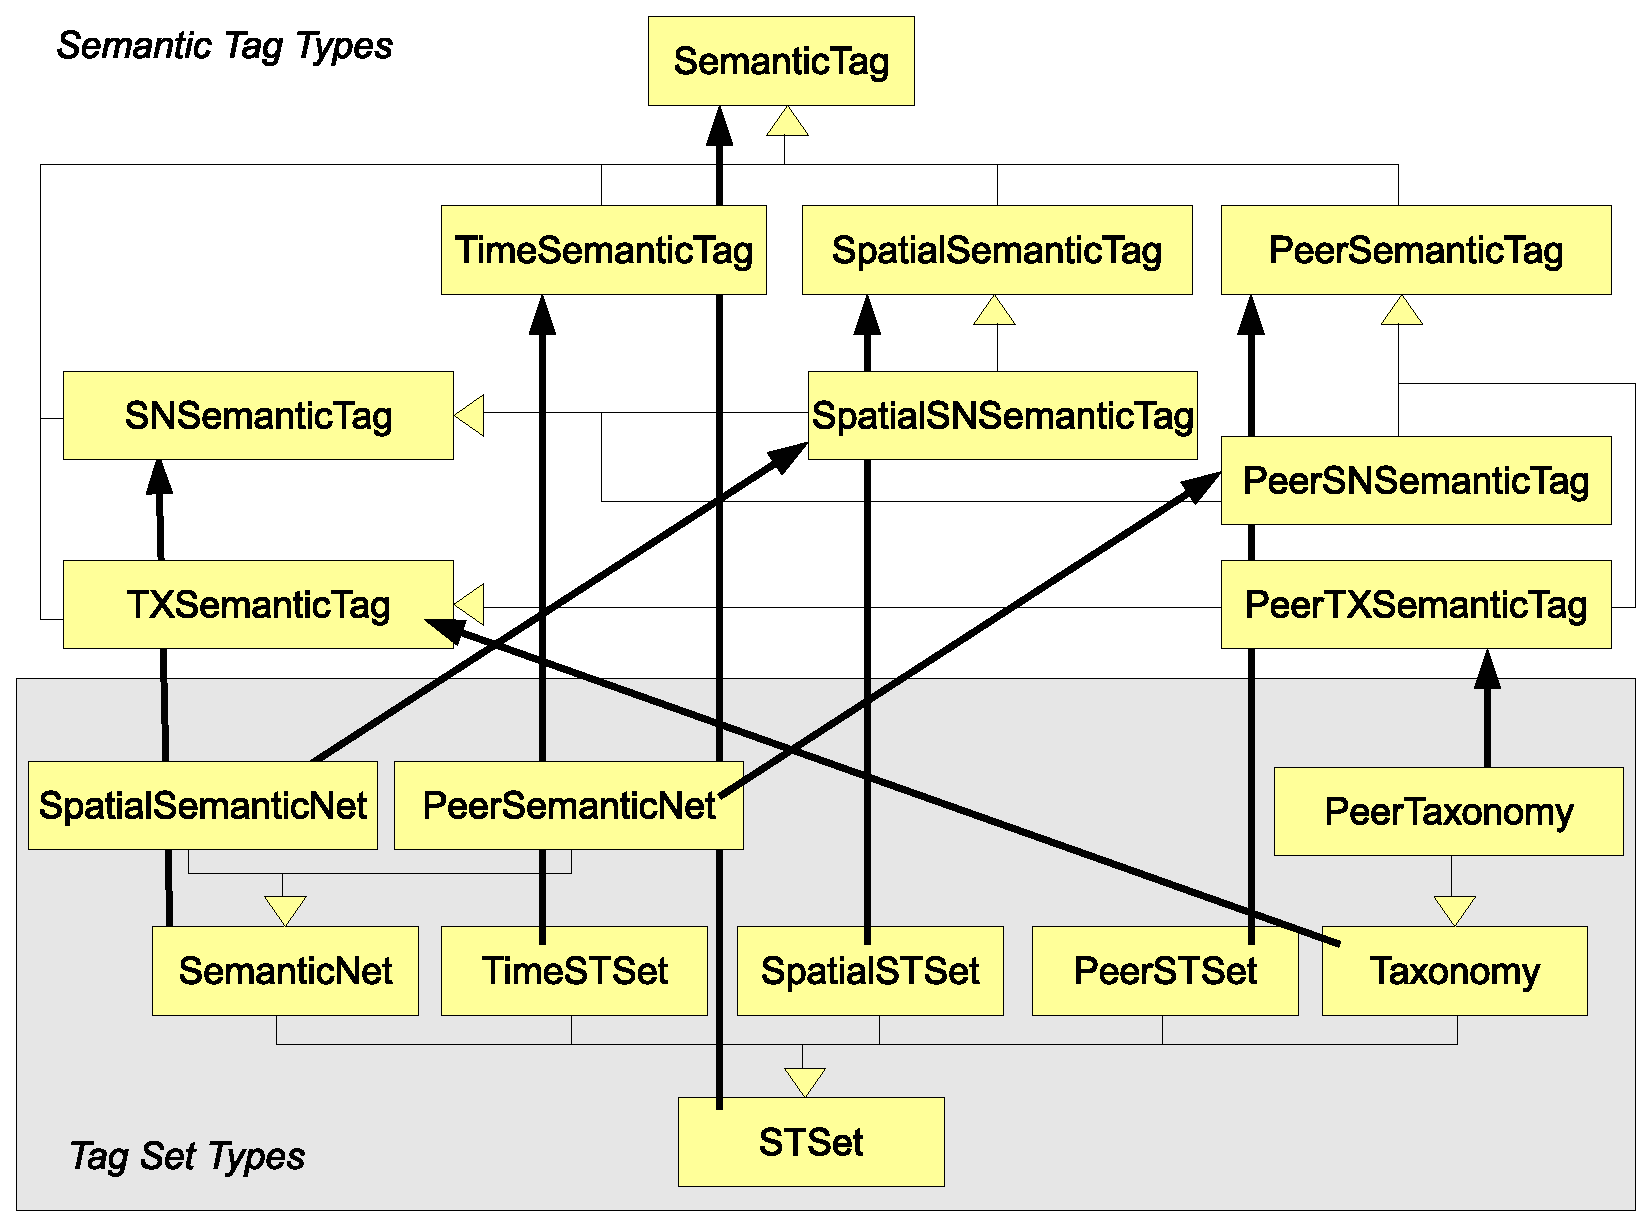
\includegraphics[width=0.80\textwidth]{tagsSetTypes.eps}
\caption{Semantic Tag and tag set types}
\label{fig:tagsSetTypes}
\end{figure}

Apparently, a peer semantic tag {\it is a} semantic tag. That fact can be coded with Java by deriving the {\tt PeerSemanticTag} from {\tt SemanticTag}.  Actually, it is the first line of code in the {\tt PeerSemanticTag} interface:

\begin{verbatim}
public interface PeerSemanticTag extends SemanticTag {..}
\end{verbatim}

There is a similar situation with sets. The most general tag set is {\tt STSet}. Two interfaces extend its abilities: {\tt Taxonomy} and {\tt SemanticNet}:

\begin{verbatim}
public interface SemanticNet extends STSet {..}
public interface Taxonomy extends STSet {..}
\end{verbatim}

Each tag set allows accessing Semantic Tags. For example, one get method declaration is this:

\begin{verbatim}
public SemanticTag getSemanticTag(String si) 
     throws SharkKBException;
\end{verbatim}

There are sets which only contain {\tt PeerSemanticTags}. We have declared a {\tt PeerSTSet} to be type safe in Java. It extends {\tt STSet} and offers a special get method:

\begin{verbatim}
public PeerSemanticTag getSemanticTag(String si) 
     throws SharkKBException;
\end{verbatim}

Note, method name is identical but return type has changed from {\tt SemanticTag} to {\tt PeerSemanticTag}.

Now it becomes a bit complicated due to possible combinations. Just relax and read the following comments calmly. 

There can be a taxonomy that contains Peer Semantic Tags. That set (interface) is declared as {\tt PeerTaxonomy} which extends Taxonomy. It offers a method:

\begin{verbatim}
public PeerTXSemanticTag getSemanticTag(String[] sis) 
     throws SharkKBException;
\end{verbatim}

Have a look at the return type. It is a {\tt PeerTXSemanticTag} which declares a Peer Semantic Tag that is stored in a taxonomy. Such a tag can be handled as Peer Semantic Tag. Addresses can be set for instance. It can also be handled as member of a taxonomy. It can be moved in the tag hierarchy.

There is a number of such combinations, e.g.

\begin{description}
\item[PeerSNSemanticTag] which is a Peer Semantic Tag in a semantic net.
\item[SNSemanticTag] which is general Semantic Tag in a semantic net.
\item[TXSemanticTag] which is general Semantic Tag in a taxonomy.
\item[SpatialSNSemanticTag] which is general Spatial Semantic Tag in a semantic net.
\end{description}

Such types inherit features from two interfaces. Here is an example:
\begin{verbatim}
public interface PeerTXSemanticTag 
     extends TXSemanticTag, PeerSemanticTag {}
\end{verbatim}
No further methods are declared. It is just an aggregation of two existing interfaces, {\tt TXSemanticTag} and {\tt PeerSemanticTag} in this case.


Figures \ref{fig:tagsSetTypes} illustrates that interface hierarchy. The most general semantic tag is to been seen on top the diagram. It has five sub types (spatial, time, peer and taxonomy and semantic net tags). There are three combinations which inherit from two interfaces 
({\tt SpatialSNSemanticTag}, {\tt PeerSNSemanticTag} and 
{\tt PeerSNSemanticTag}.

The tags set hierarchy starts with its most general concept on the bottom ({\tt STSet}. It has two sub types by structure: ({\tt Taxonomy} and {\tt SemanticNet} and three sub types by content types: {\tt PeerSTSet}, {\tt SpatialSTSet} and {\tt TimeSTSet}. Taxonomies and semantic nets can have more specific sub types, namely semantic nets or taxonomies which contain peers ({\tt PeerSemanticNet}, {\tt PeerTaxonomy}). There is also a {\tt SpatialSemanticNet} to describe a network of geographically referenced objects. Other possible combinations like networks of time tags do not exist. There wasn't a need for such combinations until now.

The thick arrows describes a usage relations. A {\tt PeerSemanticNet} e.g. uses (or contains) objects of type {\tt PeerSNSemanticTag}. The most general {\tt STSet} stores {\tt SemanticTag} objects etc.

Why dealing with that mess? Because of types! Type safe programming is professional programming. Thus, peer information have to be stored in a {\tt PeerSTSet} and not in a general {\tt STSet}. In most cases, programmers aren't bothered with choosing the right tags set type. And that is good news. Usually it is already dictated by the knowledge base and its underlying concept of context space which will be described in the next chapter.

\section{Exercises}
\begin{enumerate}
\item 
Change the code from section \ref{sec:taxonomyFragmentation} and let sister relations become part of the fragment.
\item 
\item 

\end{enumerate}

\chapter{Context Space}
\label{sec:contextspace}
\section{Information}
Shark is created to store and exchange information. Information is understood in the same way as in most other content management systems: an arbitrary number of bytes which won't be interpreted by the system.

Shark offers methods to store, find, exchange and delete information. It does not offer means to investigate actual content of information. Shark has features of content management systems. Search capabilities are work just on meta information which are described in this chapter.

Shark is a semantic system. Information are always stored with a description which are defined in the section \ref{section:informationcontext}.

Information can have a structure and can be of a dedicated type. Shark allows using MIME-Types to describe information types. Shark keeps also track of creation time of information.

Lets start with the concepts. Code is presented later in this chapter.

\section{Context Coordinates / Context Point}
\label{section:informationcontext}
Each information can be stored with up to seven types of metadata.

Those types are called {\it dimension} or sometimes {\it facet}. Each dimension is described with a single semantic tag. All seven pieces of metadata together are called {\it context coordinates}.
Now we are going to explain semantics of each dimension.

\begin{description}
    \item[Topic] describes what this information is about. Apparently, a topic is a semantic tag.
    \item[Originator] describes a peer. A peer semantic tag is used. Now, what role does that peer play?

Information is about something that is described by a topic. Tourist information can be about a city. Historical information can be about a historical event etc. That's already defined with the topic aspect and it isn't quite new. That's the very idea of tags in Web 2.0 and the more elaborated Semantic Web. Give users a chance to describe the topic of information. What both Web 2.0 and Semantic Web forget is pretty simple but nevertheless astonishing:
{\it Who} made that description?

Let's have an example:
There is a model in which the earth is orbiting the sun. Centuries ago a scientist claimed that this model would describe our reality. Others called it heresy and burned him.

Who is right? The decision was clear in the  mediaeval times. Sun is orbiting earth. Shark simply ignores this question and allows to put the same information to different topics by remembering who made that classification - who choose the topic:

That's the originator. The peer that declares that this specific information fits to that specific topic. This concept has at least two impacts.

\begin{enumerate}
\item
Information can be stored with different topics by different originators. Shark does not decide what setting is {\it true} or {\it false}. Both originator think they are right.

\item
A peer can put itself into the originator role at any time. It removes the former originator. The peer does not claim to be information creator but it agrees that the chosen topic is appropriate. This step is crucial in Shark because a change of mind happened: the peer (more specific, the human owing that peer) has read and understood something. That process is called {\it assimilation}.
\end{enumerate}

    \item[Peer] Information can be sent to other peers. The peer dimension states who will be the sender in that case.

    \item[Remote Peer] Information can be exchanged with other peers. The remote peer dimension states to whom information can be sent - or from whom information were received.

    \item[Location]
The location aspect defines at which place the peer is willing to communicate. This dimension does {\it not} define a kind of spatial validity of information. Example: Let's imagine location would define Aleppo in Syria. It would {\it not} state that the peer is interested in information {\it about} Aleppo. It would state, that the peer wants to exchange information {\it in} Aleppo.

Topic dimension can be used to describe that information are related to locations. A semantic tag {\it Aleppo} could be used in topic dimension. Moreover, the tag can be used in topic {\it and} location dimension. In that case, peers are interested in exchanging information about Aleppo only in Aleppo. Sounds like a location based tourist guide\footnote{At least, it will hopefully sound like a tourist guide in next future. The author has spent a short but marvelous time in Aleppo and is still very grateful for the generous hospitality. May that civil war end better yesterday than tomorrow as any military conflict. It's a shame.}.

Apparently, location dimension can be used to create location based services.

    \item[Time]
The time dimension defines the time of communication. It does not limit the validity of information. It does describe the time in which a communication can take place.

Thus, a peer could define to exchange information about the ancient Constantinople between 10 a.m. and 4 p.m.

    \item[Direction]
This final dimension describes the direction of information exchange. If a peer wants to deliver information, it would state this aspect to be the {\tt OUT} direction. The value {\tt IN} notes the fact that a peer wants to receive or already has received information. {\tt INOUT} is obviously the combination of both. The {\tt NOTHING} setting describes that the peer doesn't want to exchange information at all.

The final parameter might look a bit strange at the first glance. But it is useful in several cases, e.g.: Peers can store information with Shark. Peers can decide from time to time to hide information or even whole topics from other peers. Therefore they can just set the {\tt NOTHING} direction and no exchange will performed.

\end{description}

That was hard stuff. Let's relax and have a look at some code.

\begin{verbatim}

SemanticTag shark =
  InMemoSharkKB.createInMemoSemanticTag(
         "Shark", "http://www.sharksystem.net");

PeerSemanticTag alice =
    InMemoSharkKB.createInMemoPeerSemanticTag(
            "Alice", // name
            "http://www.sharksystem.net/alice.html", // si
            "mail://alice@wonderland.net"); // address

ContextCoordinates cc = InMemoSharkKB.createInMemoContextCoordinates(
    shark, // topic
    alice, // originator
    alice, // peer
    null, // remote peer: any
    null, // time: any
    null, // location: any
    SharkCS.DIRECTION_OUT); // direction

System.out.println("Coordinates: \n" + L.contextSpace2String(cc));

ContextPoint cp = InMemoSharkKB.createInMemoContextPoint(cc);
Information info = cp.addInformation("Hello Shark");
\end{verbatim}

This code creates coordinates. Just three dimension are declared. Information is about {\it topic Shark} which is created ({\it originator}) and stored ({\it peer}) by Alice. Alice has described no constraints regarding recipients, time and place of an information exchange. She wants to deliver information ({\it direction out}).

A {\tt context point} links context and information together. The final line creates a single string and stores it with its context coordinates. In Shark we say: {\it We put information into a context}.

Context points are created and stored with a {\tt SharkKB}. We mostly use the in-memory implementation for our examples. There are others, see section \ref{sec:sharkkbimplementations}.

\section{Storing and retrieving information}
Data- and knowledge bases are means to store information. A key is required to address information. {\tt ContextCoordinates} are the key in Shark.

Note: We haven't stored our information in a knowledge base in our previous example. We have just created those structures in computer memory but not in a knowledge base. That's done with the following lines which extend the previous code.

\begin{verbatim}
InMemoSharkKB kb = new InMemoSharkKB();

ContextPoint kbCP = kb.createContextPoint(cc);

Information kbInfo =
   kbCP.addInformation(info.getContentAsString());
\end{verbatim}

We create an instance of the in-memory knowledge. Now, we can create a context point {\it in} the knowledge base. Finally, we set up a new information object and initialize it with the string from the previously created information.

We have a knowledge base now. We can retrieve information. The code is trivial:

\begin{verbatim}
ContextPoint kbCP2 = kb.getContextPoint(cc);
\end{verbatim}

There are other and more sophisticated methods of information retrieval. We have to discuss another concept called {\it interest} prior.

\section{Interests}
Our data structures become longer from section to section. We need a more compact representation of context coordinates. Throughout the rest of the book we will write coordinates like this:\\
(shark, alice, alice, any, any, any, out).

We just use the tag names and ignore the -- more important -- subject identifiers.

In the previous section, Alice stored information into a knowledge base and added meta-information. She declared herself as originator and storing peer. She explained that this information is about {\it Shark} and she is willing to exchange it to others.

Let's meet Bob again. Let's say, he is also interested in programming with {\it Shark} but also in diving. In Shark-terms, both are topics. Let's assume that Bob is interested in receiving related information regardless of time, place and sender. We could write in compact form:\\
( (shark, diving), any, bob, any, any, any, in).

Note the two brackets in the topic slot. Bob mentioned two topics he is interested in. We have placed both in the topic dimension. Bob has declared his interest. Therefore he placed himself into the peer dimension. He spared several dimensions because he has no constraints. Bob declares that he only wants to receive something (direction: in).

That's an {\bf interest}. It can be read like a sentence: I'm Bob (peer) and I'm interested in receiving (direction in) information regarding shark and diving (topic) from arbitrary people any time at any place.

\section{Geometrical interpretation}
It's now time to give a geometrical interpretation of that what we have discussed until now. Information are stored with coordinates. Each dimension is described with a single semantic tag. That fits with the definition of Cartesian space: We have seven independent dimensions. A point in that space is described by seven values. We use semantic tags as values.

We call this seven dimensional space a {\bf context space}. Information can be stored in that space. Context space is just a concept. The actual realization of such storage is provided by knowledge bases.

Each person, each peer in Shark has its own context space. Each peer has got its own set of tags and its own set of information. Peers are free to exchange data but they don't have to. Each peer stores its data by its own. There is no need for any centralized data. Shark is a pure P2P system.

What is an interest from a geometrical perspective? An interest can have more than one tag in each dimension. Apparently, it does not define a single point.

Let's come back to our example. Reduce his interest two just three dimensions: topics, peer and remote peer. Imagine a three dimension space,
see \ref{fig:contextspace}.

\begin{figure}[t]
\centering
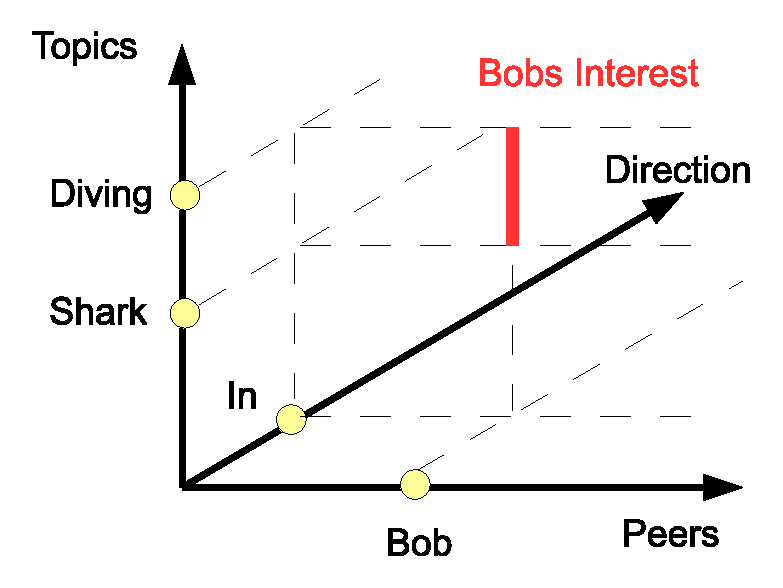
\includegraphics[width=0.60\textwidth]{bobsInterest.eps}
\caption{Bob's Interest}
\label{fig:contextspace}
\end{figure}

Let's have a look at the peer dimension. Bob has defined himself and no other peers. This definition creates a plane in Bobs context space. All point which are not in this plane are not covered by Bobs interest.

Bob has defined two topics. Mathematically, that definition creates two additional planes which subtend our first plane. Two lines are created. Bob has no restrictions in remote peers. We can conclude now: Any point one each of both lines are in Bobs interest.

More abstract but also more accurate: An interest defines a single hyperplane in the seven dimensional context space. An interest describes a point if each dimension is defined by a single tag. Thus, context coordinates can be seen as special interest.

An interest covers the whole context space if each dimension is defined by the any tag. We call it the {\it any interest}.

Note, a point in context space doesn't have necessarily information. A point is just a set of tags defining a context in which information can be stored.

\section{Find information with interests}
Information can be retrieved from a knowledge base by means of interests.
We continue our previous example.

\begin{verbatim}
// create parts of interest
STSet intTopics = InMemoSharkKB.createInMemoSTSet();
PeerSTSet intPeers = InMemoSharkKB.createInMemoPeerSTSet();

// add copy of shark tag
intTopics.merge(shark);
// add diving tag
intTopics.createSemanticTag("Diving", "http://www.diving.de");

intPeers.merge(alice);

// create interest
Interest interest = InMemoSharkKB.createInMemoInterest(
   intTopics, // topics
   null, // don't care originator
   intPeers, // peers
   null, // don't care about remote peers
   null, // don't care about time
   null, // don't care about location
   SharkCS.DIRECTION_OUT); // look for information to be sent

// use it to retrieve information from kb
Enumeration<ContextPoint> cpEnum = kb.getContextPoints(interest);
if(cpEnum != null) {
   System.out.println("found information");
   System.out.println(L.knowledge2String(cpEnum));
}
\end{verbatim}

Interests have seven dimensions. Most of them are sets of semantic tags. In this example we first create two sets. One will contain interesting topics. The other one contains peers. We use 'Shark' and 'diving' as topics and Alice as peer.

We create an interest with our in-memo knowledge base and use it to look for non-empty context points with {\tt getContextPoints()}. An enumeration object is returned if at least one context point can be found with attached information.
We use our logger class {\tt L} to print the results.

The example will find our one and only information. It was found even without explicitly declaring an originator in the interest. It is set to {\tt null} which means {\it any}.

In some circumstances it might be necessary to escape the usage of {\tt null} as {\it any} tag. Sometimes we look for context points in which a dimension is not set. In this case, we can use this code:

\begin{verbatim}
cpEnum = kb.getContextPoints(interest, false);
if(cpEnum != null) {
   System.out.println("found information");
   System.out.println(L.knowledge2String(cpEnum));
} else {
   System.out.println("no information found");
}
\end{verbatim}

We use the variant {\tt getContextPoints(interest, false)}. The second parameter is set to false. This prevents the knowledge base from interpreting undefined dimensions as {\it any tags}. This version looks for context points with unset dimensions in originator, time and location dimension.

This code will produce the output {\tt no information found}.

Note, {\tt getContextPoints(i, true)} is identical to {\tt getContextPoints(i)}.

\subsection{Any tags in interests}
We want to discuss the use of {\it any} tags in interests in more in detail. You can skip that section during first reading. But come back later.

Semantic tags without an explicit meaning are called {\it any} tags in Shark.
We could already see, that coordinates can have an {\it any} tag. Each dimension has -- per definition -- an {\it any} tag. An exception is the direction.

Thus, {\it any} in context coordinates are interpreted as {\it don't know} rather than {\it anything}. Why is that? Authors create coordinates. They know their content. They will hardly state that information fit to any thinkable topic in the world. More likely, they haven't found an appropriate subject identifier.

The problem arises when facing the interests. What is meant if a user declares {\it any} e.g. in topic dimension? From a technical point of view, it could have two meanings:
\begin{enumerate}
    \item The user is interested in information which has no defined topic. The user is not interested in any information with a declared topic.
\item
The user has no constraints in topics.
\end{enumerate}

We have chosen the last interpretation\footnote{And we have already seen that developers can change that decision. There are two variants of {\tt getContextPoints}, see previous section.} as default. Thus, an {\it any tag} in interests declares that dimension to be free of constraints. Anything would fit.

In conclusion, the most general interest is the following one:

(Any, Any, Any, Any, Any, Any, INOUT).

It could be translated in: A peer that doesn't reveal its identity is interested in sending and receiving information about arbitrary topics. It has no constraints on communication partners, locations and time.

This interest isn't as useless as it might look at the first glance. We come back to the point when we talk about mutual interests.

Let's have a look at this interest:

(Tourist information, Any, Any, Any, Berlin, Any, IN).

This interest can be described as: A peer that doesn't reveal its identity wants to receive tourist information in Berlin. It has no further constraints. Looks like a location based service.

Or this one:

(Any, Any, Bob, Alice, Any, Any, INOUT).

Bob is interested in sharing anything with Alice.

\section{Contextualization}
Now we have reached the very core of the Shark data model and even the Shark concept. Shark is about storing information with context and it is about exchanging information.

Information exchange shall be based on {\it mutual interests}. Now we explain how mutual interests can be {\it calculated}. Let's do it with an example first and let's come back to Alice and Bob.

We have already seen that Alice had stored information about Shark and is willing to share it. She stored her information with a knowledge base and used those coordinates which can also be seen and used as interest.\\
(Shark, Alice, Alice, Any, Any, Any, OUT)\\
She (Alice) offers something about Shark to anybody, anywhere and anytime.

A P2P system needs to be at least one other peer. That's Bob. He might be interested in exchange of anything which is of any interest by Alice. Such interest can be described.\\
(Any, Any, Bob, Alice, Any, Any, INOUT).

Note the last dimension {\tt inout}. He wants to send but also receive  information. Lets have a look on a fresh code example that firstly creates both interests.

\begin{verbatim}
// create alice interest
STSet aliceTopics = InMemoSharkKB.createInMemoSTSet();
aliceTopics.createSemanticTag( // create topic shark
   "Shark", // name
   "http://www.sharksystem.net"); // si

// create peer alice
PeerSemanticTag alice = InMemoSharkKB.createInMemoPeerSemanticTag(
            "Alice", // name
            "http://www.sharksystem.net/alice.html", // si
            "mail://alice@wonderland.net"); // address

// create peer tag set
PeerSTSet alicePeers = InMemoSharkKB.createInMemoPeerSTSet();
alicePeers.merge(alice);

// create interest for alice
Interest aliceInterest = InMemoSharkKB.createInMemoInterest(
   aliceTopics, // her topics: shark
   alice, // she offers her information
   alicePeers, // stored in her knowledge base
   null, null, null, // don't care about time, place, remote peers
   SharkCS.DIRECTION_OUT); // offers information

// debugging: print it out.
System.out.println("Alice interest:\n " +
    L.contextSpace2String(aliceInterest));

// let's do it with bob as well
PeerSTSet bobPeers = InMemoSharkKB.createInMemoPeerSTSet();
bobPeers.createPeerSemanticTag("Bob", // name
            "http://www.sharksystem.net/bob.html", // si
            "mail://bob@wonderland.net"); // address

PeerSTSet bobRemotePeers = InMemoSharkKB.createInMemoPeerSTSet();
bobRemotePeers.merge(alice); // wants to talk with Alice only

Interest bobInterest = InMemoSharkKB.createInMemoInterest(
   null, null, // topic and originator irrelevant
   bobPeers, // that's bob
   bobRemotePeers, // only alice
   null, null, // don't care about time and place
   SharkCS.DIRECTION_INOUT); // sending, receiving

// debugging: print it out
System.out.println("Bob interest:\n " +
    L.contextSpace2String(bobInterest));
\end{verbatim}

Interests are defined by peers. Interests can be sent. Let's assume that Alice has received Bobs interest. For us it is very simple to find the mutual interest. If Bob wants to share anything with Alice and Alice offers information about java to anybody it is obvious: Both have the interest, that Alice sends information about Java to Bob anywhere and anytime.

(Shark, Alice, Alice, Bob, Any, Any, OUT)

Let's have a closer look at the calculation: Bob had no constraints about the topic. Alice did: The intersection of both is Shark. Bob had no constraints regarding originator. Alice did. The intersection is Alice.

Bob has introduced himself as Bob in peer dimension. So did Alice. She introduced herself as Alice. Apparently, Alice should not try to find out if both  {\it peer} dimensions fit. She should try to find out if peer in received interest fits to her constraints about remote peers - and vice versa.

Alice had no constraints about remote peers, Bob only wants to talk with Alice. The intersection is Bob. Alice is making that calculation and Bob is the remote peer.

Bob has constraints about his remote peers: He only wants to talk with Alice. Alice has revealed her identity - that fits. Alice is put into the peer dimension.

Both peers have no constraints in location and time. There are no constraints in the mutual interests either. Bob wants to communicate in both directions. Alice only wants to send.

This sound complicated and actually it is. The good new is - Shark makes those calculations for you:

\begin{verbatim}
// zero fp: don't follow any relation. depth = 0
FragmentationParameter fp = FragmentationParameter.getZeroFP();

//use that fp for each dimension
FragmentationParameter[] fps = new
   FragmentationParameter[SharkCS.MAXDIMENSIONS];

for(int d = 0; d < SharkCS.MAXDIMENSIONS; d++) {
   fps[d] = fp;
}

// calculate mutual interest
Interest mutualInterest = SharkCSAlgebra.contextualize(
   bobInterest, // source - the received interest
   aliceInterest, // context - the local interest
   fps);

// watch the result
System.out.println("Alice calculates: Bob / Alice:\n " +
    L.contextSpace2String(mutualInterest));

\end{verbatim}

Imagine, Bob would receive Alice's interest. He could do the same calculation and would come to that result:

(Java, Alice, Bob, Alice, Any, Any, IN)

That result differs in three points: peer, remote peer and direction. And that's only logical. We are on Bobs side now. Bob puts himself into the peer dimension and Alice in the remote peer slot of course. He also learnt that Alice only wants to send something, so he changed the direction to IN.

We extends our program with those lines:
\begin{verbatim}
mutualInterest = SharkCSAlgebra.contextualize(
   aliceInterest, // source - received interest
   bobInterest, // context - local interest
   fps);

System.out.println("Bob calculates: Alice / Bob:\n " +
   L.contextSpace2String(mutualInterest));
\end{verbatim}

Both mutual interests describe a potential information exchange. Both mutual interests differ because they describe the same exchange from different perspectives.

Bob describes Alice as {\it remote peer} and vice versa. Alice describes an interest in {\it sending} information. This fits to Bob because he wants also to {\it receive} information. Once an interest is received it has to be translated into the recipient peers perspective.

We have used our algebra class {\tt SharkCSAlgebra} for our calculation. Applying {\tt contextualize} on {\tt interest} automatically makes the translation of perspective. The method takes three parameters. First is a {\it source} which is meant to be the received interest. Second parameter is the {\it context} which is meant to be the interest created by the receiving peer.

The fragmentation parameter are used for those calculations. The algorithm is explained in detail in next sub section.

Does it sound complicated even irritating? Don't panic! The good news is that most applications don't have to deal with those details. Everything is already implemented and there are already predefined and implemented classes that perform the information exchange that fits to a huge number of applications (namely {\tt StandardKP}).

Have a look on the algorithm if you like. It is not necessary when first reading this book. Read it if you run into problems in your applications.

\subsubsection{Algorithm}
The algorithm explanation is a brief one compared to the motivation. We already know contextualisation in semantic tag sets. The context space contextualisation algorithm works as described below.

\begin{enumerate}
    \item The Algorithm has two parameter: Source and context. Both are context spaces. A third context space will be the result -- we call it fragment.
\item The topic dimension in the fragment is created by means of a contextualisation of two semantic tag sets. The source set is the topic dimension of source and the context set is the topic dimension of the context.
\item The same operation is made with location and time. Source location and time is contextualised with context location and time.
\item The sources originator is contextualised with the contexts originator.
\item
The fragment peer dimension is the result of the contextualisation of the sources remote peer dimension with the contexts peer dimension.
\item
The fragments remote peer dimension is the result of the contextualisation of the sources peer dimension with the contexts remote peer dimension.
\item
The contextualisation of the direction differs from the calculations above and is explained in table \ref{tab:directionCalculation}
\end{enumerate}

\begin{table}[t]
\centering
\begin{tabular}{|c|c|c|}
\hline
Source & Context & Fragment \\
\hline
INOUT & INOUT & INOUT \\
\hline
INOUT & OUT & OUT \\
\hline
INOUT & IN & IN \\
\hline
OUT & INOUT & NON \\
\hline
OUT & OUT & NON \\
\hline
OUT & IN & IN \\
\hline
IN & INOUT & OUT \\
\hline
IN & OUT & OUT \\
\hline
IN & IN & NON \\
\hline
NON & * & NON \\
\hline
* & NON & NON \\
\hline
\end{tabular}
\caption{Direction contextualisation}
\label{tab:directionCalculation}
\end{table}

\section{Other operations}

\subsection{Is in}
The context space describes a sub space. A point can be in the sub space or not.
There is a method that checks whether a point described by context coordinates is within or outside a sub space.

The actual algorithm is straightforward: Most of each context space dimension is described with a set of semantic tags. Each possible combination of coordinates is created. The point is in the context space if one combination fits with the given coordinates.

Let's have an example. We choose just two dimensions to shorten the description.

Lets have a two dimensional space constituted by topic and peer. Lets define a point with the dimension ({\it Java}, {\it Alice}). Lets define a context space:
({\it (Java, Skiing), (Alice, Bob)}). Is the point inside the context space?

The figure \ref{fig:csIsIn} shows the context space and the point (Java, Alice):

We create any possible point inside the context space which are four in our example:\\
{\it (Java, Alice)}\\
{\it (Java, Bob)}\\
{\it (Skiing, Alice)}\\
{\it (Skiing, Bob)}\\

Those four points are the whole context space. Just four points -- nothing more. It is a discrete space -- there is nothing {\it between} Alice and Bob or Java and Skiing. Apparently, the point ({\it Java}, {\it Alice}) is part of the context space.

\begin{figure}[t]
\centering
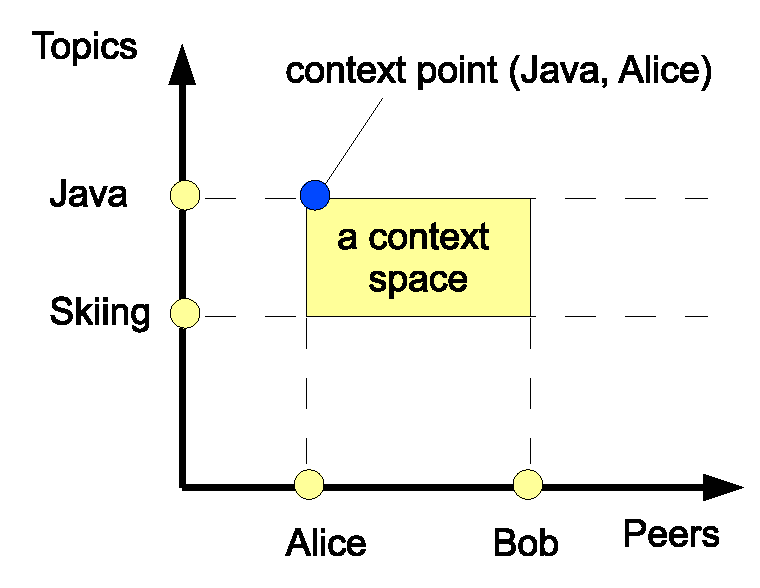
\includegraphics[width=0.60\textwidth]{insideAContextSpace.eps}
\caption{Inside a Context Space}
\label{fig:csIsIn}
\end{figure}

The following code creates an interest, coordinates and performs the test.

\begin{verbatim}

SemanticTag skiing =
   InMemoSharkKB.createInMemoSemanticTag(
         "Skiing", "http://www.skiing.de");

SemanticTag java = InMemoSharkKB.createInMemoSemanticTag(
         "Java", "http://www.java.de");

PeerSemanticTag alice =
   InMemoSharkKB.createInMemoPeerSemanticTag(
      "Alice", // name
      "http://www.sharksystem.net/alice.html", // si
      "mail://alice@wonderland.net"); // address

PeerSemanticTag bob =
   InMemoSharkKB.createInMemoPeerSemanticTag(
     "Bob", // name
     "http://www.sharksystem.net/bob.html", // si
     "mail://bob@wonderland.net"); // address

// create interest (context space)
STSet topics = InMemoSharkKB.createInMemoSTSet();
topics.merge(skiing);
topics.merge(java);

PeerSTSet peers = InMemoSharkKB.createInMemoPeerSTSet();
peers.merge(alice);
peers.merge(bob);

Interest interest = InMemoSharkKB.createInMemoInterest(
   topics, null, peers, null, null, null,
   SharkCS.DIRECTION_INOUT);

System.out.println("interest:\n " +
    L.contextSpace2String(interest));

// create coordinates
ContextCoordinates cc =
   InMemoSharkKB.createInMemoContextCoordinates(
      java, null, alice, null, null, null,
      SharkCS.DIRECTION_INOUT);

System.out.println("CC:\n" + L.contextSpace2String(cc));

if(SharkCSAlgebra.isIn(interest, cc)) {
   System.out.println("is in");
} else {
   System.out.println("is in");
}
\end{verbatim}

\subsection{Identical}
Two context spaces are defined to be identical if both comprises the same points.
We could also say that each point of context A must by {\it in} context B and vice versa. We could also say that all context space dimensions must be identical. That method is simple and so is the code. We extend the previous code.

\begin{verbatim}
if(!SharkCSAlgebra.identical(interest, cc)) {
   System.out.println("Not identical");
}
\end{verbatim}

\section{Context Space interfaces}
Figure \ref{fig:contextSpaceHierarchy} illustrates most important interfaces which make up context space in Shark.

{\tt ContextSpace} just defines the basic fact that a context space is made up by dimensions. {\tt SharkCS} defines number and names of dimensions and some basic methods and important constants. What is {\tt ContextSpace} good for?

It is a heritage and a reminder. There is a more generic theory on context space explained in my PhD. Context spaces is a general concept for independent and co-operating knowledge bases. The number of dimensions is irrelevant for the more general concept. Those, there could be implementations that don't use seven dimensions but an arbitrary other number of dimensions and dimension types.

{\tt SharkCS} describes the Shark context space. It makes clear, that Shark uses seven dimensions with the defined semantics. {\tt SharkCSAlgebra} implements all algorithms for this seven dimensional incarnation. Some classes also offer methods like {\tt contextualization} and {\tt fragmentation}. Finally, any of those methods use this central class. We suggest to use the algebra class whenever possible.

{\tt ContextCoordinates} and {\tt Interests} are derived from {\tt SharkCS} and define point and hyperplane in the context space.

\begin{figure}[t]
\centering
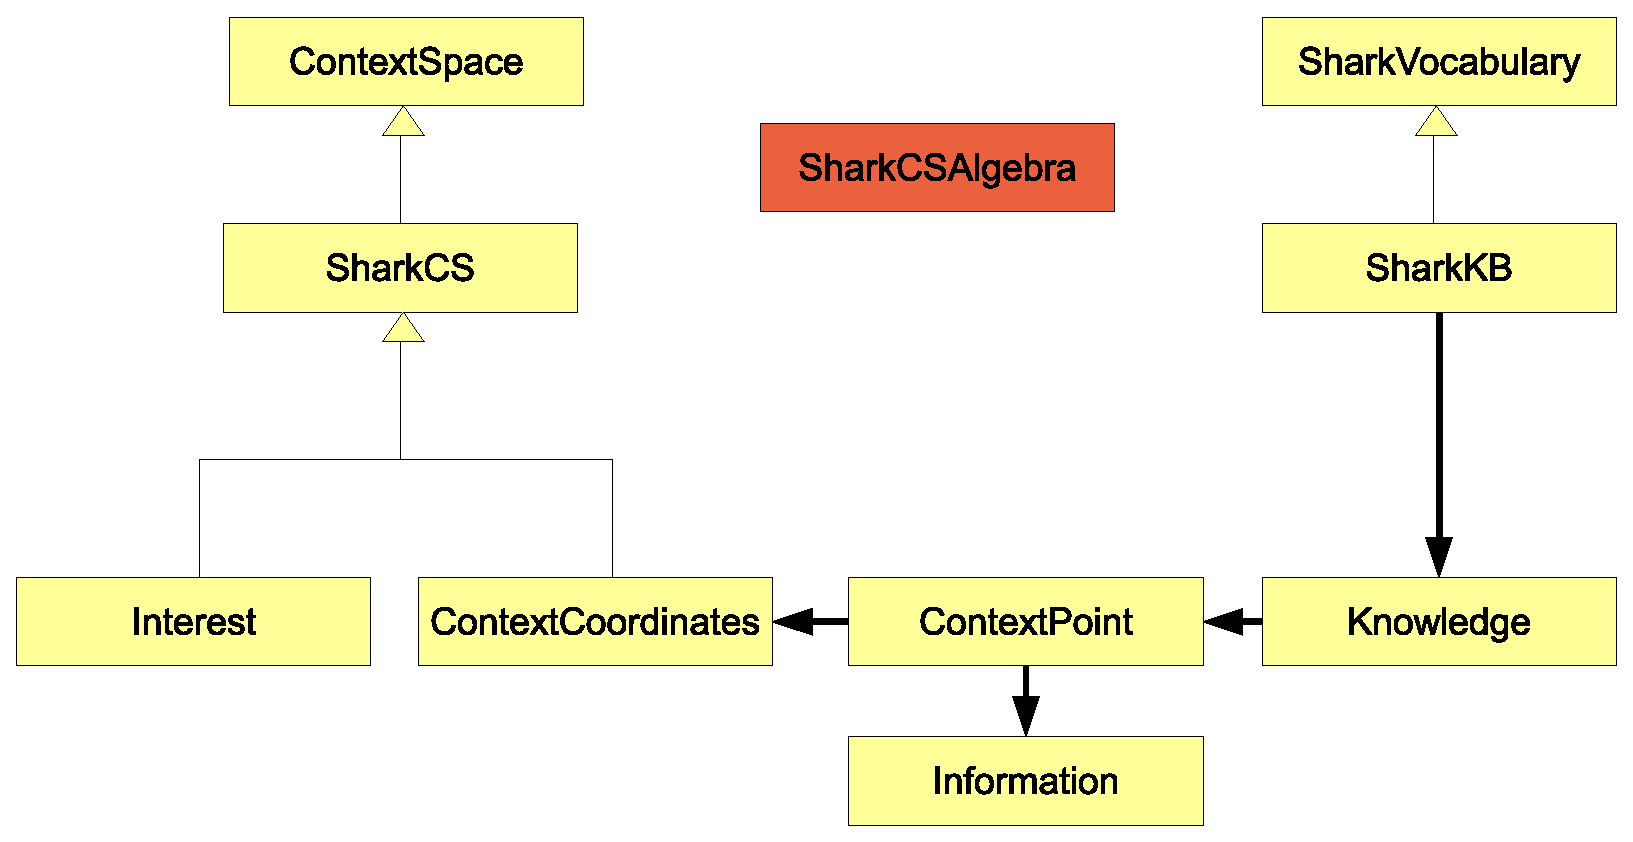
\includegraphics[width=0.90\textwidth]{CSInterfaces.eps}
\caption{Most relevant Context Space Classes and Interfaces}
\label{fig:contextSpaceHierarchy}
\end{figure}

All those interfaces are implemented with a knowledge base implementation which will be discussed next chapter. A knowledge base stores tags, tags sets and information in a context space. A knowledge base is more than a context space but it can be used as context space ({\tt SharkKB.asSharkCS()}). But that's already topic of the next chapter.

\section{Exercises}
\begin{enumerate}
\item
Given following vocabulary. Create a cs..
\item
Add information to the given point in cs.
\item
write some examples and ask reader to change it..
\end{enumerate}

\chapter{Shark Knowledge Base}
\label{sec:sharkkb}
We have discussed two different things up to here. We have learnt a big deal about semantic tags. And we have seen how information can be stored and enriched with context coordinates.

A knowledge base stores both things: semantic tags sets and information. We have already seen a bunch of code which uses the {\tt InMemoSharkKB}. The general idea of this knowledge base is already clear. This chapter reveals the remaining features of our knowledge base especially knowledge {\it extraction} and {\it assimilation}. Both methods play an important role probably most Shark based P2P system.

In order to explain those things, we have to introduce two concepts: vocabulary and knowledge.

\section{Vocabulary}
The term {\it vocabulary} is well known. A number of words make up a language. Semantic tag set make up a vocabulary.

Each semantic tag describes a thing that either physically exists or is object of consideration of at least one human being. Each semantic tag stands for something - it represents something, it can be used to {\it talk} about something. We can even find a description for each semantic tag by means of the subject identifier.

Each semantic tag can be seen as a word. The dictionary is made up by the referenced URI by the subject identifiers. Each peer can define its own semantic tags which means, that every peer can create its own vocabulary.

Now we can define: {\bf A Shark vocabulary is the sum of all semantic tags defined by a peer.} {\tt SharkVocabulary} gets access to parts of each Shark vocabulary:

\begin{description}
\item[owner] A peer semantic tag describing the owner of that vocabulary.
\item[topics] A semantic tag set containing arbitrary semantic tags.
\item[peer] A peer semantic tag set containing arbitrary peer semantic tags.
It can be seen as an address book. It stores known peers, not necessarily friends - just peers.
\item[locations] A spatial semantic tag set containing geometries of places.
\item[times] A time semantic tag set containing time periodes which are of any interest for the peer.
\end{description}

The following code demonstrates how each of them set can be retrieved:

\begin{verbatim}
SpatialSTset getSpatialSTSet();
STSet getSTTopics();
PeerSTSet getPeerSTSet();
TimeSTSet getTimeSTSet();
\end{verbatim}

Those are plain tag sets. Shark also supports taxonomies and semantic nets. Each class that implements {\tt SharkVocabulary} is forced to offer at least topics and peers as taxonomy and semantic nets. Therefore, the interfacce offers additional methods to get other views on topic and peer set:

\begin{verbatim}
PeerTaxonomy getPeersAsTaxonomy();
PeerSemanticNet getPeersAsSemanticNet();

SemanticNet getTopicsAsSemanticNet();
Taxonomy getTopicsAsTaxonomy();
\end{verbatim}

Note: In any case: Each vocabulary has just a single set for each type. The different get-methods provide just different {\it views} on each set. Thus, each tag stored in the topic set can be accessed as a simple tag, as part of a taxonomy but also as part of a semantic net. It's the same with peer semantic tags. They are just views on the same data.

\subsection{Vocabulary as context space}
A vocabulary is a set of semantic tag sets. A vocabulary distinguishes those sets based on semantic tag types. The previous chapter introduces the Shark context space with its seven dimensions. We have learnt that three dimensions are made up by peer semantic tags (originator, peer and remote peer dimension).

Sometimes it is useful to interpret a vocabulary as context space. It is easy on programmers level:

{\tt SharkKB} is no context space but it can be treated as one. The method {\tt asSharkCS} provides a {\it view} on the knowledge base if it would be a context space.

\begin{verbatim}
SharkVocabulary v = //... get it from somewhere
SharkCS asSharkCS = v.asSharkCS();
\end{verbatim}

All three peer dimension reference the peer tag set of the vocabulary. Topic dimension reference the topic set, location dimension the spatial set and time dimension vocabulary's time semantic tag set. Direction is defined to be INOUT.
It is a kind of trick but as useful one.

There are no methods to create just a stand-alone vocabulary. It is part of the Shark knowledge base. Actually, it is the super-interface of {\tt SharkKB} which is the interface that any Shark compliant knowledge base must support.
Having this in mind, the following code becomes clear:

\begin{verbatim}
SharkVocabulary v = new InMemoSharkKB();
\end{verbatim}

We can create a knowledge base and {\it use it} as vocabulary.
{\tt SharkVocabulary} offers just a limited view on a knowledge base.

\section{Knowledge}
\begin{figure}[t]
\centering
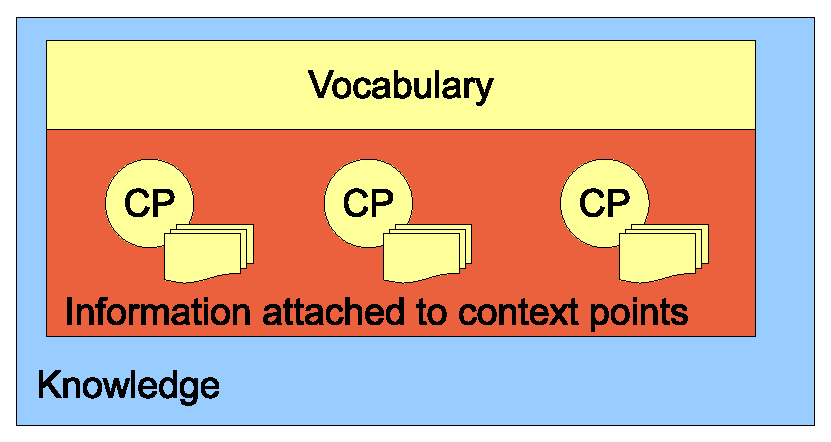
\includegraphics[width=0.40\textwidth]{knowledgecomponents.eps}
\caption{Knowledge components}
\label{fig:knowledgecomponents}
\end{figure}

Context points are means to store information with their coordinates, see previous chapter. Just exchanging sets of context points isn't sufficient in a semantic P2P system. Let's discuss it with an example we already know.

Alice stored information with coordinates: \\
(Shark, Alice, Alice, any, any, any, OUT).

Alice knows more, though. She knows that Shark {\it is a} P2P system. This fact isn't defined with coordinates. It is part of her vocabulary. Alice is willing to transmit information to others -- to Bob in our example. Apparently, it wouldn't be sufficient if she'd send just the context point. She should also send parts of her vocabulary which gives some background information.

In Shark, {\bf knowledge is set of context points with a vocabulary}. Knowledge is rarely created by developers. In most cases it is extracted from a knowledge base. Nevertheless, we want to demonstrate usage of knowledge with a little example.


\begin{verbatim}
SharkVocabulary v = new InMemoSharkKB();
Knowledge k = InMemoSharkKB.createInMemoKnowledge(v);
ContextPoint cp = null; // should not be empty
k.addContextPoint(cp);
SharkVocabulary kVocabulary = k.getVocabulary();
\end{verbatim}

We already know, that a vocabulary can be stored in a knowledge (line 1). There is an in-memory variant of knowledge which can be created with {\tt InMemoSharakKB} which isn't necessary that often in real applications. We use the vocabulary as parameter which becomes part of the knowledge.

We create a context point in line 3. It is empty which is not useful in real applications as well. We can add a context point to the knowledge. Line 4 illustrates the get-method for retrieving the vocabulary from an existing knowledge object.

Figure \ref{fig:knowledgecomponents} illustrates the parts of a knowledge object.


We can now summarise. Each {\tt SharkKB} contains a vocabulary, knowledge and has an owner, see figure \ref{fig:sharkkbcontent}.

\begin{figure}[t]
\centering
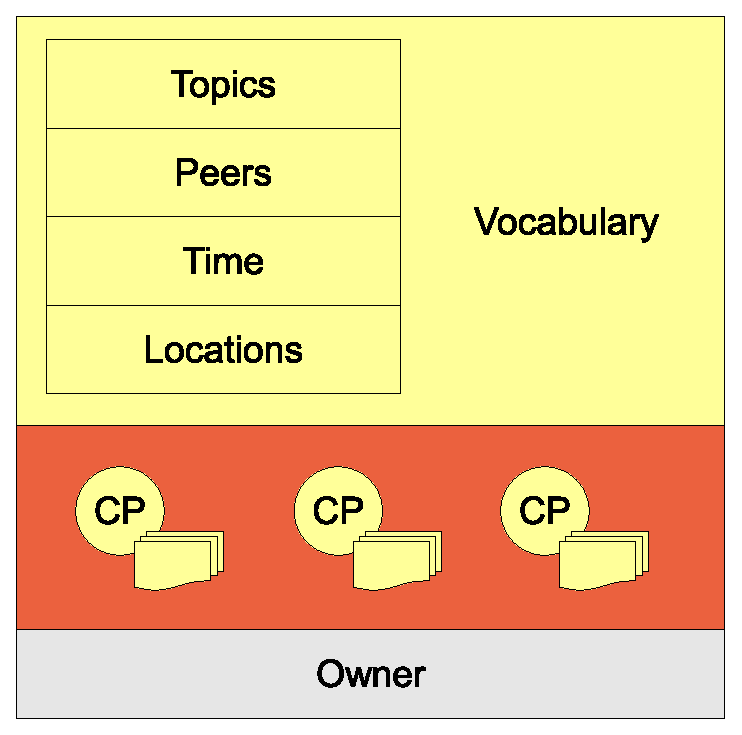
\includegraphics[width=0.50\textwidth]{sharkkbcontent.eps}
\caption{Parts of a Shark KB}
\label{fig:sharkkbcontent}
\end{figure}

\section{Knowledge Extraction}
\label{sec:extraction}
There are two quite complex operations provided by a knowledge base: Extraction and assimilation. We are going to explain both of them and start with extraction. Developers don't have do deal with these operation when using pre-defined knowledge ports. Nevertheless, the basic idea of extraction and assimilation should be understood.

Let's start with an example. (This and the following examples can be found on sharksystem.net under tutorials as {\tt ExtractionAssimilationExamples}.

\begin{verbatim}

this.kb = new InMemoSharkKB();

PeerSemanticTag alice =
  this.kb.createPeerSemanticTag("Alice",
       "http://www.sharksystem.net/alice.html",
       "mail://alice@wonderland.net");

// she owns that kb
this.kb.setOwner(alice);

// create background knowledge
Taxonomy tx = this.kb.getTopicsAsTaxonomy();

// describe programming languages and java as part of a taxonomy
TXSemanticTag pl = tx.createTXSemanticTag("PL",
   "http://en.wikipedia.org/wiki/Programming_language");

TXSemanticTag java = tx.createTXSemanticTag("Java",
   "http://en.wikipedia.org/wiki/Java_%28programming_language%29");

// move java "under" pl
java.move(pl);
// create two coordinates to fill that kb
ContextCoordinates ccPL = this.kb.createContextCoordinates(
   pl, alice, alice, // topic, originator, peer
   null, null, null, // remote peer, location, time
   SharkCS.DIRECTION_INOUT); / direction

ContextCoordinates ccJava = this.kb.createContextCoordinates(
   java, alice, alice,
   null, null, null,
   SharkCS.DIRECTION_INOUT);

ContextPoint cpPL = this.kb.createContextPoint(ccPL);
ContextPoint cpJava = this.kb.createContextPoint(ccJava);

cpPL.addInformation("something about programming languages");
cpJava.addInformation("something about java");

System.out.println("kb after initialisation: ");
System.out.println(L.kbSpace2String(this.kb));
\end{verbatim}

Each code example on the web page create a more or less lengthy output. We reduce the output to a minimum. This program prints out the newly created knowledge base.

\begin{verbatim}
owner: Alice

Vocabulary:
topics: PL->java
peers: Alice

Context Points
#0 (Java, Alice, Alice, any, any, any, inout)
#1 (PL, Alice, Alice, any, any, any, inout)
\end{verbatim}

\begin{figure}[t]
\centering
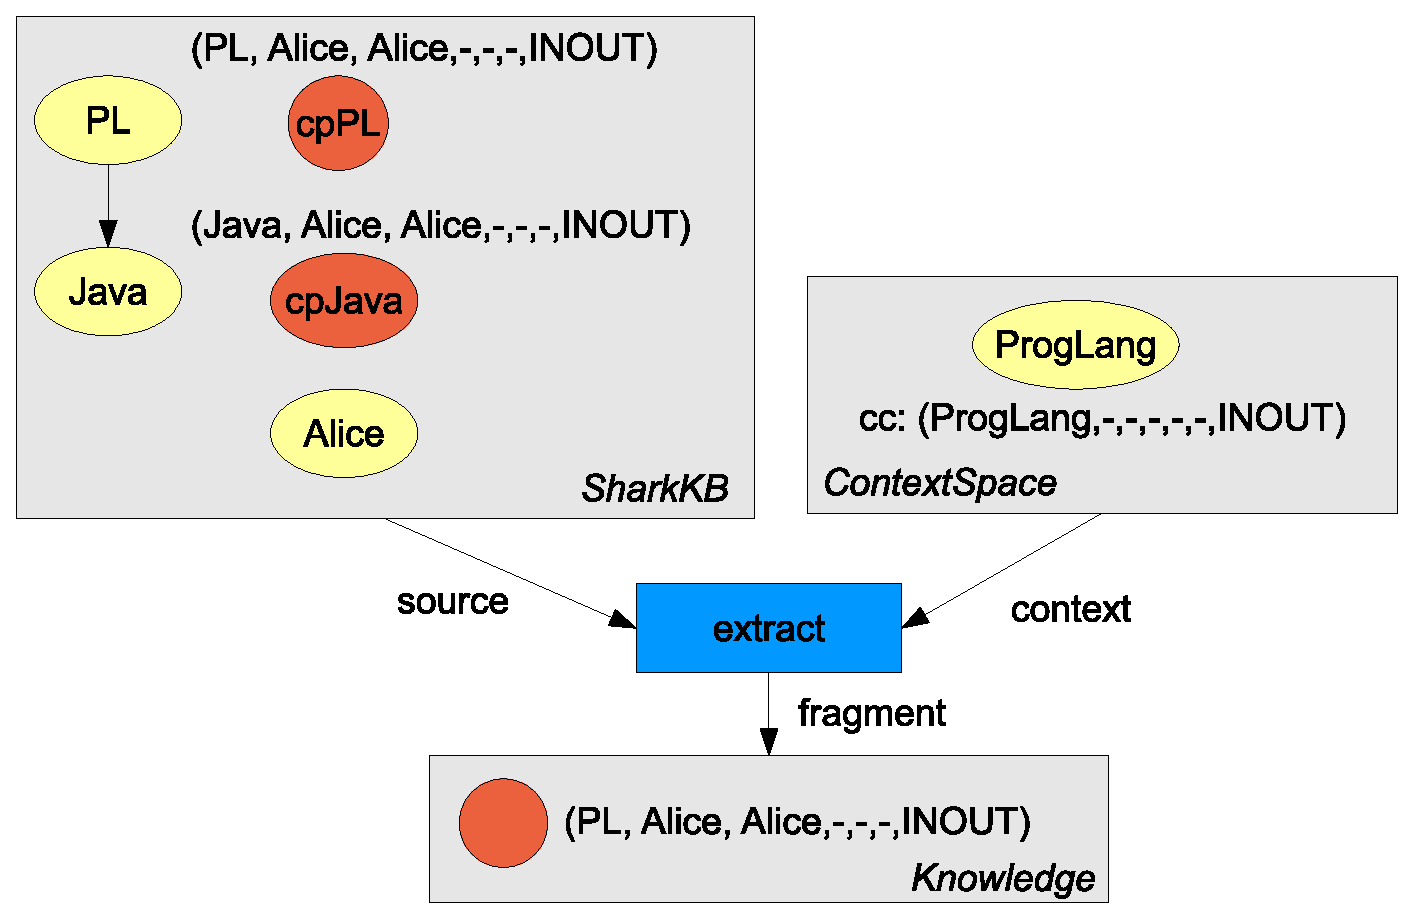
\includegraphics[width=0.60\textwidth]{extraction.eps}
\caption{Extraction example}
\label{fig:extraction}
\end{figure}

The code is not complicated:
An in memory knowledge base is created. Alice is described with a peer semantic tag. Java and programming languages are added to the {\it topic} set in that in our knowledge base. We also describe that Java {\it is a} programming language. Two coordinates are defined and information are added to both points. Both points have Alice as originator and peer. They differ in their topic dimension. One uses Java, the other takes - more general - programming languages as topic. Finally, we print out knowledge base content for debugging purposes.

Figure \ref{fig:extraction} illustrates most data structures: The {\tt SharkKB} with its three semantic tags and both context points are on the left upper side.
The tag labeled {\it ProgLang} is on the right side. It is not part of the knowledge base. It just exists in memory.

Let's continue our example with the following code.

\begin{verbatim}
SemanticTag plST =
   InMemoSharkKB.createInMemoSemanticTag("ProgLang",
      "http://en.wikipedia.org/wiki/Programming_language");

ContextCoordinates cc =
   InMemoSharkKB.createInMemoContextCoordinates(
      plST, null, null, null, null, null,
      SharkCS.DIRECTION_INOUT);

Knowledge k = SharkCSAlgebra.extract(kb, cc);

System.out.println(L.knowledge2String(k.contextPoints()));
\end{verbatim}

We create a single semantic tag describing programming languages.
We use a different name but the same subject identifier. Thus, this
tag {\it is identical} to the programming languages tag in our knowledge base.

We create a quite simple coordinate {\tt cc}. We just define the topic dimension. Any other dimension remains {\it any}. We use this coordinate as parameter for the {\tt extract} method. As a result, knowledge is returned with a single point as content and these coordinates:\\

{\tt PL, Alice, Alice, any, any, any, inout}\\

The coordinates are used as template, as query to the knowledge base. Extract looks for any context point that {\it fits} to that template. We use context coordinates in our first examples. {\it Interest} can be used as well. They are more flexible because they can contain more than one tag in each dimension.

Let's have a look on another example:

\begin{verbatim}
PeerSemanticTag aliceTag =
   InMemoSharkKB.createInMemoPeerSemanticTag(
      "A",
      "http://www.sharksystem.net/alice.html",
      null);

ContextCoordinates cc =
   InMemoSharkKB.createInMemoContextCoordinates(
      null,
      aliceTag,
      null, null, null, null, SharkCS.DIRECTION_INOUT);

Knowledge k = SharkCSAlgebra.extract(kb, cc);

System.out.println(L.knowledge2String(k.contextPoints()));

\end{verbatim}

A peer semantic tag is created in the first line. This tag can be seen as
template as well. We have described the subject identifier. Name and address are
more or less undefined. We use this tag as only relevant part to extract knowledge from our knowledge base.

The retrieved knowledge consists of two context point with these coordinates:\\

{\tt java, alice, alice, any, any, any, inout}\\

{\tt programming languages, alice, alice, any, any, any, inout}\\

Apparently, just a single context point in knowledge base fits to the given context. It is the point with topic {\it PL}.

It is time for a first summary. {\tt Extract} is a kind of query interface offered by the Shark knowledge base. The {\it source} must be a {\tt SharkKB}. It contains vocabulary and knowledge. {\it Context} is a kind of query. During extraction, any context point is added to the fragment that {\it fits} to the context. That {\it fitting} was very simple in this example. Context point coordinates must be {\it identical} to their counterparts in the context. Since any tags are identical to all other tags they can be used a joker sign.

There are variants of extraction.

\subsection{Extraction with fragmentation parameter}
Let's start with another example.

\begin{verbatim}
SemanticTag plST =
   InMemoSharkKB.createInMemoSemanticTag("PL",
      "http://en.wikipedia.org/wiki/Programming_language");

FragmentationParameter[] fps =
   new FragmentationParameter[SharkCS.MAXDIMENSIONS];

// set default - don't follow any direction
for(int d = 0; d < SharkCS.MAXDIMENSIONS; d++) {
   fps[d] = FragmentationParameter.getZeroFP();
}

// set topic dimension fragmentation
fps[SharkCS.DIM_TOPIC] =
   new FragmentationParameter(
      false, // don't follow super tags
      true, // follow sub tags
      1); //depth 1

ContextCoordinates cc =
   InMemoSharkKB.createInMemoContextCoordinates(
      plST, null, null, null, null, null,
      SharkCS.DIRECTION_INOUT);

Knowledge k = SharkCSAlgebra.extract(kb, cc, fps);

System.out.println(L.knowledge2String(k.contextPoints()));
\end{verbatim}

We have created our previous example. We create a semantic tag representing programming languages, create coordinates and extract information.
Result of this example both context points instead of a single point as in example one.

Fragmentation parameter make the difference. We have already learned about those parameter in the previous chapter. Tag {\it programming languages} has a single sub tag, namely {\it Java}. In this example, it is defined to follow sub tags but no super tags in topic dimension. No related tags are used in each other dimensions (defined by {\tt zeroFP}.

We use this array of parameters and use another variant of {\tt extract}.
\begin{figure}[t]
\centering
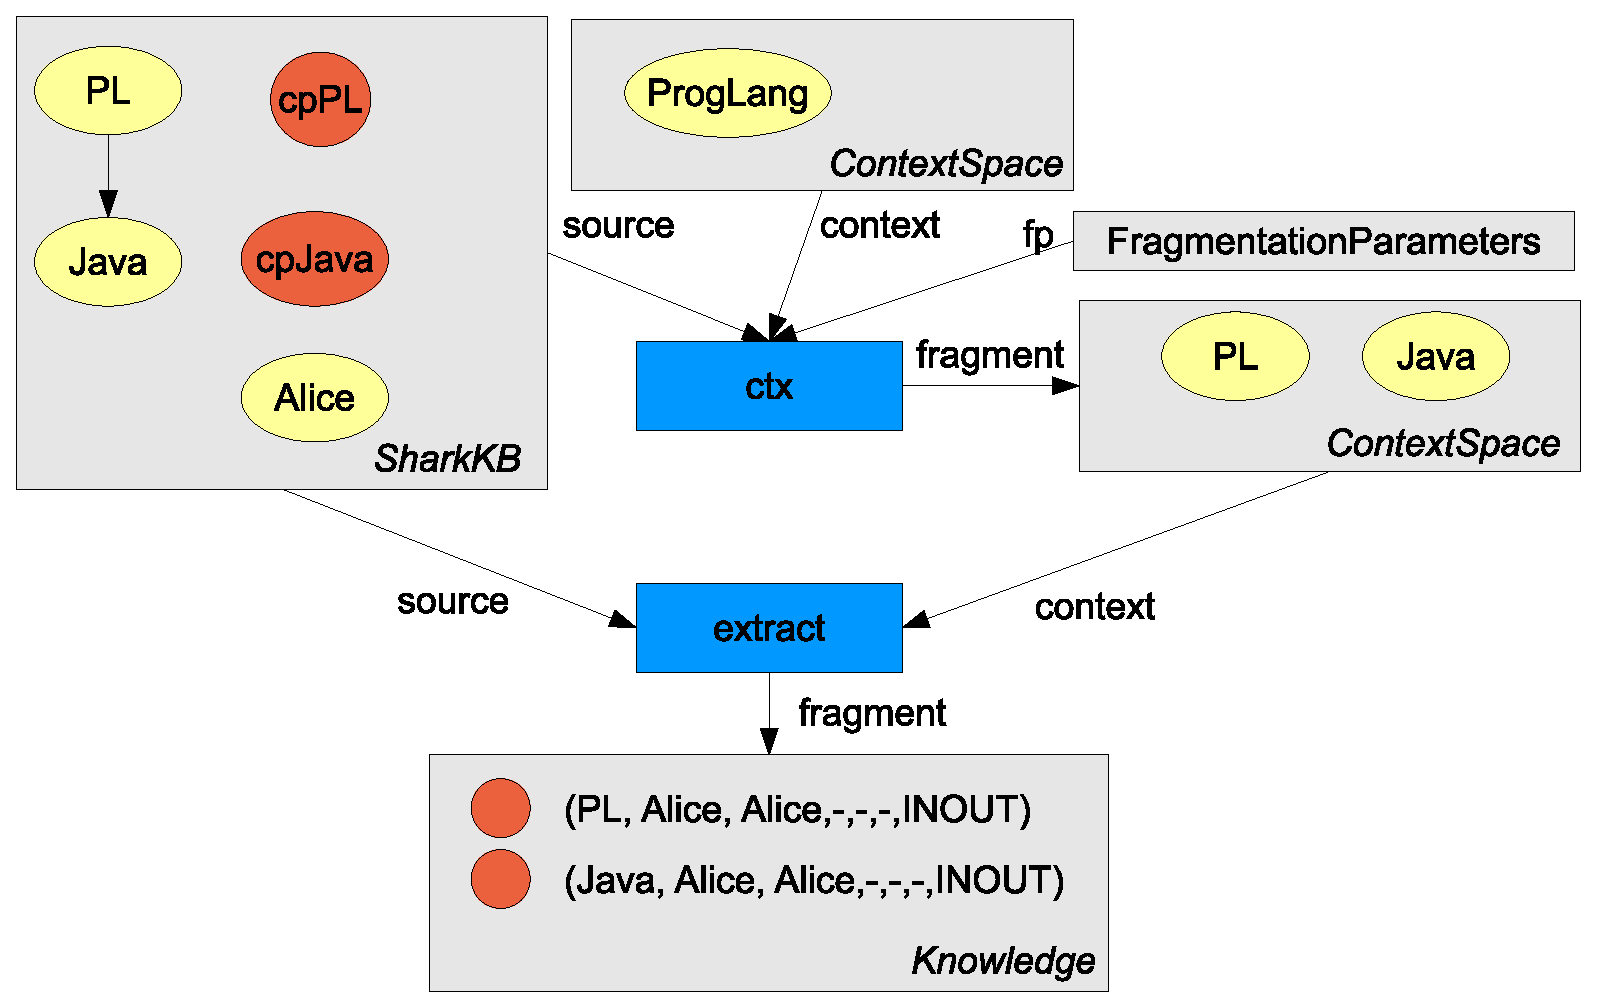
\includegraphics[width=0.60\textwidth]{extractionWithFPs.eps}
\caption{Extraction with fragmentation parameters}
\label{fig:extractionWithFPs}
\end{figure}

Figure \ref{fig:extractionWithFPs} illustrates the process.

\begin{enumerate}
\item A contextualization is made. The first parameter (our knowledge base in this case (and more specific: its vocabulary) is used as source. The second parameter ({\tt cc} in this case) is used as context. That {\tt ContextCoordinate} just contains one real semantic tag which describes programming languages. Fragmentation parameter configure contextualization process. The result is an {\tt SharkCS}. That context space contains two semantic tag on it topic dimension, see figure \ref{fig:extractionWithFPs}. Tag {\it PL} is {\it identical} to anchor {\it ProgLang}. Tag {\it Java} can be reached from {\it PL} under the constraints of fragmentation parameters.

\item The newly calculated context space is taken as context for the final extraction. Apparently, that context covers both context point in our knowledge base. Both are added the resulting knowledge fragment.
\end{enumerate}

This may sound complicated but the idea is simple. Remember our Bob in the early chapters. He is interested in programming languages in general but has no idea about Java. In Shark speech: Java is not part of his vocabulary yet. He can only ask for information of programming languages.

Alice knows about Java and the fact that Java {\it is a} programming language. This variant of {\tt extract} brings both together. Bob is able to describe his interest. Alice could receive that interest and expand it controlled by fragmentation parameter. Finally, she extracts knowledge.

This knowledge contains more than Bob has asked for. That is a major feature of the Shark framework. Bob can learn content (information) but also semantic tags and their relations.

We conclude this sub section with another example.
\begin{verbatim}

Taxonomy tTax = this.kb.getTopicsAsTaxonomy();
TXSemanticTag plTag =
   tTax.getSemanticTag(
      "http://en.wikipedia.org/wiki/Programming_language");

TXSemanticTag csharpST =
   tTax.createTXSemanticTag(
      "c#", "http://cshark.com");

csharpST.move(plTag);

ContextCoordinates ccCSharp =
   this.kb.createContextCoordinates(
      csharpST, null, null, null, null, null,
      SharkCS.DIRECTION_INOUT);

ContextPoint cp = this.kb.createContextPoint(ccCSharp);
cp.addInformation("information about c#");

SemanticTag javaST =
   InMemoSharkKB.createInMemoSemanticTag(
      "Java",
      "http://en.wikipedia.org/wiki/Java_%28programming_language%29");

FragmentationParameter[] backgroundFPs =
   new FragmentationParameter[SharkCS.MAXDIMENSIONS];

for(int d = 0; d < SharkCS.MAXDIMENSIONS; d++) {
   backgroundFPs[d] = FragmentationParameter.getZeroFP();
}

backgroundFPs[SharkCS.DIM_TOPIC] =
   new FragmentationParameter(true, true, 2);

ContextCoordinates cc =
   InMemoSharkKB.createInMemoContextCoordinates(
      javaST, null, null, null, null, null,
      SharkCS.DIRECTION_INOUT);

Knowledge k = SharkCSAlgebra.extract(kb, cc, backgroundFPs);
\end{verbatim}

We create another context point with topic {\it cSharp} which is sub tag of {\it programming languages}. We define fragmentation parameters that follows our topic taxonomy in both direction: up to super tags and down to sub tags. We use depth of 2. Extraction anchor is our {\it Java} topic. There are no other constraints. The result contains all three context points.

\subsection{Peer hierarchies}
We extend our program again.

\begin{verbatim}

PeerTaxonomy pTax = this.kb.getPeersAsTaxonomy();

TXSemanticTag alice =
   pTax.getSemanticTag(
      "http://www.sharksystem.net/alice.html");

PeerTXSemanticTag group =
   pTax.createPeerTXSemanticTag(
      "Group of Alice", "http://aGroup.org", (String)null);

alice.move(group);

ContextCoordinates groupCC =
   this.kb.createContextCoordinates(
      null, null, group, null, null, null,
      SharkCS.DIRECTION_INOUT);

ContextPoint cp = this.kb.createContextPoint(groupCC);

cp.addInformation("information from group");

FragmentationParameter[] backgroundFPs =
   new FragmentationParameter[SharkCS.MAXDIMENSIONS];

for(int d = 0; d < SharkCS.MAXDIMENSIONS; d++) {
   backgroundFPs[d] = FragmentationParameter.getZeroFP();
}

backgroundFPs[SharkCS.DIM_PEER] =
   new FragmentationParameter(false, true, 1);
//   new FragmentationParameter(false, false, 1);

Knowledge k = SharkCSAlgebra.extract(kb, groupCC, backgroundFPs);
}
\end{verbatim}

We have created a hierarchy as in our previous example but in the peer tag vocabulary.
Alice becomes part of a newly created {\tt group}. The following code is similar. Fragmentation parameter can be used in the same way. The combination
{\tt false, true} leads to knowledge that is filled with all context points. Try other true/false combinations and watch the results.

\subsection{Cutting peer hierarchies}
Lets review our last example. We have created a context point that has a group in its peer dimension. That's usual and advisable. It is convenient and efficient to create groups and add peers. Afterwords, we can add information and use those groups to define what peers (plural!) shall get these information.

Shark is a P2P system. Each peer can define its own group. Such a group can be compared with recipient list in e-mail. In a number of case, users don't want to reveal neither existence nor members of such a list, though.

This issue can be resolved with our final {\tt extract} variant. We continue our example.

\begin{verbatim}
PeerSemanticTag alice =
   this.kb.getPeerSTSet().
      getSemanticTag(
         "http://www.sharksystem.net/alice.html");

ContextCoordinates cc =
   this.kb.createContextCoordinates(
       null, null, alice, null, null, null,
       SharkCS.DIRECTION_INOUT);

FragmentationParameter[] backgroundFPs =
   new FragmentationParameter[SharkCS.MAXDIMENSIONS];

for(int d = 0; d < SharkCS.MAXDIMENSIONS; d++) {
   backgroundFPs[d] = FragmentationParameter.getZeroFP();
}

backgroundFPs[SharkCS.DIM_PEER] =
   new FragmentationParameter(true, true, 1);

Knowledge k = SharkCSAlgebra.extract(kb, cc, backgroundFPs, alice);
\end{verbatim}

This {\tt extract} variant works the same as the previous one at first. It uses fragmentation parameter to find fitting context points. This example will produce again knowledge with four pieces of information.

The extraction process does not end after context point extraction, though. Peer groups are post-processed: The fourth parameter ({\tt alice} in this case) is called {\it recipient}. Any group peer in context coordinates are removed by the recipient peer. All group peers are also removed from vocabulary. No group peer remains to which Alice belongs to.

We call this process {\it group cutting} and it is used to hide groups in general and member of groups to other peers in particular.

Take care: Groups are only cut if recipient is part of the group. A group cutting is not performed if each of the following cases is true.

\begin{itemize}
\item
There is a group in a peer dimension of a context point of the extracted knowledge.

\item
The receiving peer is not member of that group.
\end{itemize}

That situation can only occur when {\it any} tags are involved. Without {\it any} tags, a context point would only become part of the knowledge fragment if the context fits to its coordinates. {\it Fitting} means, it semantic tags are either identical or part of a group. Cutting will hide any group from remote peers automatically.

Problems may arise if unidentified peers are accepted as receiver. The remote peer is described with an {\it any} tag in that case. That tag fits to each peer but also to each peer group. Group cutting cannot be performed because identity of receiver is unknown. That special case can be handled when writing own knowledge port.

Using group hierarchies and {\it any} tags together can become a bit tricky. Take care!

\section{Knowledge Assimilation}
Whenever we talk about information and knowledge, we have to consider who created information and who shall be recipient.

Extraction is used to produce a bunch of information combined with a vocabulary to send both to another peer. Any peer is allowed to send knowledge to any peer under any circumstances.

A peer that receives knowledge has to consider several issues.

\begin{enumerate}
\item
Am I willing to receive any information from that peer?
\item
What topic am I'm interested in? More general, what general constraints do I have when receiving information?
\item
What dedicated information should I store?
\end{enumerate}

That process is called {\it assimilation}\footnote{Yes, the word is stolen from the Borg which play a quite relevant role in Star Trek.} in Shark. It starts when knowledge has been received. Peers are free in its reaction to incoming knowledge. In most cases, peers store information in which they are interested in. For such applications, the following section can be helpful.

Have a look at {\it example8} which can be found under {\it Knowledge Base Examples} on our web
site\footnote{http://www.sharksystem.net/codeExamples/sharkkb.zip}.

First lines in that example create a knowledge object that contains
two points:

\begin{verbatim}
(Java, Alice, Alice,-,-,-, inout)
(PL, Alice, Alice,-,-,-, inout)
\end{verbatim}

Let's see what happens afterwords in this example:

\begin{verbatim}
Knowledge k = ... // contains two cp now.
FragmentationParameter[] backgroundFPs = .. //zeroFP

//lets start with assimilation
STSet t = InMemoSharkKB.createInMemoSTSet();

// create java tag template
t.createSemanticTag(null,
   "http://en.wikipedia.org/wiki/Java_%28programming_language%29");

// create interest as filter for assimilation
Interest i = InMemoSharkKB.createInMemoInterest(
   t, null, null, null, null, null,
   SharkCS.DIRECTION_INOUT);

// create empty kb
SharkKB kb1 = new InMemoSharkKB();

// fill new kb with learning and no removing
SharkCSAlgebra.assimilate(kb1, i,
   backgroundFPs, k, true /*learn*/,
   false/* remove cp */);

System.out.println(L.kb2String(kb1));

\end{verbatim}

A semantic tag is created that has no name but an identity. Is represents {\it programming languages}. An interest is created that contains just that tag.

An empty knowledge base ({\tt kb1}) is created. Afterwords, the assimilation is started and uses the empty knowledge base as target and the knowledge as source.
{\tt backgroundFP} is a zero parameter set - depth is zero in each dimension.

\begin{figure}[t]
\centering
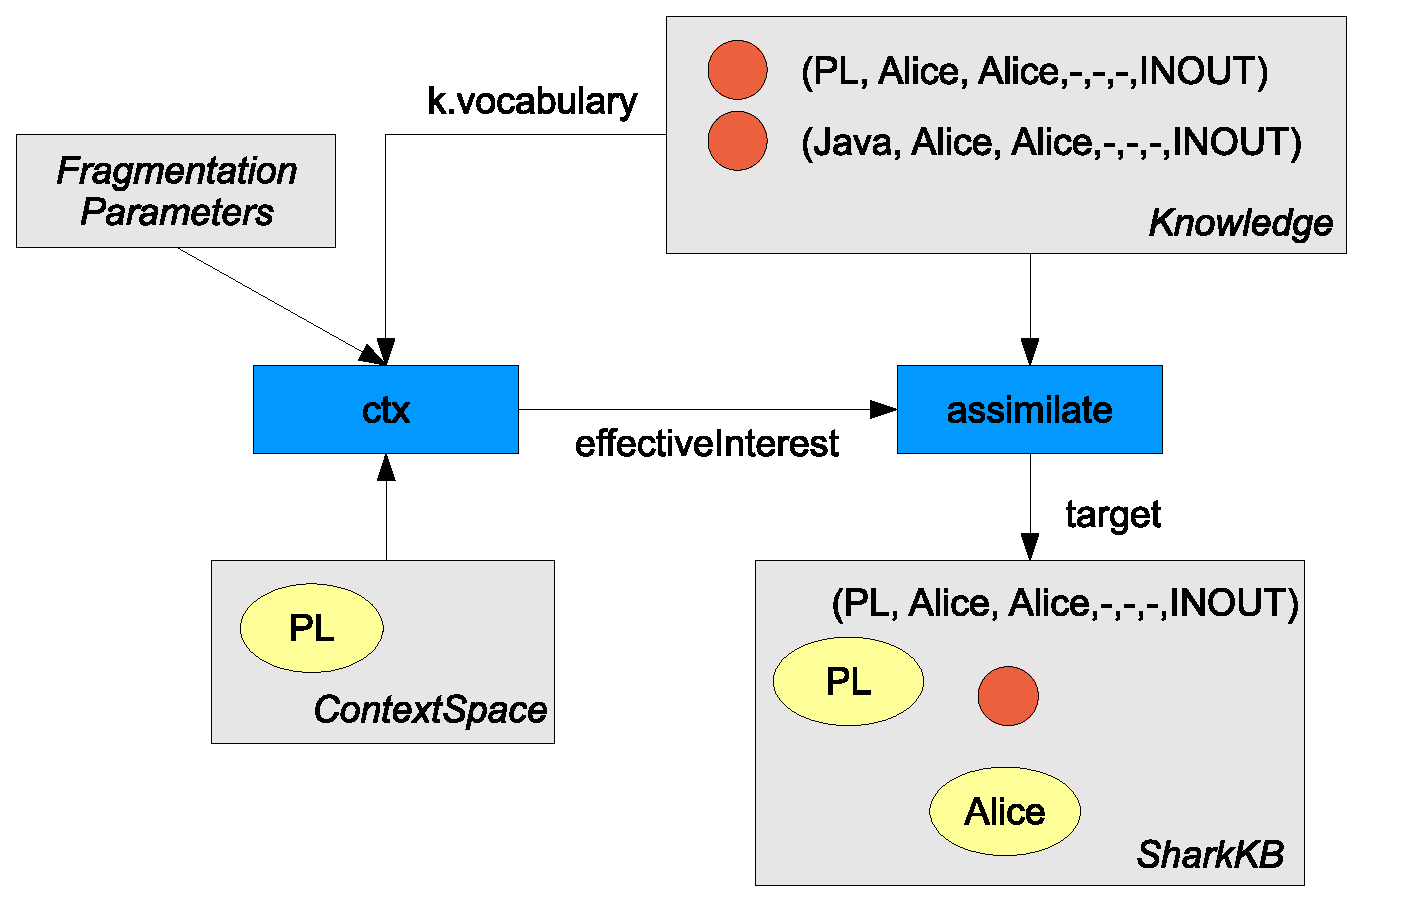
\includegraphics[width=0.70\textwidth]{assimilation.eps}
\caption{Assimilation}
\label{fig:assimilation}
\end{figure}

Figure \ref{fig:assimilation} illustrates the process. It consists on two general steps.

\begin{enumerate}
\item
A contextualization is performed, see left side in figure \ref{fig:assimilation}. Knowledge vocabulary is taken is source. The interest serves as context and the fragmentation parameter are the third parameter. The result is called {\it effective interest}. What is that good for?

Vocabulary of sender and receiver might differ. Thus, there can be tags in knowledge which are unknown to recipient. The receiving peer has a chance to learn tags in this step. It defines anchor and fragmentation parameter.

Receiver isn't interested in our example code. Fragmentation parameter are {\it zero parameter} in each dimension. In that case, contextualization is simple: Each tag that is in receiver's interest and the knowledge vocabulary is also part of the {\it effective interest}.

\item
As we could see, an interest spans a context space. So does the {\it effective interest}. It covers a space which is of interest of receiving peer. Now, each context point in knowledge is added to the target knowledge base which is in this space. All other context points are ignored.
\end{enumerate}

Content of kb1 after assimilation is this:

\begin{verbatim}
Vocabulary:
topics: Java
peers: Alice
Content:
#0: (PL, Alice, Alice, any, any, any, inout)
\end{verbatim}

Seems to be pretty obvious. We have learned about Java and Alice and both words are added to our vocabulary\footnote{and brought us closer to perfection. I couldn't hesitate to frame with phrases from the Borg queen.}. Two context points are added as well.

Have a closer look at the assimilated context point. Alice is in the {\it remote peer} dimension and not any longer in the {\it peer} dimension.

It is assumed that knowledge from another peer is assimilated. Thus, we have to change perspective. The remote peer would pronounce itself as peer. The recipient would recognize it as {\it remote} peer, though. Moreover, a peer can declare information to be sent. Now, those information are received. We cannot assume that the peer will also think that those information have to be transmitted immediately. Assimilation makes some changes in dimensions:

\begin{itemize}
\item Peer and remote peer dimension change places.
\item Direction is changed. OUT and INPUT becomes IN. NOTHING remains unchanged. Direction IN wouldn't be accepted anyway because it wouldn't match to an receiving interest.
\end{itemize}

There are two parameter left to be explained. Let's start with the easy one:
{\tt deleteAssimilated} is a boolean value. Set to {\tt true} each context point that was assimilated is removed from knowledge. Applications which use a single knowledge base should always use the {\tt true} setting. That avoids re-assimilation of same knowledge by different knowledge ports. It makes no sense to add knowledge twice. Once added to the local knowledge base it can be removed. Following knowledge port has less to do. Applications with more than one knowledge base will have probably another strategy.

They {\tt learnTags} parameter is a boolean value. A peer learns vocabulary from received knowledge if set {\tt true}. The local vocabulary will remain unchanged otherwise. How could a peer learn vocabulary?

Review our last example. Knowledge arrived with two context points. One is about {\it Java}, the other about {\it programming languages}. The effective interest contained only {\it programming languages} due to the zero fragmentation parameter.

Lets assume, we have had chosen a more broader parameter set. Maybe we have allowed to extract related tags to {\it programming languages}. In this case, {\it Java} would have become part of effective interest and second context point would have been added to the local knowledge base. If {\tt learnTags} would be set to true, {\tt kb1} would contain two points then:

\begin{verbatim}
(Java, Alice, Alice,-,-,-, inout)
(PL, Alice, Alice,-,-,-, inout)
\end{verbatim}

Receiver would have learned tag {\it Java} and two context points are added.

Just a single context point would exists after assimilation if {\tt learnTags} would have set to {\tt false}:

\begin{verbatim}
(PL, Alice, Alice,-,-,-, inout)
\end{verbatim}

No {\it Java} tag would have be learned. But note, the second context was assimilated as well! We haven't changed anything on fragmentation parameter. What happened?

Assimilation algorithm decides whether a context point gets added to the local knowledge base or not. That decision is made independently if tags are to be learned or not. There can be context points which have tags in their dimensions which are unknown in the local vocabulary. Such tags are replaced by the closest locally known tags.

In our example, the receiving peer refused to learn the tag {\it Java}. The closest tag to {\it Java} is {\it programming languages}. Thus, all information are added to the context point as well.

When running the program, you'll see that {\tt (PL, Alice, Alice,-,-,-, inout)}
has two attached information.

That's it. We won't discuss any method from {\tt SharkKB}. Most of them are pretty obvious. We strongly recommend to make the exercises. They help to understand the concept. And they are not that difficult. Solutions can be found on the sharksystem.net web page. But it's better making them alone. Good luck!

\section{Exercises}

\chapter{Knowledge Ports}
\label{sec:knowledgePorts}
We have learned a lot about vocabulary and knowledge. Now, we can discuss communication. {\it Entities} communicate in each distributed system. Client-Server systems define two classes of {\it entities}. Clients communicate with servers. Each entity has its designated role in each communication act. They can change roles, though. A computer that is server in one communication can be client in another one.

Shark based applications are P2P applications. Each Shark peer should be aware of receiving messages. Each Shark peer can send anytime any other peer a message. Shark communication paradigm can be compared with a crowded party. People who might never seen before exchange some words and go away. Maybe they see again, maybe not. People can say something. Maybe it is understood or not.
People can also exchange phone numbers and addresses. After that, they can talk even if they are no longer at this party. 

That's the very idea of Shark. Peers can communicate whenever they want to but they have no obligation to answer in a defined manner. Shark makes no constraints about communication behavior. It's up to the application.

A leaflet application might deliver an advertisement to any peer. Certainly, it won't be seen as {\it rude} if peers don't react. A leaflet sender can not assume a {\it thank you} or whatever.

Another application might be a decentralized social network\footnote{SharkNet is
a growing example. It actually is a social network based on Shark, see our web page for project status.}. In such application it can be helpful to know if information has received its destination or not. Such handshakes can be coded by applications programs. We'll see an example in section \ref{sec:chatkp}.

Communication requires a protocol. This protocol is called {\it Knowledge Exchange Protocol (KEP)}. It has just two commands: 

\begin{description}
    \item[Expose] sends an interest to a peer.
    \item[Insert] sends knowledge to a peer.
\end{description}

Application logic can be implemented with {\it Knowledge Ports} in Shark which are sometime called {\it Sharklets}. It is a quite slim interfaces. 

Creating your own application specific knowledge port is simple as to be seen in the following code:

\begin{verbatim}
public class MyKP extends KnowledgePort {
   public MyKP(SharkEngine se) {
      super(se);
   }

   @Override
   protected void doInsert(Knowledge knowledge, 
                           KEPConnection kepConnection) {

      // do something useful here - or not
   }

   @Override
   protected void doExpose(SharkCS interest, 
                           KEPConnection kepConnection) {

      // do something useful here - or not
   }
}
\end{verbatim}

We will discuss the KEP protocol itself very briefly in this chapter. Shark creates messages which are sent over the network.

This chapter discusses how to write your own knowledge port. Shark has some predefined knowledge port. They will be presented. The most important is our {\tt StandardKP}. We claim, that most applications can be implemented with it by setting appropriate parameters. 

\section{Implementing your own Knowledge Port}
Each knowledge port must be derived from {\tt KnowledgePort}. Each knowledge port must run with a {\tt SharkEngine}, see next chapter. Thus, each knowledge port {\it must} call the constructor that sets this engine.

\begin{verbatim}
public class MyKP extends KnowledgePort {
   public MyKP(SharkEngine se) {
      super(se);
   }

//...
\end{verbatim}

{\tt KnowledgePort} is abstract because two methods are abstract which have to be implemented by non-abstract knowledge ports.


\begin{verbatim}
   @Override
   protected void doInsert(Knowledge knowledge, 
                           KEPConnection kepConnection) {
      // do something useful here - or not
   }

   @Override
   protected void doExpose(SharkCS interest, 
                           KEPConnection kepConnection) {
      // do something useful here - or not
   }
}
\end{verbatim}

Abstract class {\tt KnowledgePort} offers a number of useful methods which are explained throughout that section and can also be found in the online API description\footnote{http://sharkfw.sourceforge.net/api/current/net/sharkfw/peer/KnowledgePort.html}.

\subsection{KEPConnection}
Knowledge ports are called when KEP message reaches a peer. They have to handle either interests or knowledge. Any knowledge ports must implement two methods for that reason: {\tt doExpose} to handle interests and {\tt doInsert} to handle knowledge. 

Both methods have two parameters: First is an interest or knowledge. Second is a {\tt KEPConnection} object. We are going to explain some details of that object in this section.

{\tt KEPConnection} allows to check whether an message was encrypted and / or signed.

\begin{verbatim}
protected void doExpose(SharkCS interest, 
                  KEPConnection kepConnection) {
//...
  if( kepConnection.receivedMessageEncrypted() {
    // message was encrypted
  }
  if(kepConnection.receivedMessageSigned()) {
    // message was signed
  }
}
\end{verbatim}

\subsubsection{Reply}
Peer often want to reply to incoming interests or knowledge. A reply can be an arbitrary number of expose and insert messages. In other words, a peer can reply with interests and knowledge. 

A reply is send by means of the {\tt KEPConnection} object by calling {\tt expose} or {\tt insert} with appropriate parameters.

There are a three variants of {\tt expose}. Have a look at the following code fragment.

\begin{verbatim}
Interest i = // create an interest
try {
 kepConnection.expose(i);
} catch (SharkException ex) {
 // do something 
}
}
\end{verbatim}

The actual interest is less important for this example. We just need one. Now, {\tt kepConnection} is used to send this interest to the peer from whom we have received the KEP message in the first place. In short: It is a direct reply. An exception can be thrown if something went wrong during delivery.

There is another variant:

\begin{verbatim}
String address = "mail://alice@wonderland.gov";
try {
   kepConnection.expose(interest, address);
} catch (SharkException ex) {
   // do something
}
\end{verbatim}

The reply is sent to a dedicated address instead to the sending peer. The final variant takes an array of addresses instead a single address, see online documentation. The interest is sent to each address in the list.

The same concept is used if knowledge is to be sent as reply. Note, there is no method that sends knowledge just to the sending peer. It is for developers safety and not for their punishment.

We figured that developers tend to become confused by all those peers which can be seen as sender. Shark philosophy is that interests tend to be commonly available but knowledge not. We think, that sending knowledge must happen deliberately. Let's have a look of different kind of sender.

\subsection{Physical and logical sender}
\label{sec:knowledgePorts:sender}

\begin{figure}[t]
\centering
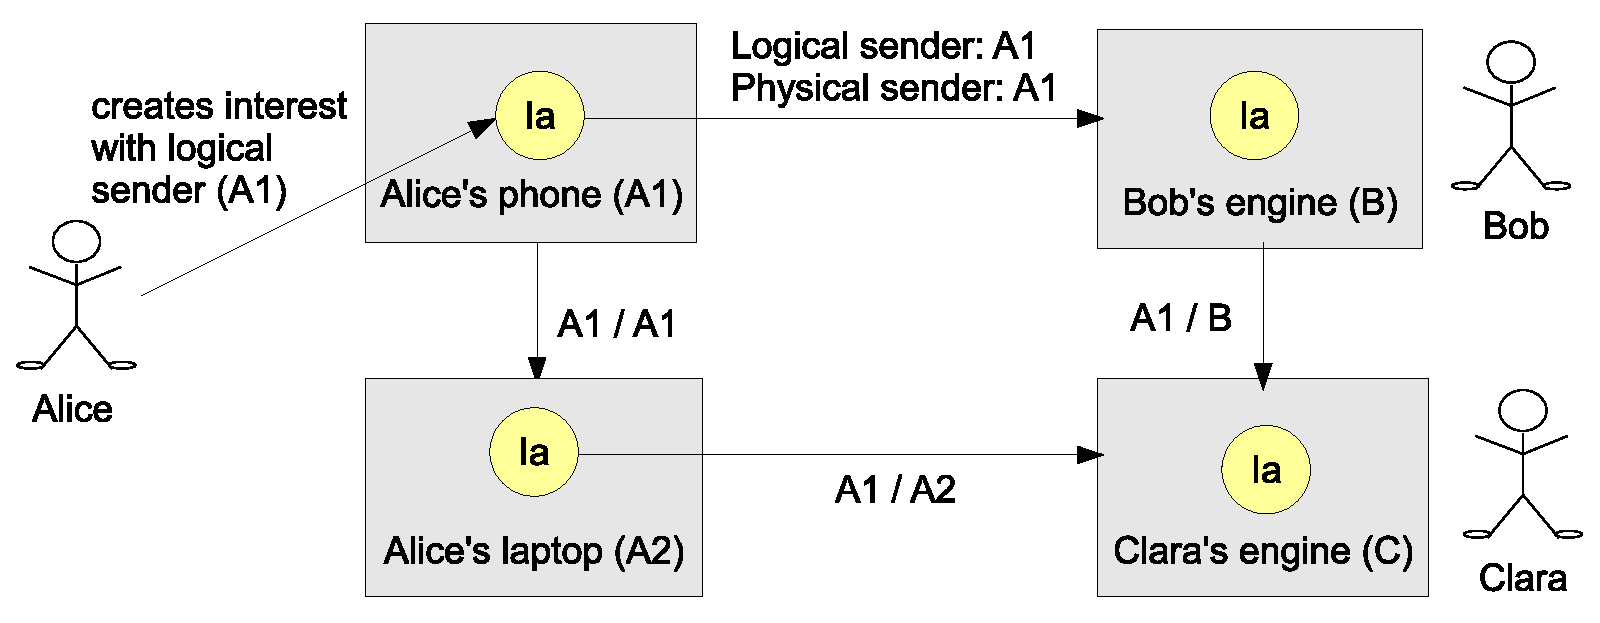
\includegraphics[width=0.80\textwidth]{physicalAndLogicalSender.eps}
\caption{Physical and logical sender}
\label{fig:physicalAndLogicalSender}
\end{figure}

Whenever a peer has received a KEP message there was a {\it physical sender} which is a computer, smartphone, etc. that issued the message. That message can be encrypted and signed. Neither of them ensures that the physical sender is actually the peer that is described in {\it peer dimension} of the interest or knowledge. That peer is called {\it logical sender}. When we talk about a {\it sender}, we already mean the {\it logical sender}.

A {\it logical sender} can create a message, can even sign and encrypt but can store it in another device which transmits this message to others. Thus, the other devices or peers can act as proxies or relays. Recipients can decide whether to reply to the proxy or directly to the {\it logical sender}. 

Figure \ref{fig:physicalAndLogicalSender} illustrates the relation between {\it logical} and {\it physical} sender. Alice creates an interest in this example. She stores that interest on her device A1. She also decided to choose A1 as logical sender. Note, each peer, each user is free to define a logical sender address. We have already defined an number of addresses for peers throughout that book. All addresses in peer semantic tags are {\it logical} addresses and can freely be chosen by users.

In this example, Alice choses A1 as logical address and stores her interest also on A1. She meets Bob and exposes her interest. In that case, physical and logical sender are identical.

Bob can forward Alice's interest (unchanged) to Clara. Alice is still logical sender but Bob's device is logical sender. 

Alice could also synchronize her data to another device, e.g. her laptop. Her interest could also be sent from her laptop to Clara. In that case, A1 is still logical but A2 is physical sender.

{\tt KEPConnection} offers several methods to reply to incoming interests. The more convenient methods reply to the {\it physical} sender. In most cases, this would be an appropriate choice but not in any. 

Moreover, information of physical sender are not stored in interests or knowledge. That information is only available when receiving that data.
Applications who need physical sender information are required to save it.
Physical sender address can be retrieve from the connection object.

\begin{verbatim}
PeerSemanticTag sender = kepConnection.getSender();
String[] addresses = sender.getAddresses();
\end{verbatim}

We encourage to defines recipient addresses explicitly. That makes your code more transparent for other programmers.

Shark allows signing and encrypting. Shark only offers End-to-End-Encryption. Physical sender don't play any role in those scenarios. Logical sender sign and encrypt. Physical devices are only means for transportation.

\subsection{Sending initial messages}
It isn't enough to wait for incoming requests. One peer must start talking.

{\tt KnowledgePort} objects support methods for sending interests and knowledge. The following code is a scetch of its usage.

\begin{verbatim}
Knowledge k = ...
Interest i = ...
PeerSemanticTag peer = ...
this.sendKnowledge(k, peer);
this.sendInterest(i, peer);
\end{verbatim}

The code is straightforward. We need a peer and either knowledge or an interest which can be delivered. Sending might fail either for security reasons or network problems. Exception are thrown in either case.

A KEP message is send in case of success and be be handled by the receiver, more specific by a receivers {\tt KnowledgePort} objects. Note, message can send with each running knowledge port. The sending port has no privileges over others. A reply on a sent message is handled as any other message and offered to each active knowledge port.

Thus, sending a message requires at least a single active knowledge port. 
There are no methods (yet) that allows developers to send {\it interest} or {\it knowledge} without a {\tt KnowledgePort} object. In the rare case of a peer that has no knowledge a workaround is proposed: Implement your own knowledge port and leave {\tt doExpose} and {\tt doInsert} empty. Now you have a knowledge port that actually has no effect on incoming messages but can be used to send messages.

\subsection{Creating a knowledge port}
Now we are ready to instantiate a knowledge port. We need a {\tt SharkEngine} first, see chapter \ref{sec:sharkengine} for details. Afterwards, we can bring our knowledge port into existence and action:

\begin{verbatim}
SharkEngine se = new J2SEAndroidSharkEngine();
KnowledgePort kp = new MyKP(se);
\end{verbatim}

The port is up and running now. Knowledge port management is discussed in the {\tt SharkEngine} chapter.

\subsection{KP Listener}
{\tt KnowledgePort} objects can be observed. The following code implements a class that listens to knowledge port activities.

\begin{verbatim}
public class MyKPListener implements KPListener {
  public void exposeSent(KnowledgePort kp, 
                         SharkCS sentMutualInterest) {
    System.out.println("expose received");
  }

  public void insertSent(KnowledgePort kp, 
                         Knowledge sentKnowledge) {
    System.out.println("insert received");
  }

  public void knowledgeAssimilated(KnowledgePort kp, 
                                   ContextPoint newCP) {
    System.out.println("KP has assimilated something");
  }
}
\end{verbatim}

This class implements the {\tt KPListener} interface that comprises three methods which are implemented in a quite naive way.

A listener must be added to a knowledge port. Let's extend our example code from previous section:

\begin{verbatim}
SharkEngine se = new J2SEAndroidSharkEngine();
KnowledgePort kp = new MyKP(se);
KPListener myListener = new MyKPListener();
kp.addListener(myListener);
\end{verbatim}

{\bf Knowledge port developer have to trigger those listener events!} The {\tt KnowledgePort} class just offers methods to subscribe and remove listeners.
It does {\it not} trigger e.g. a {\tt exposeSent} event. This is up to knowledge port developers!

Triggering those events is very simple, though. The following code can be  called inside any knowledge port object.

\begin{verbatim}
// get or create interest and send it
Interest i = ...
// notify listeners that an interest was exposed
this.notifyExposeSent(this, i);

// create or get knowledge and send it
Knowledge k = ...
// notify listener about send knowledge
this.notifyInsertSent(KnowledgePort kp, k);

// get context point and write to knowledge base
ContextPoint cp = ...
// notify listeners
notifyKnowledgeAssimilated(KnowledgePort kp, cp);
\end{verbatim}

\subsection{Other methods}
Knowledge ports can be stopped and restarted again.

\begin{verbatim}
..
KnowledgePort kp = ...
kp.stop();
..
kp.start();

boolean started = kp.isStarted();
\end{verbatim}

A stopped knowledge port does not get any KEP message until it is restarted again. 

Each knowledge port can hold a knowledge base. We have added this feature into the most abstract superclass because most knowledge ports will need a knowledge base for operations.

\begin{verbatim}
..
SharkKB kb = ...
kp.setKB(kb);
..
kb = kp.getKB();
\end{verbatim}

Most knowledge ports will work with an interest. There are methods to set and get interests.

\begin{verbatim}
..
Interest i = ...
kp.setInterest(i);
..

i = kp.getInterest();

// does kp have a receiving  and/or sending interest?
boolean receivingInterest = kp.isIKP();
boolean sendingInterest = kp.isOKP();
\end{verbatim}

Let's summarize. Knowledge ports are {\it the element} that stores the actual application logic of peers. Knowledge ports work independently from each other. Thus, a peer can instantiate a number of ports that perform different tasks.

Writing a knowledge port is as difficult or as easy as writing a Servlet. 

Moreover, there are some knowledge port implementation already in the framework. We guess that this number of predefined knowledge ports will increase over the years and releases. Next section will explain the most important knowledge ports. We start with the most generic port which is called {\tt StandardKP}. It can be configured in different ways. We hope that this generic port can solve most applications needs just be configuration. Reading and understanding the following section can seriously reduce your development time. Enjoy!

\section{Exercises}

\begin{enumerate}
\item 
Create a knowledge port that... Implement your own KP.
\end{enumerate}

\chapter{Predefined Knowledge Ports}
Knowledge ports are building blocks of Shark based applications.
Each Shark project will create its own knowledge port. Some are
already shipped with the framework. Number of such ready-to-use
ports will increase which each new version. The first and most flexible
implementation is the {\tt StandardKP} though.

\section{StandardKP}
\label{sec:knowledgePorts:StandardKP}
The  {\it Shark basic scenario} was explained in section \ref{sec:concepts:baseScenario}: Alice and Bob met. Both are interested in {\it P2P system}. Both found out their mutual interest by means of interest exchange. Finally, knowledge was transfered.

{\tt StandardKP} was developed to serve such scenarios. This section reveals how this basic scenario can be implemented with a few lines of code.

But let's start from the beginning: {\tt StandardKP} extends {\tt KnowledgePort}. It isn't abstract and implements {\tt doExpose()} and {\tt doInsert()} it triggers {\tt KPListener} objects.

Each {\tt StandardKP} must be instantiated with an interest and a knowledge base. This KP can actually be seen as the guard that serves as an extractor and
assimilator of knowledge. The interest can be seen as a filter for both exporting and importing.

We are going to finish the introduction and start with the program. Actually, we are going two write two programs: One plays the role of Alice, the other the role of Bob. Source code can also be found on sharksystem.net under tutorials.

The following section will contain the whole Alice program, next one will contain Bob. Relevant algorithms are explained afterwords.

\subsection{Alice and Bob basic scenario}
\subsubsection{Alice}
\begin{verbatim}
public class Alice implements KPListener {
  public static SharkEngine aliceSE;

  public static void main(String[] args) throws ... {
    // Create a new SharkEngine
    aliceSE = new J2SEAndroidSharkEngine();

    // Create a new knowledge base for this Alice
    SharkKB kb = new InMemoSharkKB();

    // Create a peer to describe the topic "Shark"
    SemanticTag shark = kb.createSemanticTag
                           ("Shark",
                            "http://www.sharksystem.net/");

    // Create a peer semantic tag describing Alice herself
    String[] aliceAddr = new String[1];
    aliceAddr[0] = "tcp://localhost:7070";

    PeerSemanticTag alice = aliceKB.createPeerSemanticTag(
                              "Alice",
                              "http://www.sharksystem.net/alice.html",
                              aliceAddr);

    // Alice owns this SharkKB
    aliceKB.setOwner(alice);

    // Create new coordinates before creating a ContextPoint
    ContextCoordinates cc = aliceKB.createContextCoordinates(
                              sharkST, /* topic */
                              alice, /* originator */
                              alice, /* peer */
                              null, /* remote peer: any*/
                              null,  /* time: any */
                              null, /* place: any */
                              SharkCS.DIRECTION_OUT);

    // Create a ContextPoint to add information to
    ContextPoint cp = aliceKB.createContextPoint(cc);

    // Add a string to the ContextPoint at the given coordinates
    cp.addInformation("I like Shark");

    // Create a StandardKP with engine, kb and interest
    StandardKP kp = new StandardKP(aliceSE, cc, aliceKB);

    // set up listener
    Alice alicePeer = new Alice();
    kp.addListener(alicePeer);

    // Start listening at TCP port 7070
    aliceSE.startTCP(7070);

    // Now the peer is passively waiting for incoming traffic

    // Create description if Bob
    PeerSemanticTag bob = aliceKB.createPeerSemanticTag(
                            "Bob",
                            "http://www.sharksystem.net/bob.html",
                            "tcp://localhost:7071");

    // publish interest to start communication
    // assumes that bobPeer is already up and running
    aliceSE.publishKP(kp, bob);
  } // end main methods

  /* KPListener implementation */
  public void exposeSent(KnowledgePort kp,
                         SharkCS sentMutualInterest) {
    // ignore
  }

  public void insertSent(KnowledgePort kp,
                         Knowledge sentKnowledge) {
    // Alice shuts down after sending knowledge
    System.out.println(
       "Alice has sent something - enough for today...");
    aliceSE.stop();
  }

  public void knowledgeAssimilated(KnowledgePort kp,
                                   ContextPoint newCP) {
    // ignore
  }
} //end Alice class
\end{verbatim}

Only fourteen lines of code are required to write a P2P program that does an useful job. Additional line are required to implement the {\tt KPListener}. We had some larger programs when we explained knowledge extraction etc. That is because {\tt StandardKP} perfoms the whole communication between knowledge base and external peer(s).

Let's investigate the program. Most of it was explained in previous chapter. We create a {\tt SharkEngine} which makes up the peer. We have created a {\tt SharkKB} which holds semantic tags and information.

A semantic tag is created that describes {\it Shark}. A peer semantic tag is created describing Alice herself. In this example, she has just a single address: A TCP port at local host. That's not advisable for real applications but it's a good decision testing.

{\tt ContextCoordindates} are created. They use {\it Alice} as originator and peer and {\it Shark} as topic. Information shall be sent which is defined by
{\tt DIRECTION\_OUT}. A context point is created and a brief information added.

Neither of those lines are new. New is creation of the {\tt StandardKP} with three parameters: the {\tt SharkEngine}, the {\tt interest} (we re-use our coordinates) and the {\tt SharkKB}. That's it. Out {\tt StandardKP} has anything it needs: It knows what is Alice willing to talk about and it knows where to store and/or retrieve information.

A KPListener is set up afterwords - just to illustrate it's usage.

\begin{verbatim}
aliceSE.startTCP(7070);
\end{verbatim}

This line tells the engine to open a TCP port and to accept incoming KEP messages. Now the Alice peer is ready to retrieve information.

In this example, Alice initiates communication. A peer semantic tag is used to describe bob. His peer is listening at port 7071 on the same machine which will hardly be used in real applications but in tests.

\begin{verbatim}
aliceSE.publishKP(kp, bob);
\end{verbatim}

This line forces the engine to take the {\it interest} from the {\tt kp} and send it to {\tt bob}. An {\it expose} message is sent from Alice to Bob. That's it. Communication has started.

The KPListener implementation is trivial. Alice peer stops communicating after sending a single knowledge object, see {\tt insertSent} implementation.

\subsubsection{Bob}
The following program implements Bob who is also interested in Shark. He wants just receive information but not send anything. The following lines are just the main method of the Bob peer.

\begin{verbatim}
// SharkEngine bobSE is declared as member variable
// create engine
bobSE = new J2SEAndroidSharkEngine();

// Create an in memory knowledgebase for information storage
SharkKB kb = new InMemoSharkKB();

// Describe Shark
SemanticTag shark = kb.createSemanticTag("SharkFW",
                      "http://www.sharksystem.net/");

// Create a peer to describe ourselves (Bob)
String[] bobAddr = new String[1];
bobAddr[0] = "tcp://localhost:7071";

PeerSemanticTag bob = kb.createPeerSemanticTag("Bob",
                        "http://www.sharksystem.net/bob.html",
                        "tcp://localhost:7071");

// Create an interest
ContextCoordinates interest = kb.createContextCoordinates(
    shark, /* topic */
    null, /* originator: any */
    bob, /* peer */,
    null, /* remote peer: any */
    null, /* time: any */
    null, /* location: any */
    SharkCS.DIRECTION_IN /* looking for information */
);

// Create Standard knowledge port
StandardKP kp = new StandardKP(bobSE, interest, kb);

// Start listening at TCP port 7071
bobSE.startTCP(7071);
\end{verbatim}

\subsection{doExpose}
Both program are quite short. That's because the application logic is hidden in the {\tt StandardKP}. We are going to describe the algorithm that is performed when an interest is received.

Figure \ref{fig:StandardKP_expose} summarizes the standard expose process.
Yes, that figure is confusing. We will go through it step by step.

Colors describe different types of aspects in that figure. Yellow is used to mark algorithms. Red is used to indicate member variables of the {\tt StandardKP}. All of them can be set either with a constructor or other methods.

Blue illustrates a process that issues a KEP message. There is a single green entity which is a message from a remote peer. Arcs describe the flow of control. Dashed arcs show what member variable is input for a process. Now we can start investigating the process.

\paragraph{Interest arrives}
The whole process is started whenever an {\it interest} was received. The {\tt SharkEngine} performs a preprocessing which is explained later in section {\ref{sec:sharkengine} in more details. Just in brief: Developers can define security policies and black- or white list. That means, developers can define if messages from other peers must be signed and/or encrypted or not. A white list contains all peers from which this peer is willing to accept messages at all. Developers can also decide to maintain a black list that contains peer from which no further messages are accepted.

Those checks are already made before a knowledge port starts working at all.
Thus, the interest that was received in the upper left corner is from an accepted peer and satisfies security settings of this peer.

\paragraph{Revealing check}
{\tt StandardKP} objects are created with an interest. We call it
{\it local interest}.
In most cases, a local interest contains semantic tag sets in its dimension. Alice in our example described her interest in {\it Shark} with a semantic tag in her topic dimension.

The received interest can contain semantic tags e.g. in its topic dimension. In this case, a later process figures out whether or not both topic sets match with each other. This process is described soon.

The received interest can also have an empty e.g. topic dimension. An empty dimension is interpreted as {\it anything}. Alice could receive such an interest. She would know, that this peer is apparently interested in anything. She could calculate that it is also interested in {\it Shark}.

Let's consider this step from a privacy point of view. Peers could send any interests to other peers. Those peers would reveal their interests as reply. There is a unbalanced situation in case of an {\it any interest}. The sending peer reveals nothing of its interest. Alice reveals her interest.

Developers can decide if this unbalanced situation is bearable or not. The {\tt setRevealLocalInterest(boolean)} methods can be used to define what policy shall be used. {\tt True} would allow revealing local interests even if the remote peer just send {\it any} tags. That's default behavior because in most cases peers should learn from each other at least vocabulary.

The default behavior can be switched off. In this case, the process is continued only if each non-any dimension of the local interests meets a non-any dimension in received interest.

\begin{figure}[t]
\centering
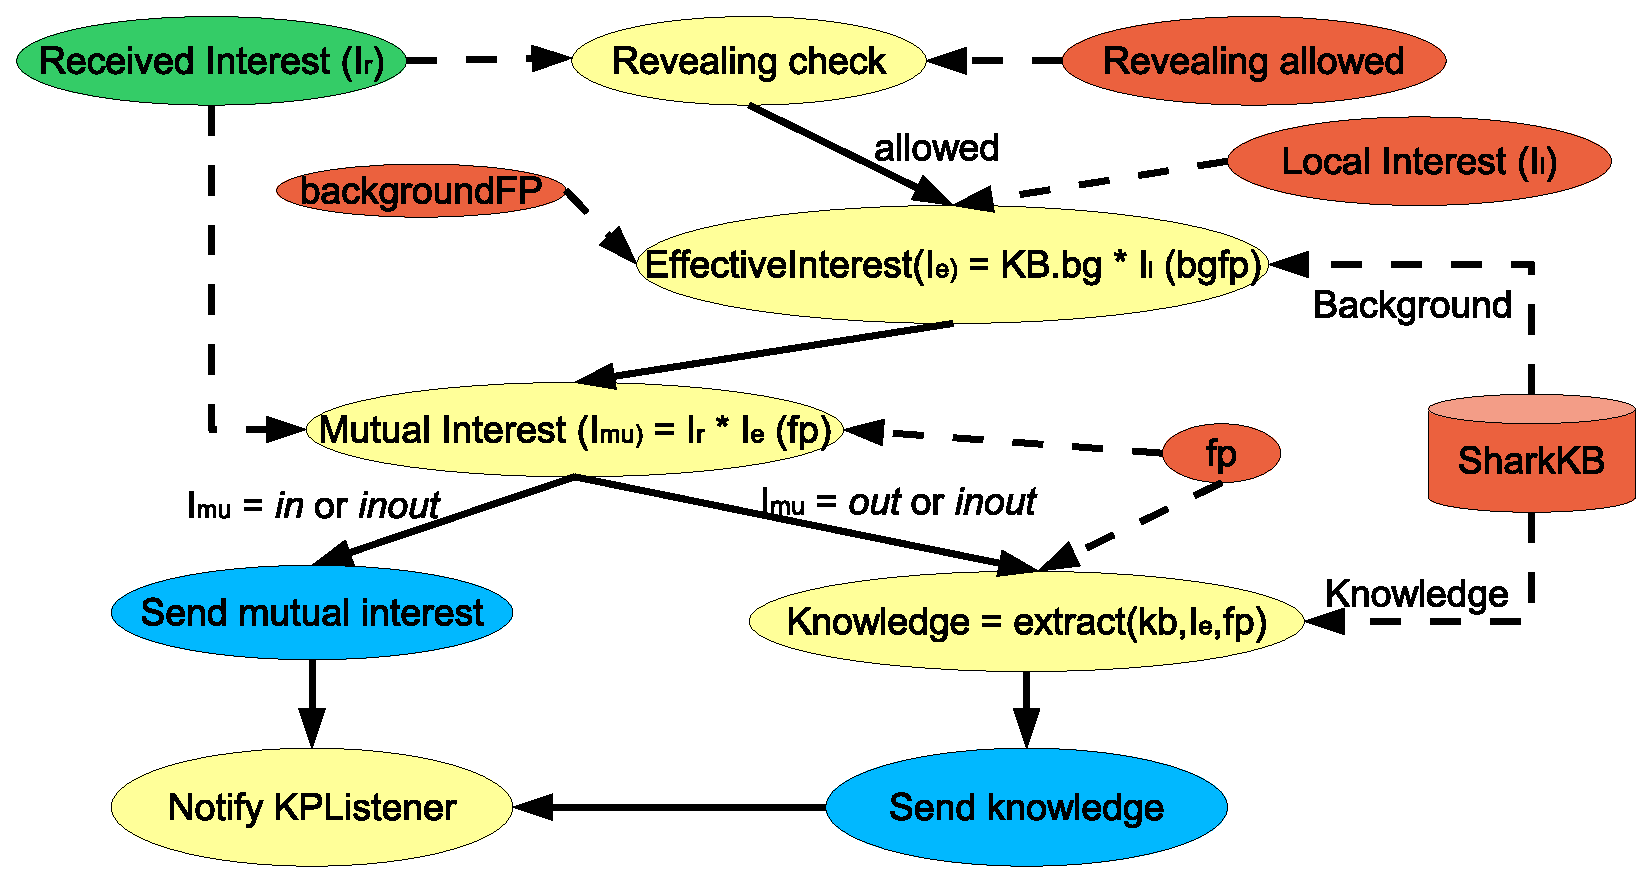
\includegraphics[width=1.00\textwidth]{StandardKP_Expose.eps}
\caption{StandardKP expose algorithm}
\label{fig:StandardKP_expose}
\end{figure}

\paragraph{Effective Interest}
Bob is the remote peer in our example and Alice receives his interest. {\tt StandardKP} calculates the {\it effective interest} by contextualizing the background knowledge with the local interest and some given fragmentation parameters (backgroundFP). What is that good for?

A knowledge base can change. Alice might decide to add information about a Shark application, e.g. {\it SharkNet}. {\it SharkNet} would be a semantic tag and would have a relation to {\it Shark}. Alice has already defined her local interest. She declared her interest to share information about {\it Shark}. What if she wants to share also information regarding SharkNet?

Shark assumes that a local interest can be seen as an anchor. It assumes, that related information shall also be shared automatically to some degree.

The knowledge base background contains the up-to-date vocabulary of each peer. It is taken as source and contextualized with the local interest which serves as context in this case. The {\tt backgroundFP} parameter configures this process. Alice could e.g. define to share sub-topics of {\it Shark} but no super-topics. She could also declare to share nothing that the local interest by setting backgroundFP-{\tt depth} to zero in each dimension.

The result of this calculation is called {\it effective interest}. It can be more general if {\tt backgroundFP} allows fragmentation in some degree. It can only be smaller if {\tt backgroundFP} is zero and tags used in local interest are removed from vocabulary.

Otherwise and in most cases, the {\it effective interest} is larger than or identical to the {\it local interest}.

\paragraph{Mutual Interest}
The received interest is taken and contextualized with the effective interest. Fragmentation parameter (fp) manages this process. This step less complicated than the others. A remote peer, e.g. Bob, showed its interest in communication. The local peer, Alice in this case, calculated her up-to-date interest.

Now she uses Bobs interest as source and finds out what of her interests fits to him. If Bob would be interested in {\it Sports} and she is interested in {\it Shark} no match can be found. If Bob is interested in {\it anything} {\it Shark} would be found as mutual interest, see discussion about revealing several lines above.

The result is called {\it mutual interest}. A mutual interest is assumed to be empty if at least a single dimension could not find a match, see also former section about contextualization of interests.

The process stops if no mutual interest can be found. No message is sent to the other peer. The algorithm is just finished.

\paragraph{Receiving Mutual Interest}
The mutual interest can be a receiving interest which means the direction is either {\tt IN} or {\tt INOUT}. In this case, the mutual interest is send back to the remote peer. Finally, the knowledge port listener are informed about that action.

\paragraph{Sending Mutual Interest}
The mutual interest can be a sending interest which means the direction is either {\tt OUT} or {\tt INOUT}. Knowledge is extracted from the local knowledge base with help of the effective (!) interest and the fragmentation parameter {\tt fp}. Extracted knowledge is sent to the remote peer. Listeners are informed about this action.

\subsubsection{In simple words...}
That was a big deal of details. Nevertheless it was necessary but now we can have a more abstract view on that algorithm.

\begin{itemize}
\item
A peer defines its interest by a {\it local interest}.
\item
It also defines two fragmentation parameter, {\tt backgroundFP} and {\tt fp}.

\item
{\tt backgroundFP} is used to create an up-to-date interest. It take the local interest as anchor and finds related (and maybe new) tags in the vocabulary. This {\it effective interest} can change when peers vocabulary changes.

\item
Effective interest is used to calculate the {\it mutual interest} which comprises things that both peers share. Fragmenation parameter {\tt fp} is used here. It can be assumed that an empty mutual interest is quite common in most applications.

\item
Finally, the mutual interest itself is replied or knowledge that was extracted by means of the mutual interest.
\end{itemize}

Developers should define interest very carefully. Developers can forbid revealing interest and set {\tt depth} to zero in {\tt backgroundFP} or even {\tt fp}. After getting used to those methods, both constraints can be relaxed. But start with the reduced view to be on the safe side. Open your system later step by step when you became familiar with it.

\subsection{constructor and parameters}
The previous process is quite complex. Handling received knowledge is easier. The good point is that we know all parameters which are used in {\tt StandardKP}. The most general constructor is this:

\begin{verbatim}
public StandardKP(SharkEngine se, SharkCS interest,
   FragmentationParameter[] backgroundFP,
   FragmentationParameter[] fp, SharkKB kb) {
\end{verbatim}

\begin{description}
\item[se] is an engine object. Each peer requires a single SharkEngine. It keep all components together. An engine must exist before creating a knowledge port. Engine are discussed in next chapter.

\item[interest] is an interest that defines constraints under which the peer is willing to exchange knowledge.

\item[backgroundFP] is a fragmentation parameter. It is used to update the local interest. In general, it can enhance he rules under which a communication can take place. It takes out the up-to-date background from the knowledge base for this task.

As broader it is defined as more learn peers from each other. Learning and spying are opposite sides of the same coin, though. Developers have to consider how to use it: Being more open, more verbose or more safe, less open. If you have doubts, use {\tt KnowledgePort.getZeroFP()}. It return is parameter that is set to depth 0 and doesn't allow following any relation to other tags in any dimension.

\item[fp] is also a fragmentation parameter. It is used to find mutual interests. Thus, is the parameter which configures how much information get into the knowledge base. {\tt BackgroundFP} configures how much knowledge leaves the peer.

\item[kb] is the a knowledge of this peer. {\tt StandardKP} can changes vocabulary and information depending on parameters and received messages.
\end{description}

There are two other constructor. Here is one:
\begin{verbatim}
public StandardKP(SharkEngine se, SharkCS interest,
  FragmentationParameter[] fp, SharkKB kb) {
    this(se, interest, fp, fp, kb);
}
\end{verbatim}

This constructor can be used of both fragmentation parameters are identical, e.g. {\tt zeroFPs}.

Last one comes here.
\begin{verbatim}
public StandardKP(SharkEngine se, SharkCS interest, SharkKB kb) {
  this(se, interest, KnowledgePort.getZeroFP(),
    KnowledgePort.getZeroFP(), kb);
}
\end{verbatim}

Both fragmentation parameters are set to zero. Changing vocabulary won't have any effect on communication behavior. It is the proposed constructor for beginners. It has no side effects which can arise from an growing vocabulary or added information.

\subsection{doInsert}
{\tt StandardKP} can also process incoming knowledge. The algorithm is less complex than the previous one. Figure \ref{fig:StandardKP_insert} illustrates the steps and used parameter.

\begin{figure}[t]
\centering
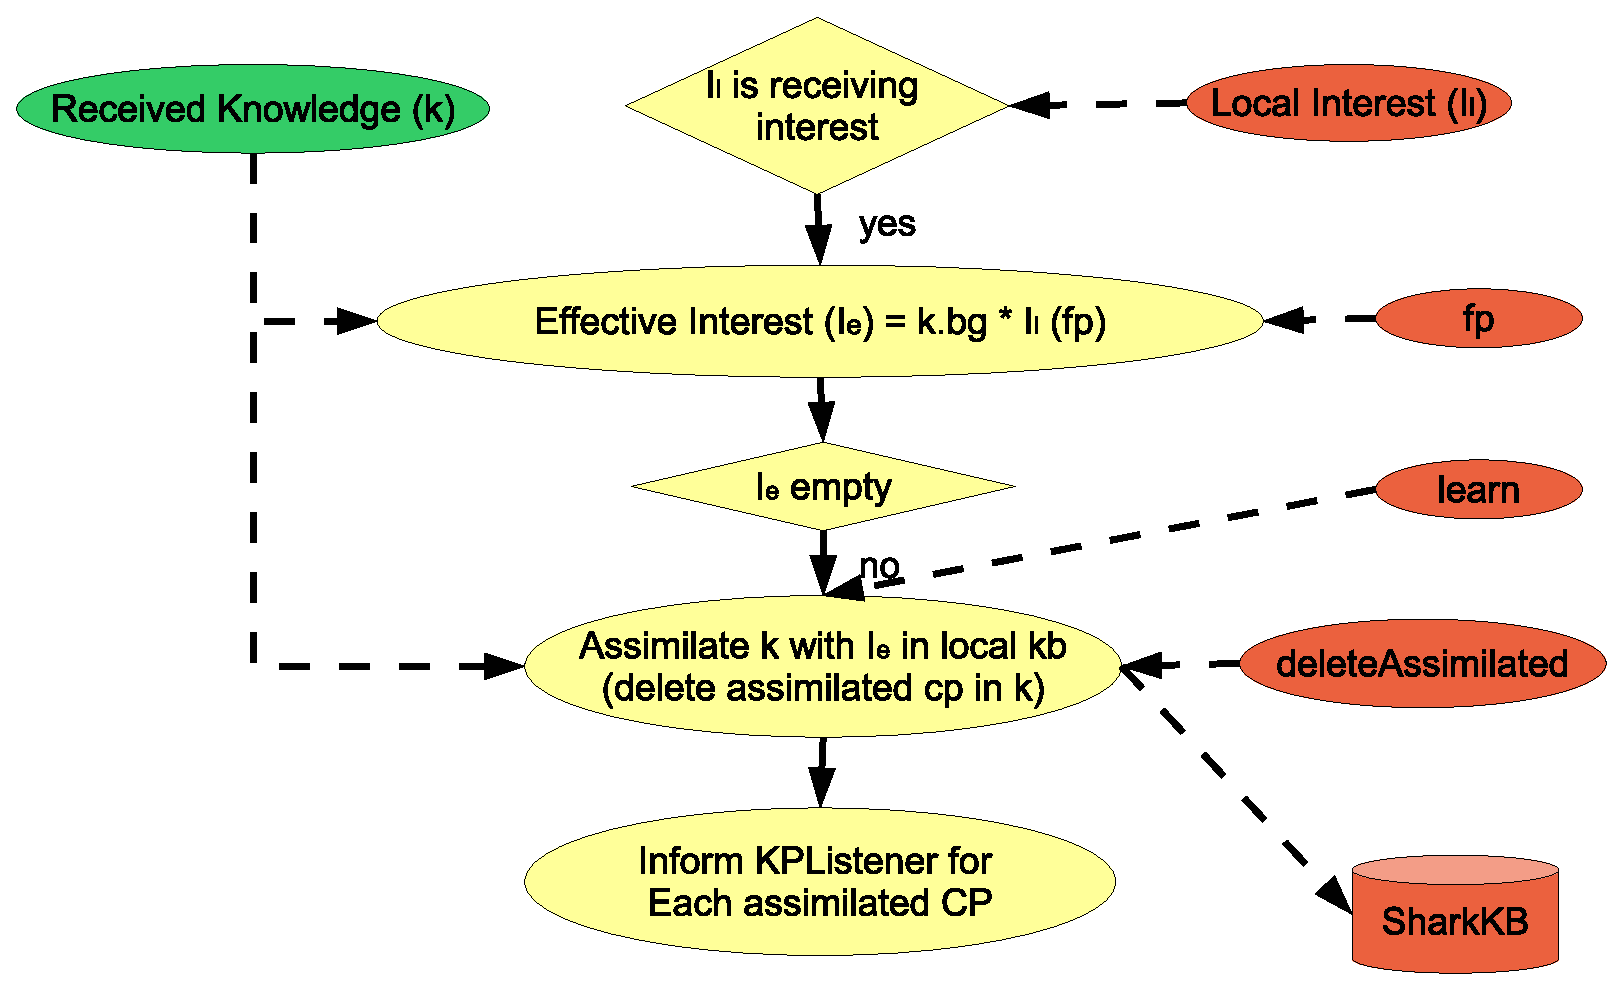
\includegraphics[width=1.00\textwidth]{StandardKP_Insert.eps}
\caption{StandardKP insert algorithm}
\label{fig:StandardKP_insert}
\end{figure}

First of all, it is checked whether the local interest is a receiving interest. More specific, it is checked if the direction is set to {\tt IN} or {\tt INOUT}. We also call such ports {\it IKP - incoming knowledge ports.}. Ports defining their direction with {\tt OUT} are called {\it OKP - outgoing knowledge ports}. A local interests with a direction setting of {\tt INOUT} is both IKP and OKP.
We need an IKP here because knowledge has arrived and there must at least the general interest in receiving something.

Now, vocabulary (in other words:background knowledge) is taken and contextualized with the local interest by means of the fragmentation parameter.
The result is an {effective interest}. It contains tags which are in the knowledge and which also fit to local interest. Thus, the receiving vocabulary is reduced in most cases to tags which fit to peers interests.

The process already ends if the {\it effective interest} is empty. An assimilation process is started otherwise. We have already discussed assimilation in a previous chapters. In short: Each context point is investigated. It is calculated if it fits into the context space defined by the {\it effective interest}. Thus, each, no or some context points can be added to the local knowledge base.

{\tt StandardKP} allows learning of tags. Thus, peers vocabulary grows if context points are assimilated that have unknown tags which are related to known tags. This default behavior can be changed by {\tt learningSTs(false);} Vocabulary remains unchanged in the mode but coordinates of assimilated context points might change.

Assimilated context points are removed from the received knowledge in default. This has, of course, no effect on senders knowledge base. It has an effect on subsequent calls of other knowledge ports, though. They cannot assimilate the same context points again. This default behavior shouldn't be changed in applications with a single knowledge base. It is fully sufficient that one port adds a fitting context point the local knowledge base. Applications using more knowledge bases should consider to change that setting. The default behavior can be changed with {\tt deleteAssimilatedFromKnowledge(false)}.

\subsection{Summary}
{\tt StandardKP} is complex, no doubt about it. But it is complex inside. It can be used quite simple. Developers can start with the easiest constructor and use default settings. Peers will exchange knowledge and learn vocabulary from each other but with less surprises. Our Alice and Bob basic scenario hopefully helps.
It is simple and is neither long nor complex.

Once you have became familiar with it, start experimenting with those fragmentation parameters. It is not complicated but sometimes tricky.

\section{HubKP}
\label{sec:hubkp}
In social groups, a {\it hub} is a person that knows a noteworthy number of other people. A hub is a match maker. In Shark, a hub is a knowledge port that collects and delivers interests of others.

\begin{figure}[t]
\centering
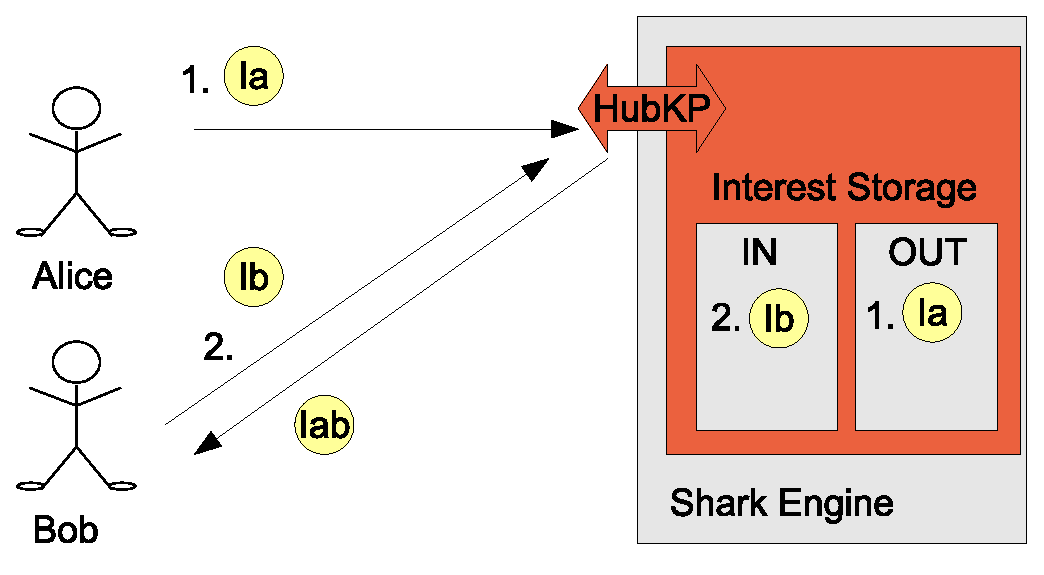
\includegraphics[width=0.70\textwidth]{hubKP.eps}
\caption{HubKP - general idea}
\label{fig:hubKP}
\end{figure}

Figure \ref{fig:hubKP} illustrates an example. There is a SharkEngine on the right. It can run e.g. on a mobile phone. That engine has a running {\tt HubKP} which has its own interest storage. Actually, that storage is separated into a receiving and sending interests.

The little scenario starts with Alice. She is still and always interested in sending information. In our example, she is the first who communicates with that engine. Her interest arrives the engine and is offered to any active knowledge port. {\tt HubKP} becomes active. It hasn't met any other peer and its interest storage is empty. Thus, is just stores the interest and does not reply to Alice.

Bob arrives later and issues his interest. He is still interested in receiving information. The hub takes that interest and stores it as well. Then is calculates: Bob is interested in receiving something. Thus, hub checks its sending interest storage. It takes any interest and calculates the {\it mutual interest}. Non-empty mutual interest are send back as reply. Bob receives a mutual interest of his and Alice interest.

The hub performs the same operation as Bob would do if he would have received that interest from Alice. Even the result is the same. Both mutual interests are identical.

There are differences of course.

\begin{itemize}
\item
A hub helps to bring peers together. Alice and Bob don't have to meet to learn about their mutual interests. Hub collects interests and makes those calculations for other peers.
\item
Peers do not send all their interests to hubs - at least, they shouldn't. A hub runs a peer. Peers can always decide what to expose to whom. A trustworthy friend can know interests of personal matter. An anonymous peer shouldn't.
Thus, when meeting an anonymous hub, peers would send only interests which can be published to literally anybody.
\end{itemize}

That example is perfect to remember the difference between logical and physical sender. In this case, Bob gets a mutual interest. That interest contains a peer in the remote peer dimension. It is Alice. Alice issued her interest in the first place to the hub. Hub just stores the interest and calculates mutual interest after receiving an interest from Bob. The logical sender is Alice. She willingly (or not) stored her interest with the hub.

The physical sender is the hub, though. Thus, Bob can decide how to handle that result. In most cases, it would hurt to handle the result as trustworthy. In this case, Bob would expose a subsequent interest to directly to Alice if he could found her permanent address (e.g. mail address) in remote peer dimension.

Alice would now receive an interest directly from Bob. A direct P2P communication is established now and End-to-End-Security could be established.

This book to teach programming with Shark. Therefore, we have a look into the implementation. Source code can be found in our open software repository. Visit our web page where to find our repository. (It was Projekt SharkFW on GitHub when this chapter was written).

\subsection{Usage}
Usage of the hub port is very simple. Once a {\tt HubKP} is instanciated on a {\tt SharkEngine} it offers hub features to other peers.

\begin{verbatim}
SharkEngine se = ... // was created earlier in code

KnowledgePort hub = new HubKP(se, 3600);
\end{verbatim}

Two features are to be noted:

\begin{enumerate}
\item
This hub implementation has no persistent memory. All stored interest get lost if the port or the whole engine terminates. It's a feature. Hub is not (yet) intended to be a permanent kind of directory for peer interests.
\item
Second parameter describes lifetime of interest in the hub storage. In this example, interest are forgotten after 3600 seconds which is one hour.
\end{enumerate}

\subsection{Implementation}
We won't explain each line of code but the core parts of the class. Nevertheless, the whole implementation has 145 lines of code with comment lines.
If you are curious - have a look into our source code repository.

{\tt HubKP} has to implement the {\tt doInsert} method. This method is abstract in class {\tt KnowledgePort} and {\tt HubKP} must have an implementation to become a non-abstract class. The implementation is empty, though:

\begin{verbatim}
@Override
protected void doInsert(Knowledge k, KEPConnection responseFactory) {
     // Do nothing. We don't process inserts.
}
\end{verbatim}

A hub does not deal with information but with interests. There is nothing to do for it when receiving information.

It implements {\tt doExpose}. The following code was copied from
the repository. Some unimportant lines and comments are removed to
spare space.

\begin{verbatim}
protected void doExpose(SharkCS interest,
                        KEPConnection kepConnection) {
  try {
    // process interest
    if(interest.getDirection() == SharkCS.DIRECTION_IN ||
        interest.getDirection() == SharkCS.DIRECTION_INOUT) {

       this.doProcess(interest, kepConnection, this.outInterests);
   }

   if(interest.getDirection() == SharkCS.DIRECTION_OUT ||
       interest.getDirection() == SharkCS.DIRECTION_INOUT) {

       this.doProcess(interest, kepConnection, this.inInterests);
   }
  }
  catch(SharkException e) {
   L.l("failure while processing interest in HubKP.);
  }

  // finally save it
  if(interest.getDirection() == SharkCS.DIRECTION_IN ||
       interest.getDirection() == SharkCS.DIRECTION_INOUT) {

      this.inInterests.addInterest(interest);
  }

  if(interest.getDirection() == SharkCS.DIRECTION_OUT ||
       interest.getDirection() == SharkCS.DIRECTION_INOUT) {

      this.outInterests.addInterest(interest);
  }
}
\end{verbatim}

There are just two parts in method implementation. First, it is checked whether received interest is a receiving interest (direction is IN or INOUT) or a
sending interest (direction is OUT or INOUT). An interest with INOUT in its direction is both and is handled twice.

The method doProcess is called with the received interest, {\tt kepConnection} and the appropriate interest storage. {\tt outInterests} contains received sending interests. They could match with an receiving interest and vice versa.

The second part stores received interest in its storage. Again, an INOUT interest is stored in both storages.

That's not really difficult. Neither is {\tt doProcess}:

\begin{verbatim}
private void doProcess(SharkCS interest,
                       KEPConnection kepConnection,
                       InterestStore storedInterests)
                  throws SharkKBException, SharkException {

  Iterator<SharkCS> interestIter = storedInterests.getInterests();

  while(interestIter.hasNext()) {
      SharkCS storedInterest = interestIter.next();

      // mutual interest?
      Interest mutualInterest = SharkCSAlgebra.contextualize(
          storedInterest, interest, fps);

      if(mutualInterest != null) {
          kepConnection.expose(mutualInterest);
      }
  }
}
\end{verbatim}

{\tt doProcess} is called with the received interest and a storage of already stored interests which could fit. {\tt kepConnection} is required to reply.

First, an iterator is created that iterates any stored interests. Variable
{\tt storedInterest} refers to an stored interest in each loop. A mutual interest is created for each combination (received and stored interest).
A non-empty mutual interest indicates both peers have something in common: The peer that was just met and the peer from which hub had stored its interest.

The action is straightforward: A non-empty mutual interest is exposed to
the peer that issued its interest. In our previous example, the hub would find Alice interest in its storage and send Bob the non-empty mutual interest.

That's it. We won't discuss the interest storage implementation. It organizes removal of outdated interests. That's no rocket science. Have a look into the code.

We are ready with {\tt HubKP}. It isn't difficult, is it? Let's have a look on a sketch of a chat implementation with knowledge ports.

\section{ChatKP}
\label{sec:chatkp}
A chat is a pretty simple distributed system. A peer creates a message and wants it send to a recipient. Recipient shall read the message and can reply. This principle has to translated into the Shark concept. And this easy.

\begin{figure}[t]
\centering
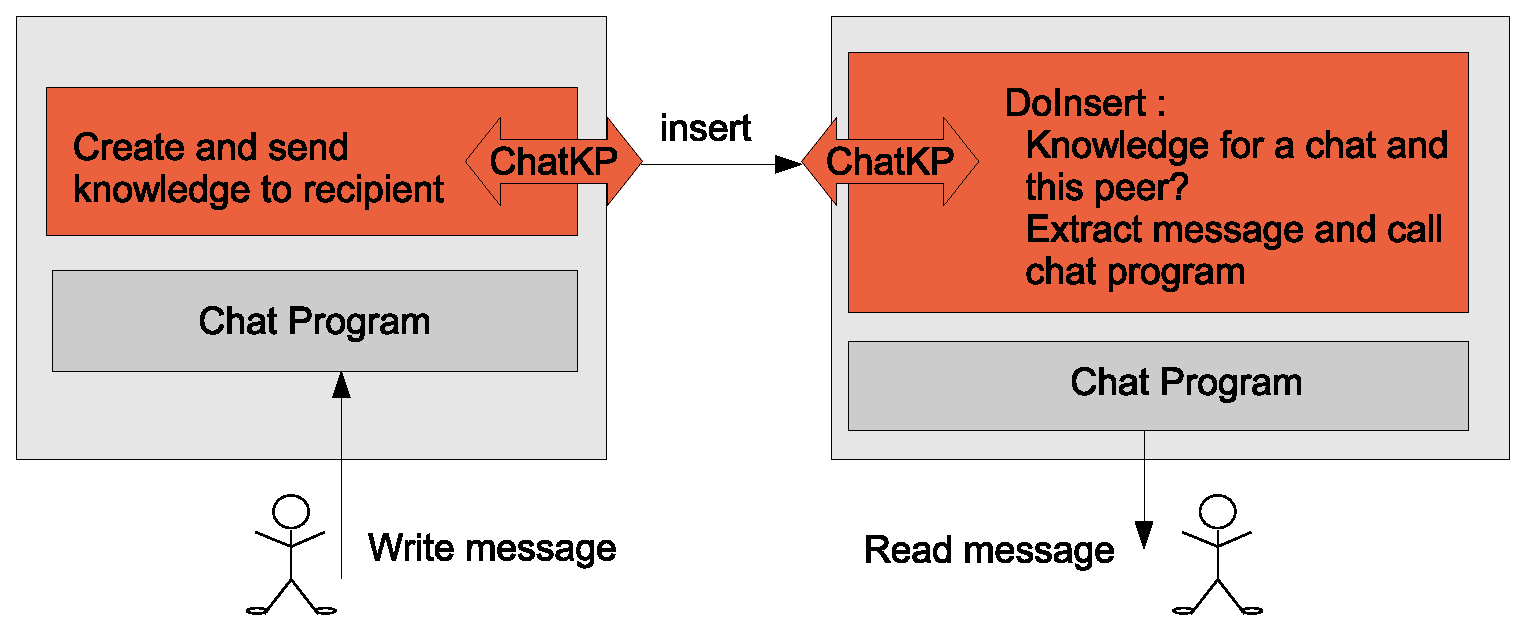
\includegraphics[width=0.90\textwidth]{chatKP.eps}
\caption{ChatKP - general idea}
\label{fig:chatKP}
\end{figure}

Figure \ref{fig:chatKP} illustrates (one possible) concept of a chat implementation with Shark. There is a user creating a message in the lower left corner. The message is written with a chat program. The message is transmitted to a {\tt ChatKP}.

There are two data types in Shark which can be transmitted, interests and knowledge. The ''natural'' choice is wrapping the message into knowledge. Why is it ''natural''? A message is an arbitrary number of bytes. That is the definition of information in Shark. Information are transmitted inside knowledge. That's the reason.

{\tt ChatKP} creates knowledge which comprises several steps. First, a context point is created. It coordinates must be defined. In this implementation, the topic is set to a pre-defined semantic tag named {\it chat} and a unique subject identifier. Originator and peer is the creating peer. Remote peer is the recipient of that message. Multiple message are to be created for multiple recipients.

Knowledge is send to the recipient. A {\tt ChatKP} must be in place. It takes each incoming knowledge. It checks: Does this knowledge contain context point with a topic {\it chat}? Is it issued from an allowed peer? Is the receiving peer the intended recipient? If so, information from the context point can be extracted. The job of {\tt ChatKP} ends here. It isn't its job to interpret the message or interact with a user. It calls the local chat program to deal with the newly arrived message.

{\tt ChatKP} implementation is just a sketch but no ready for usage in a productive environment. There is no section {\it ChatKP usage} for that reason.

\subsection{Implementation}

\begin{figure}[t]
\centering
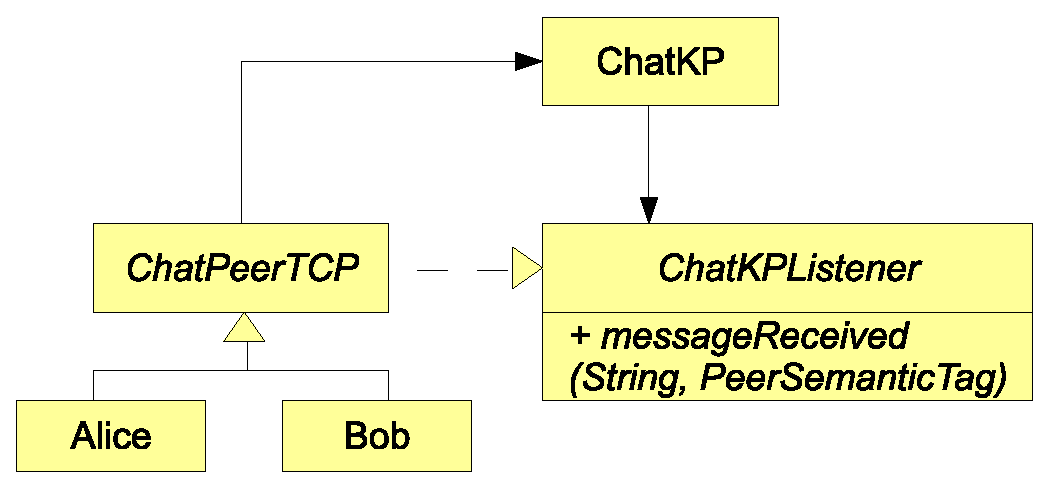
\includegraphics[width=0.70\textwidth]{chatClassDiagram.eps}
\caption{Chat implementation (sketch) - class diagram}
\label{fig:chatClassDiagram}
\end{figure}

Chat implementation is made up by four classes and one interface, see figure \ref{fig:chatClassDiagram}. {\tt ChatKPListener} is an interface that declares a single method: {\tt messageReceived}. This method is called by a {\tt ChatKP} whenever a new message arrived the peer. It has two parameters. First parameter is the actual message. Second parameter contains the sender. Later in this section we will have a look into {\tt ChatKP} implementation.

We have implemented an abstract class {\tt ChatPeerTCP}. It is abstract because is does {\it not} implement {\tt messageReceived}. Implementations are made in Alice and Bob. We start with Alice:

\subsection{Alice}

\begin{verbatim}
public class Alice extends ChatPeerTCP {

  public Alice(String peerName, String peerSI,
               String address, int port)
               throws SharkProtocolNotSupportedException, IOException {
    super(peerName, peerSI, address, port);
  }
\end{verbatim}

Alice extends {\tt ChatPeerTCP} which has a constructor that expects necessary data to describe a peer. Those data are: name of the peer, subject identifier, address and port. The final parameter already indicates: {\tt ChatPeerTCP} only uses TCP as protocol. As already noted - this program is a sketch but can be extended which is an exercise in this chapter.

The main method brings no surprises:
\begin{verbatim}
  public static void main(String[] args)
    throws SharkProtocolNotSupportedException, IOException {
    // setup alice peer
    Alice alice = new Alice("Alice",
                            "http://www.sharksystem.net/alice.html",
                            "tcp://localhost:7070",
                            7070
     );

    System.out.println("Alice is running - start Bob now");
  }
}
\end{verbatim}

An object of class {\tt Alice} is created. Alice is described by the name ''Alice'' and her - now well-known - subject identifier. We use a local TCP address with port 7070. Note again: That program will run only on a single computer. It requires some (little) extensions to make it real chat.

Finally, we have a look at the {\tt messageReceived} implementation:
\begin{verbatim}
  @Override
  public void messageReceived(String message, PeerSemanticTag sender)
                    throws SharkException, IOException {
    System.out.println("Alice has got that message:\n" + message);
    System.out.println("\nfrom:\n" + L.semanticTag2String(sender));
    System.out.println("Alice is going to reply with \"Hi Bob\"\n");
    this.chatKP.sendMessage("Hi Bob");

    // end of communication
    this.stop();
  }
\end{verbatim}

The first three lines just print out the fact that a message was
received and from whom. Afterwords, a message (''Hi Bob'') is send
back. Apparently, a real chat program must prompt users entering
a reply. Finally, {\tt this.stop()} is called which is implemented in
{\tt ChatPeerTCP} and simply stops TCP communication in general. Thus,
Alice sends a reply and shuts down whenever she receives a single message.
It is a sketch but illustrates the principle. The more interesting part are
implemented in {\tt ChatKP} anyway. But first have a look at the Bob implementation.

\subsection{Bob}
\begin{verbatim}

public class Bob extends ChatPeerTCP {

  public Bob(String peerName, String peerSI, String address, int port)
             throws SharkProtocolNotSupportedException, IOException {
    super(peerName, peerSI, address, port);
  }
\end{verbatim}

The constructor is identical with Alice. It feeds the {\tt ChatPeerTCP} constructor.

\begin{verbatim}
  @Override
  public void messageReceived(String message, PeerSemanticTag sender)
                              throws SharkException, IOException {
    System.out.println("Bob has received something:\n" + message);
    System.out.println("\nfrom:\n" + L.semanticTag2String(sender));

    // end of communication
    this.stop();
  }
\end{verbatim}

Bob peer can receive a message. It is just printed out and communication is stopped. We already know Alice' behavior. She would send a message as soon as she has got one from Bob and terminate. Bob waits for a message and terminates without further actions.

\begin{verbatim}
  public static void main(String[] args)
    throws SharkProtocolNotSupportedException, IOException,
           SharkException, InterruptedException {

    System.out.println("Alice must run first");
    Bob bob = new Bob("Bob",
                      "http://www.sharksystem.net/bob.html",
                      "tcp://localhost:7071",
                      7071
    );

    System.out.println("Bob started - send message to Alice");

    PeerSemanticTag alice = InMemoSharkKB.createInMemoPeerSemanticTag(
                            "Alice",
                            "http://www.sharksystem.net/alice.html",
                            "tcp://localhost:7070");

    // send first message
    bob.chatKP.sendMessage("Hi Alice", alice);
  }
}
\end{verbatim}

A Bob object is created in main method. It uses port 7071. Bob creates a peer description for Alice which is required to call {\tt sendMessage()}. The final line asks {\tt chatKP} to send ''Hi Alice'' to the peer listening at port 7070 on localhost.

The example works if the Alice program was started first. Alice would wait for incoming messages. Bob would send a message within its main method. Alice would get it, reply immediately and terminate. Bob would receive a reply print it out and stop working.

Lets have a look into {\tt ChatPeerTCP}.

\subsection{ChatPeerTCP}
\begin{verbatim}
public abstract class ChatPeerTCP implements ChatKPListener {
  private SharkEngine se = null;
  protected final ChatKP chatKP;
\end{verbatim}

That class implements a stand-alone program. It keeps a shark engine
and a {\tt ChatKP} as private member. Both are initialized in the
constructor we already know:

\begin{verbatim}
  public ChatPeerTCP(String peerName, String peerSI,
                     String address, int port)
                      throws SharkProtocolNotSupportedException,
                             IOException {

    this.se = new J2SEAndroidSharkEngine();

    // create PeerSemanticTag describing peer itself
    PeerSemanticTag peer = InMemoSharkKB.createInMemoPeerSemanticTag
                           (peerName,
                            peerSI,
                            address);

    // create chat kp
    this.chatKP = new ChatKP(this.se, peer);

    // subscribe to news
    this.chatKP.addListener(this);

    // start listening at address - can throw exceptions
    this.se.startTCP(port);
  }
\end{verbatim}
We have already seen that Alice and Bob described themselves with
name, subject identifier and so forth. The constructor takes those parameters.
It creates a shark engine first. Second, a peer semantic tag is created that describes the peer itself (Alice or Bob in our example). Third, an object of
{\tt ChatKP} is created. It takes two parameters: Engine and peer that runs that
engine. Fourth, the objects subscribes to {\tt ChatKP} as listener. This call informs {\tt ChatKP} to call {\tt messageReceived} (implemented in Alice and
Bob). Finally, the TCP connection is started. Now, the engine is listening at the defined port. It will receive incoming KEP message and transmit them to all active knowledge ports. In this program there is only one: {\tt ChatKP}.

\begin{verbatim}
  public void stop() {
    this.se.stop();
  }
}
\end{verbatim}
The final lines in this class implement the stop method. It is very simple. {\tt stop} in shark engine is called. The engine stops listening at any protocol. Open sessions remain unharmed, though.

\subsection{ChatKP}
Most work is done in {\tt ChatKP}. It can be re-used in productive programs.
We are going to skip some trivial parts of the program. The whole implementation can be found on Shark tutorials web page.

\begin{verbatim}
public class ChatKP extends KnowledgePort {
  public static final String CHAT_TOPIC_SI =
    "http://www.sharksystem.net/examples/chat/chatinterest.html";
  private PeerSemanticTag remotePeer = null;
  private ChatKPListener listener = null;
  private final PeerSemanticTag owner;

  public ChatKP(SharkEngine se, PeerSemanticTag owner) {
    super(se);
    this.owner = owner;
  }

  @Override
  protected void doExpose(SharkCS interest, KEPConnection kepConnection) {
  }
\end{verbatim}

{\tt ChatKP} is a {\tt KnowledgePort} and has to call its constructor
({\tt super(se);}). The engine object already exists and is transmitted as
parameter in its constructor. Some private member are declared.
{\tt CHAT\_TOPIC\_SI} was defined as unique identifier for that chat implementation. It will be used in the topic dimension to create knowledge that can be send to another peer. {\tt remotePeer} will contain the peer with whom a chat will established. {\tt listener} will contain the chat program to which incoming messages are to be propagated. {\tt owner} is the peer that runs that chat.

That knowledge port does not handle interest. {\tt doExpose()} contains no action. That makes sense since whole message exchange is mapped on exchanging knowledge between peers.

Teh {\tt doInsert} makes the job:
\begin{verbatim}
  @Override
  protected void doInsert(Knowledge k, KEPConnection kepConnection) {
    Enumeration<ContextPoint> cpEnum = k.contextPoints();

    if(cpEnum != null) {
      ContextPoint cp = cpEnum.nextElement();
      ContextCoordinates cc = cp.getContextCoordinates();
      SemanticTag topic = cc.getTopic();
      if(!SharkCSAlgebra.identical(topic, this.getChatTopic())) {
        // this knowledge is not about chatting
        return;
      }

      PeerSemanticTag rPeer = cc.getRemotePeer();
      if(!SharkCSAlgebra.identical(rPeer, this.owner)) {
        // remote peer does not want to talk to me
        return;
      }

      // remember that sender
      PeerSemanticTag peer = cc.getPeer();
      this.remotePeer = peer;

      // seems to be a chat message in knowledge - unwrap
      Iterator<Information> infoIter = cp.getInformation();
      if(infoIter != null) {
        String message;
        try {
          message = infoIter.next().getContentAsString();

          // notify listener about new message
          this.messageReceived(message, peer);
        } catch (Exception ex) {
        }
      }
    }
  }
\end{verbatim}

This method is called whenever knowledge reached that peer. First, it is tested if at least a single context point is present in the knowledge object. Second, it is tested if this context point is about ''chatting''. If not, the port aborts that algorithm. That knowledge has nothing to do with a chat.

Second, it is tested whether this peer is recipient of this chat message. Third, it is tested of the remote peer fits to accepted remote peers by this peer.

Information objects are extracted from the context point if all tests are passed. That message is transformed into a string an send to chat programs who have subscribed before. That's performed via {\tt this.messageReceived}.

Let's have look into this implementation:
\begin{verbatim}
  private void messageReceived(String message, PeerSemanticTag sender)
                               throws SharkException, IOException {
    if(this.listener != null) {
      this.listener.messageReceived(message, sender);
    }
  }
\end{verbatim}

It's straightforward. A listener is called if a listener has be subscribed. We don't present subscribing implementation here. It is very simple.

Now, we have seen how {\tt ChatKP} handles incoming chat messages. Now we have to learn how it sends messages.

\begin{verbatim}

  public void sendMessage(String message, PeerSemanticTag recipient)
                          throws SharkException, IOException {

    // first create coordinates
    SemanticTag chatTopic = this.getChatTopic();
    ContextCoordinates cc = InMemoSharkKB.createInMemoContextCoordinates(
                              chatTopic, // its a chat message
                              this.owner, // originator is owner of engine
                              this.owner, // peer is owner as well
                              recipient, // want to talk with connected peer
                              null, // time and place is irrelevant
                              null,
                              SharkCS.DIRECTION_OUT
                             );

    // all metadata set - lets create a context point
    ContextPoint cp = InMemoSharkKB.createInMemoContextPoint(cc);

    // add message
    cp.addInformation(message);

    // create knowledge
    Knowledge k = InMemoSharkKB.createInMemoKnowledge();

    // add context point
    k.addContextPoint(cp);

    // send to remote peer
    this.sendKnowledge(k, recipient);
  }

  private SemanticTag getChatTopic() {
    SemanticTag chatTopic = InMemoSharkKB.createInMemoSemanticTag(
                              "ChatTopic",
                               ChatKP.CHAT_TOPIC_SI);
    return chatTopic;
  }
}
\end{verbatim}

This message takes two parameter: message and recipient. This message has two wrap the message into a knowledge object. First, context coordinates are required. Seven parameter are required.

The topic is created with {\tt getChatTopic}. See also the method implementation. A semantic tag is created labeled with ''ChatTopic''. It semantics is defined by {\tt CHAT\_TOPIC\_SI}, see above.

Originator and peer dimension is set to the owner of this engine. This makes
perfectly sense because this peer is creator and sender of the message.

Remote peer is set to the recipient which is parameter of this method.

Location and time dimension remains empty. Spatial and temporal constraints are not necessary for this application.

Direction is set to {\tt OUT} because we are going to send something out.

A context point is created with those coordinates. The chat message can be attached as information. A knowledge object is created and the context point is added. Finally, that knowledge object is send out to the recipient peer with
{\tt sendKnowledge(k, recipient)}.

The receiving peer would get a knowledge object via KEP-insert and call {\tt doInsert} on all active knowledge ports. We have already seen the {\tt ChatKP} implementation.

That's it. Download the chat program from our web page and let it run. Don't forget to run Alice first. Try to understand the program. Make it a real chat program afterwards, see also the exercises section in this chapter.

\section{Exercises}

\begin{enumerate}
\item
Re-implement KP from last chapter but use {\tt StandardKP} as basis instead abstract class {\tt KnowledgePort}.
\item
Extend {\tt ChatKP} to make it a real chat program.
\end{enumerate}

\chapter{Shark Engine}
\label{sec:sharkengine}

\section{Architectur}
Figure \ref{fig:sharkComponents} illustrates the major components which are discussed in a little more detail in this section.

\begin{figure}[t]
\centering
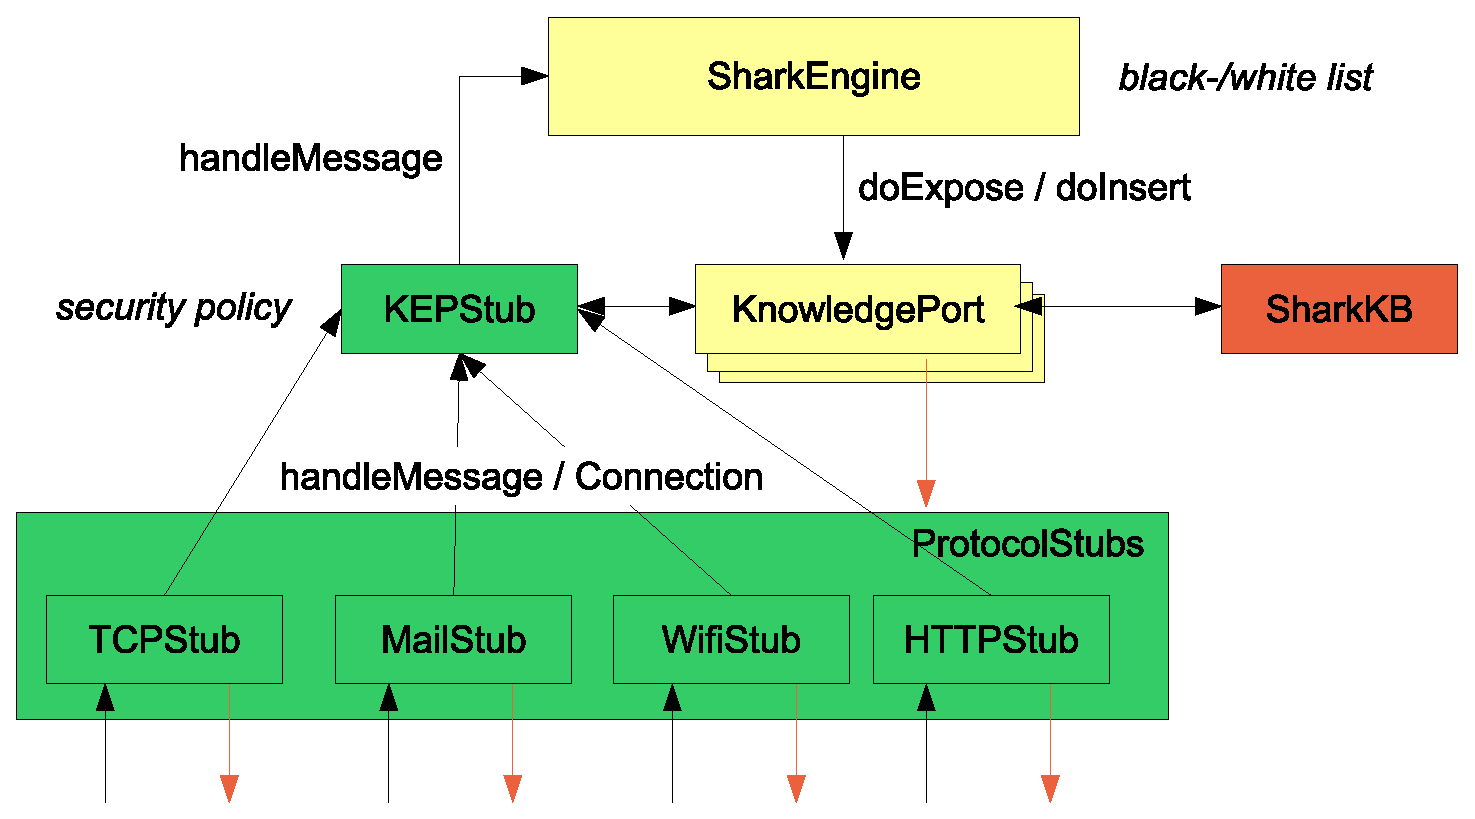
\includegraphics[width=1.00\textwidth]{sharkComponents.eps}
\caption{Shark components}
\label{fig:sharkComponents}
\end{figure}

\subsection{Stubs}
Let's start with the {\it protocol stubs}. Shark supports TCP and E-Mail in version 2. HTTP will be supported soon\footnote{which is quite simple because HTTP is actually a TCP stub with an additional HTTP header} and Wifi-Direct which is already working in the laboratory but requires further tests to be officially added to the system.

Each stub is actually protocol server and client. The TCP stub supports e.g. a method to send data to another peer via TCP. The same stub comprises a TCP server as well which accepts new connections. Developers won't get bothered with those details anyway.

Server parts of each stub just receives messages (e.g. with POP3) or establish connection (TCP and Wifi). Management of this data and connections is handled by the {\it KEP Stub}.

The {\it KEP stub} takes data from underlying protocols and tries to parse a KEP message. It decrypts messages and verifies signatures if required and checks if message comply with defined security policies (which are explained in chapter \ref{sec:security}). Parsing and security methods can fail. {\it KEP stub} writes a log messages and throws any data away. Valid KEP messages are given to the {\it SharkEngine}. 

\subsection{SharkEngine}
The engine has a very little job in KEP message handling. Developers can maintain black- and white lists in the engine. Only KEP messages from allowed senders are accepted. All others are simply dropped without further actions.

The engine also keeps a list of active knowledge ports. The engine checks whether the KEP message contains an {\it interest} or {\it knowledge} and calls {\tt doExpose} or {\tt doInsert} on each active knowledge port.

\subsection{Knowledge Port}
We have already discussed knowledge ports and their usage. The can work with a local knowledge base. Knowledge ports can reply to the sender. In most cases, an already established connection is used. Knowledge ports can also decide to send messages to other addresses. In this case, the KEP stub is used to create a new connection. Developers are not aware of using KEP stub or protocol stubs. They just use the {\tt KEPConnection} interface.

\subsection{Message2StreamStub}
{\it Interest} are usually small in terms of number of bytes. {\it Knowledge} can be huge. Huge data is no problem in general when using a stream protocol like TCP. It becomes a problem when using message oriented protocols like e-mail. 

We had serious discussions how to deal with that problem. An e-mail has a limited length. It depends on capacity and policy of recipient's mail server. What can be done if a KEP message exceeds that limit? In general, there are two possible way:

\begin{enumerate}
    \item Throwing an exception. That would make the framework easier to implement. Unfortunately, developers would be responsible to ensure that KEP message has a maximum size.
\item The framework solves that problem. 
\end{enumerate}

We have chosen the second option. Developers can ignore length of KEP message or send knowledge. There is the {\tt Message2StreamStub} class inside the framework. It takes a message based protocol like SMTP and makes it usable as a stream protocol. It makes a little flow control. The principle is simple: KEP messages which exceed the maximum message length are split into $n$ messages. Each message gets its own number beginning with 0 and the maximum number. Recipients acknowledge received messages which triggers the next package. Developers don't have to care about this little flow control. The behavior can be visited by observing mailboxes used by peers.

In any case, large data are only transmitted via e-mail if no other protocol is available. Its throughput is awful. We come back to that point in section \ref{sec:se:protocolPriorities}

\section{Knowledge Port Management}
Knowledge ports are managed by the Shark engine. Developers don't have to add a knowledge port to the engine. It is done by the {\tt KnowledgePort} constructor.

Each constructor requires at least a Shark engine as parameter. There was e.g. this line in our Alice program:

\begin{verbatim}
SharkEngine aliceSE = ...;
StandardKP kp = new StandardKP(aliceSE, cc, aliceKB);
\end{verbatim}   

The constructor adds the port to the engine. Knowledge ports can be deleted:

\begin{verbatim}
aliceSE.deleteKP(kp);
\end{verbatim}

Object {\tt kp} is removed from the list of knowledge ports. It cannot be added. The only way is to create a new knowledge port with same parameters. Knowledge ports can be activated and deactivated. That's a feature of knowledge ports, see section \ref{sec:knowledgePorts}.

All knowledge ports can be retrieved.
\begin{verbatim}
aliceSE.getAllKP();
\end{verbatim}

\subsection{Publishing}
Each engine offers methods to start or re-start a conversion between peers.
Let's have a look at the following code.

\begin{verbatim}
PeerSemanticTag remotePeer = ...;
aliceSE.publishKP(kp, remotePeer);
\end{verbatim}

Engine takes the interest which is stored in the knowledge port. This interest is sent as {\it KEP expose} to {\tt remotePeer}.

\begin{verbatim}
aliceSE.publishKP(kp);
\end{verbatim}

This method is similar to the previous version. Recipients are extracted from {\tt kp} interest: Each peer {\it remote peer dimension} gets an expose message.
Apparently, it only works if this dimension is not empty.

\begin{verbatim}
aliceSE.publishAllKP(remotePeer);
\end{verbatim}

This method publishes any knowledge port to {\tt remote peer}.

\begin{verbatim}
aliceSE.publishAllKP();
\end{verbatim}

This method iterates over all knowledge ports and performs an {\tt publishKP(kp)} on each of them.

\section{KEP communication}
\label{ref:sec:KEP}
We have already seen that {\tt KEPStub} orchestrates communication and hides protocol specifics and security algorithms from developers. {\tt KEPStub} provides several other, maybe, useful methods which are discussed in this chapter. 

Developer don't have to access {\tt KEPStub} directly. Shark engine acts as {\it facade}: It offers methods and delegates parts of their duties to other components. Thus, sometime we might intermix {\tt KEPStub} and {\tt SharkEngine} in the next section. Don't care: Any method is available on the {\tt SharkEngine} interface. Internals are of no interest for Shark application developers.

\subsection{Communication History}
Peers send and receive messages. Received message can be handled by knowledge ports or not. The later are called {\it unhandled messages}. Sending can fail. Shark is meant to be a framework for spontaneous networks. Communication breakdown must be seen as usual event and not as avoidable error. Messages that are ought to be sent are stored and can be re-sent later.

The following methods are offered by {\tt SharkEngine}.

\begin{verbatim}
// returns all interests exposed since a given point in time
Iterator<SharkCS> getSentInterests(long since);

// returns all knowledge sent since a given point in time
Iterator<Knowledge> getSentKnowledge(long since)
  
// returns interests which are not handled by any knowledge port
Iterator<SharkCS> getUnhandledInterests(long since)

// returns background knowledge of knowledge that wasn't handled by
// any knowledge prt
Iterator<SharkCS> getUnhandledKnowledge(long since);
\end{verbatim}

First three methods are obvious. {\tt getUnhandledKnowledge} returns a context space but no knowledge. That's because of resource considerations. Knowledge tends to be huge. Context spaces are quite small compared to knowledge. Knowledge arrives with {\it KEP insert}. Active knowledge ports have the chance to assimilate that knowledge. The engine stores the background knowledge of non-assimilated knowledge but not knowledge itself. Background knowledge contains any necessary information to get that knowledge again. Thus, applications could iterate non-assimilated background knowledge and issue {\it KEP expose} requests to the other peers which can re-sent that knowledge.

\subsection{Silent period and empty knowledge}
{\tt KEPStub} keeps track of sent interests and knowledge. It checks whether 
or not those messages were already sent and sometimes prevents the system from sending. 
It is a very useful feature especially for spontaneous networks which tend to stutter. Let's explain it by an example:

We are familiar with the Alice and Bob basic communication scenario. Imagine that applications runs on mobile phones which communicate solely with Wifi-direct. Alice and Bob e.g. meet at a table having lunch. Their devices establish a connection. At least one device issues an interest after a connection establishment. The communication takes place - anything it fine.
Imagine, Bob stands up e.g. to go for some tomato sauce. Wifi communication breaks down more or less immediately. It is re-established when he comes back.
Thus, one peer would issue the same interest as minutes before, both devices would perform same communication again and again. That additional power consumption would be a heavy burden for mobiles phones accumulator.

There is a {\it silent period}. {\tt KEPStub} don't issues identical KEP messages within that silent period. Identical means identical content and identical recipient. When Bob returns, one device might prepare for sending the same interest again but {\tt KEPStub} would prevent from sending that message.

That period can be set.
\begin{verbatim}
public void setSilentPeriod(int milliseconds);
\end{verbatim}

There is a default setting defined in {\tt DEFAULT\_SILTENT\_PERIOD}.

Nevertheless, it is useful to re-expose interests to other peers. That's what we do when we read or listen to our preferred news paper / channel. Maybe the other peer has new information.

{\tt KEPStub} keeps track of delivered knowledge. Identical knowledge won't be sent again. {\tt KEPStub} uses a history for that reason which can be removed.

\begin{verbatim}
// removes expose and insert history
removeSentHistory();
\end{verbatim}
Afterwards, the system has forgotten its history and would send any knowledge.

There is a final quite special scenario. 
We have discussed {\tt StandardKP}. Received interests are pre-processed. Finally, they are used to extract knowledge from the local knowledge base. {\tt KEPStub} prevents re-sending knowledge which keeps resource on both sides.
Thus, {\tt KEPStub} investigates any knowledge that is to be sent. Information that has already been delivered to the recipient is removed. Information can be removed during that process. It can also happen that all information is removed. In this case, no knowledge would be sent at all.

Some applications might not be happy with that behavior. They might want to get a reply even if there exists no new information. Their is a compromise. {\tt KEPStub} can be set to allow sending {\it empty} knowledge.

\begin{verbatim}
public void setAllowSendingEmptyContextPoints(boolean allowed);
\end{verbatim}

If {\tt allowed} is set to {\tt true}, knowledge is sent even if any information was stripped of before. Thus, recipients would get background knowledge without information. {\tt StandardKP} would do nothing with it. Other ports might take is as {\tt still-alive-message} or might assimilate the semantic tags. It is up to the applications.

Default setting is {\tt false}. Empty knowledge won't be sent.

\subsection{Some other protocol methods}
We have already seen examples for starting a stopping protocol stubs. 
There are others. They follow a simple strategy. But have a look at the
declaration (which can also be found in {\tt SharkEngine}).

\begin{verbatim}
// start Mail if available
public void startMail()
   throws SharkProtocolNotSupportedException;

// start TCP if available
public void stopTCP() 
   throws SharkProtocolNotSupportedException;

// start WifiDirect if available
public void stopWifiDirect() 
   throws SharkProtocolNotSupportedException;


// convenient: start any available protocol
public void start() throws IOException;

//stop mail .. same with TCP and Wifi-Direct
public void stopMail()
   throws SharkProtocolNotSupportedException;

// Constants are defined in Protocols, e.g.
// Protocols.TCP
public boolean isProtocolStarted(int protocol);

// it their any protocol stub active
public boolean isStarted();

// stop any protocol
stop();
\end{verbatim}

Those methods are declared at {\tt SharkEngine} which is the most
abstract engine implementation. That implementation cannot assume that
either of those protocols are actually available. Thus, there is a
method {\tt startMail} which can fail because e-mail isn't supported with 
that specific engine. Any exception is thrown in that case. There are
similar methods for other protocols. There is the same principle for stopping protocols. 

There are more generic methods:{\tt start} tries to start any available protocols on that engine. Counterpart {\tt stop} stops any running (and of course available) protocol. 

{\tt isProtocolStarted} checks whether a specific protocol is started. Constants for each protocol are defined with the {\tt Protocols} class. {\tt isStarted} checks if at least one protocol stub is up and running.

\subsection{Connection timeouts}
Shark can establish TCP connections. The {\tt TCPStub} cannot calculate how long a connection shall be kept open. In most cases, peers will have quite brief conversations. Sometime, it can take longer, e.g. when user interaction is required. 

Developer can define how long connections are kept open when no communication takes place. 

\begin{verbatim}
public void setConnectionTimeOut(long millis)
public long getConnectionTimeOut()
\end{verbatim}

\subsection{Protocol priorities}
\label{sec:se:protocolPriorities}
Knowledge ports perform a communication. They receive message and can reply. KEP message exchange has already been discussed. We need to have a closer look on what communication channel is used.

Usually it is straightforward. Alice and Bob create a communication channel, e.g. with Wifi-direct. Bob received a message and his peer will reply. The whole communication is made over Wifi-direct. That's standard behavior: Messages are sent over the same communication channel if developer haven't decided otherwise and the channel is still available.

What happens, if Bob received a message from Alice but leaves communication range of Wifi-direct because he has to be on time in his seminar? Assume, that Bob has also more permanent addresses of Alice, e.g. an e-mail address or an address of a TCP or HTTP server. Developers can define what protocol is to be used when defining their own knowledge port. That tends to become tricky. There is a standard behavior in Shark that is used when no physical address was defined.

\begin{itemize}
    \item Use communication channel which delivered received message in first place.
\item
Bring recipients alternative addresses into an order. Start with {\it the best}. Try to establish a connection in that order. Use only the first one that works. If no connection can be established, store message as {\it unsent message}.
\end{itemize}

What is the {\it best} protocol, though? Standard behavior simple: Stream protocols are {\it better} than message based protocols. Meaning: TCP is {\it better} than e-mail. TCP is assumed to be best. Thus, we have that order: TCP, HTTP, E-Mail. Wifi-Direct is no permanent address at all. Shark won't try to re-establish a Wifi-direct connection.

This behavior is implemented in two methods in {\tt SharkEngine} which can be overwritten.

\begin{verbatim}
protected String[] prioritizeAddresses(String[] addresses);
private boolean better(String addrA, String addrB);
\end{verbatim}

Of course, overwriting methods of such a core class should be done with great care. We think, most applications can work fine with that standard behavior.

\subsection{Starting a KEP conversion}
Shark communications must start. One peer most issue a KEP message. No communication would be performed otherwise. There are two general scenarios: Spontaneous networks and Internet based networks.

\subsubsection{Information push with interest replay}
Internet is based on the TCP/IP protocol stack. One computer sends data to another one. Sender must know the address of the receiver. Shark can be used to build Internet applications.

Sounds good. But how does a Internet Shark peer starts a KEP conversion? It requires an address. Addresses are stored in peer semantic tags. We could iterate our peer tags and containing addresses. That's feasible and we have already discussed that option. We can {\tt publish} interest and send knowledge to dedicated peers. 

There is another way. Let's come back to our Alice and Bob scenario. Alice has a sending interest. Bob exposed his interest to her and she replied information.

Imagine, Alice would receive new information which are in Bobs interest space.
Bob would get those news if he would only ask. How should he know, though. Polling is way. Bob could frequently ask Alice for news. There is a more elegant way.

Alice knows about the new information. They are stored in her knowledge base. She can now replay Bobs interest by calling an engine method.

\begin{verbatim}
// created an engine
SharkEngine se = ...;

// got a interest - maybe found in message history
SharkCS bobInterest = ...;

//... new information are added

// replay and trigger knowledge ports
se.handleInterest(bobInterest);

// OKP will send knowledge

// IKP will re-sent interests
\end{verbatim}

{\tt handleInterest} takes an interest and sends it through the knowledge port queue. Knowledge ports cannot distinguish whether this interest was replayed or actually received. They could recognize that now communication channel to Bob exists. But that channel can be established, see section above.

Thus, each knowledge port handles that interest and reacts in its own way, e.g by sending knowledge or interest. {\tt KEPStub} prevents from sending duplicates. 

It is the most convenient to push new information or to re-establish a conversion.

\subsubsection{Spontaneous networks}
Spontaneous networks are different to Internet based systems. There are no permanent addresses and routes. Shark applications solely based on spontaneous networks only recognize new connections which break down after a while.

{\tt SharkEngine} offers the following method.

\begin{verbatim}
public void handleConnection(StreamConnection con);
\end{verbatim}

A new stream connection (e.g. a Wifi-direct TCP connection) is used as parameter. This connection is stored with the {\tt KEP} stub. The Shark peer actually knows nothing about the communication partner but its existence. It does neither know its identity nor its interests. A communication should be started anyway.

For that reason, a general interest is created: An interest that uses {\it any} in each dimension. That interest states an interest in any topic, doesn't reveal peers identity doesn't make any constraints regarding time, place and communication partners and is interested in sending an receiving information.

Shark assumes that this interest was received from the other peer. The {\tt handleInterest} method is used to offer that interest to any knowledge port. Ports will reply if they find a mutual interest with that most general interest. Replies are sent over the new channel to the communication partner.

A conversation has started. That behavior isn't a security leak. The general interests isn't a fake. It states more or less nothing but the fact there is a peer which doesn't reveal anything about itself. It is up to developer to configure their knowledge ports. There should be at least on port that replies on such a general interest just to establish a connection.

The reply shouldn't contain secure information of course. It could reveal senders identity which would establish a more confidential conversion. 
But that's up to application developers.

In any case: Communication in spontaneous networks start with the fact that their is a potential communication partner. Unfortunately, we don't know nothing about it. So we should issue a kind of {\it hello} to start a conversation.

\section{Black- and white lists}
We have discussed {\it physical} and {\it logical} sender, see section \ref{sec:knowledgePorts:sender}. Each Shark engine can manage a black or white list filtering {\it physical} sender. That filtering must be switched on; default is off.

\begin{verbatim}
SharkEngine se = ...;
se.useBlackWhiteList(true);

// can also be switched off
se.useBlackWhiteList(false);
\end{verbatim}

The concept is pretty easy. Unwanted peers can be added to a black list. A white list contains peers that are allowed to send messages to the local peer. A white list requires more work before using an application. An active empty white list would prevent the engine from processing any message. 

In most cases, black list are more convenient. There are empty when starting the system. Unwanted peers are added during runtime. Such list becomes effective when message signing is used, see chapter \ref{sec:security}. Otherwise, peers could change addresses and name and proceed their unwanted doings.

Using either list is simple. There is a single method that makes the job:
\begin{verbatim}
PeerSemanticTag peer = ...;

// add peer to white list and/or remove from black list
se.acceptPeer(peer, true);

// add peer to black list and/or remove from white list
se.acceptPeer(peer, true);
\end{verbatim}

As usual, a peer semantic tag describes peers identity. It is used
to either allow or deny sending messages.

Shark manages both list in parallel but only one list is active.
Developers can switch between white and black list.

\begin{verbatim}
// activate white list
se.useWhiteList(true);

// activate black list - default
se.useWhiteList(false);
\end{verbatim}

Black list is default.

Shark drops any message from being processed by knowledge ports if the physical sender isn't allowed to send a message. Thus, developers don't need to test such privileges by themselves. Anyway, there is a method that allows to check whether the peer is allowed to send messages.

\begin{verbatim}
se.isAccepted(peer);
\end{verbatim}

\section{Platform specific engines}
We have discussed the abstract {\tt SharkEngine} up to here. Currently there are two subclasses that can be instantiated: {\tt J2SEAndroidSharkEngine} and {\tt AndroidSharkEngine}.

The abstract engine cannot decide what protocol is supported. The non-abstract classes decide just that. Thus, the J2SEEngine derives from {\tt SharkEngine} and adds TCP and Mail-Support. There are no additional methods. Developer will recognize just a single difference.

E.g. {\tt se.startTCP(7070);} won't fail because of a lack of a TCP stack.
It can only fail because port 7070 in that case is already in use.

The Android engine is a subclass of the J2SEAndroid class and adds the Wifi-direct protocol stack. Thus, {\tt startWifi()} is going to fail with J2SEAndroid but will succeed with the Android engine.

The summary is pretty simple. Use the following constructor on Android:

\begin{verbatim}
Context ctx = ...;
SharkEngine se = new AndroidSharkEngine(ctx);
\end{verbatim}

Use the more general class on all other Java platforms:

\begin{verbatim}
SharkEngine se = new J2SEAndroidSharkEngine();
\end{verbatim}

\chapter{Security}
\label{sec:security}
Shark allows encrypting and signing of KEP messages. We explain the responsible components in this chapter but don't explain in detail underlying mechanisms.

\section{Signing}
Signing a message requires a private key. A hash code of a message is created and encrypted with a private key. That encrypted hash code (which is called signature) is added to the message.

A recipient can read the message and calculate the same hash code. Recipient can decrypt the transmitted signature with senders public key. The signature is ment to be {\it verified} if both hash codes are equal.

Verifying requires a safe and secure way for public key dissemination. Such a infrastructure is called Public Key Infrastructure (PKI). Shark can be used with any PKI\footnote{There is already a Shark PKI that's needs more testing and becomes part of version 3.0 of Shark.}. Shark uses MD5 for hash code calculation and RSA for signature creation and verifying.

\section{Encrypting}
Messages can be encrypted with RSA in Shark. The recipients public key is used to encrypt the message. The private key is used to decrypt the message. Assumed, the private key is not compromised, the message can only be read by the recipient.

Apparently, message encryption requires public keys as well. Thus, a PKI is needed, see above.

Signing and encrypting can be switched on and off in Shark. We strongly suggest using both if a PKI is available. In Shark, we have chosen to encrypt messages before signing it. Thus, a message signature is verified before the 
actual message is decrypted.

\section{Shark Key Store}
Signing and encryption requires a key pair. Each peer has its own private key and needs a way to get a public key from another peer. Keys must be stored. Such stores are usually and less surprisingly called {\it key stores}.

Shark defines feature of a key store in the {\tt SharkPublicKeyStorage} interface since Shark 2. There is a single implementation based on files system ({\tt FSSharkKBPublicKeyStorage}). Developers can decide to use another key store. A wrapper\footnote{A class that implements {\tt SharkPublicKeyStorage} and delegates calls to the real underlying key store.} is required to attach the key store to Shark.

The following code illustrates the core feature of key store.

\begin{verbatim}
// kb to store keys
FSSharkKB baseKB = new FSSharkKB("testKB");

//each store needs an engine - WHY IS THAT?
J2SEAndroidSharkEngine se = new J2SEAndroidSharkEngine();

// create storaga
SharkPublicKeyStorage ks = new FSSharkKBPublicKeyStorage(baseKB, se);

// create or get private key;
PrivateKey privateKey = ...;

// save with key store
ks.setPrivateKey(privateKey);

// define a peer
PeerSemanticTag peer = ...;

// assume that's peers public key
PublicKey publicKey = ...;

// assume we have signed that public key
byte[] signature = null;

// create a structure
SigningPeer signingPeer = new SigningPeer(peer, signature);

long valid = 1000 * 60 * 24 * 12 * 365; // 365 Tage
ks.addPublicKey(publicKey, peer, signingPeer, valid);

// retake that structure from key store
SharkCertificate certificate = ks.getCertificate(peer);

// get private key from key store (there is only one)
ks.getPrivateKey();
\end{verbatim}

The peer is identified with one or more subject identifiers - as usual in Shark.
It is up to application developers to implement that interface and attach a PKI.

We hope the code above is self-explaining. A key store is created with a knowledge base and an engine. Keys can be stored and retrieved. Public key can also be signed. The actual signing algorithm is up to the developers. Java offers a number of methods to sign public keys. A signature combined with its key makes up a certificate. Thus, public key can be retrieved in its certificate incarnation from the key store.

\section{Setting up security policy}
Shark can sign and encrypt but it cannot in any case: Signing requires a private key. Encrypting requires recipients public key. Signature verifying requires senders public key. Moreover, how should a peer reply to a received message. Shall it sign and encrypt in any case? Shall is use the same method as it communication partner? 

Shark cannot make that decision. It is up to the application. Shark provides security policies which can be set. That's just a single line of code.

Developers can define if encryption and/or signing is to be used. They can chose between three options.
\begin{description}
    \item[MUST] defines that the usage of encryption or signing is not optional. This setting ensures that no issued message is unencrypted and unsigned. 

Sending a message can fail if no private key was set. In this case, signing is not possible and the message won't be sent. Sending a message can fail if the recipients public key cannot be found. The encryption cannot be fulfilled in this case and no message is sent.

    \item[IF\_POSSIBLE] is similar to must: The message is signed if a private key is available. The encryption is done if a public key can be found. The messages are send unsigned or unencrypted if a key is missing.

    \item[NO] defines that a message is not encrypted and/or signed.
\end{description}

\subsection{Reply policies}
The previous setting described how initial messages shall be sent. Peers can receive messages. There are more setting which describe how to react message with a some security settings.

There are three options as well.

\begin{description}
    \item[TRY\_SAME] A message that reaches a peer can be signed or not and encrypted or not.  A peer will try to use the same security means. It will e.g. try to send a signed message if it received a signed message. It will try to send an unsigned message if the received message was unsigned, though.

The attempt can fail. Signing requires a private key and encryption a public key. Thus, signing and/or encryption can fail if the peer lacks of either key. Such failures are ignored and the message is sent unsigned and not encrypted.

    \item[SAME] This message is a variant of {\tt TRY\_SAME} with a more harsh reaction in case of a failure. A reply won't be sent if it cannot use the same security policy as the received message. The sending of the message will fail in that case which means that no message is sent.

Apparently, sending a reply to an unsigned and unencrypted message cannot fail due to security reasons.

    \item[AS\_DEFINED] The third option defines that the peer ignores any security setting of an incoming message and uses the security level as it was defined for messages originated by the peer itself.

\end{description}

Security setting are defined with the {\tt initSecurity} method on a shark engine.

\begin{verbatim}
// an engine was created sometimes..
SharkEngine aliceSE = ...;

//security levels are set
aliceSE.initSecurity(
   this.meAlice, // define owner of key store and private key
   aliceKeyStore, // the actual keystore
   SharkEngine.SecurityLevel.NO, // encryption (NO in this case)
   SharkEngine.SecurityLevel.NO, // signing level (NO in this case) 
   SharkEngine.SecurityReplyPolicy.AS_DEFINED, // reply policy
   false // don't refuse signed message that cannot be verified
);
\end{verbatim}

The previous setting are also the default settings. An engine without explicit settings won't sign and encrypt messages. They can't verify signatures either due to the lack of a key store that provides public keys.

Developers don't have to deal directly with a key store if a public key infrastructure is in place.

\section{Shark Public Key Infrastructure}
Shark 3.0 will provide its own PKI. Stay tuned.



\chapter{SharkKB implementations}
\label{sec:sharkkbimplementations}
This will be a very brief chapter. Implementations of {\tt SharkKB} are to be discussed. There are two implementations in version 2.0. The {\tt InMemoSharkKB} keeps any data in memory and offers no persistence. Knowledge base methods are already discussed. There are no special in-memory methods.

{\tt FSSharkKB} derives from the its in-memory-parent and keeps all data in files system. In most cases, data a taken from files and kept in memory. Yet, there are no more or less sophisticated swapping techniques implemented. That's up to future extensions.

Creating a file system based knowledge base is simple. Just name a folder and create it:

\begin{verbatim}
String folderName = "mySharkKB";
SharkKB fsKB = new FSSharkKB(folderName);
\end{verbatim}

In this case, a folder named {\it mySharkKB} is created in the working directory if it does not exist yet. All data a stored in this folder and sub-folders. 

We are not going to explain the folder and file structure for two reasons. Some, but not you dear reader, would come up with the insane idea and use those files directly to do some things {\it faster} or {\it better}. Please, never ever try to even think about such a stuff. Keep that folder and its content as terra incognita. Yes, the whole folder can be moved. It can even be zipped and sent e.g. with e-mail to others. But never ever make changes to it without the framework.

The second reason is simple: Maybe we decide to change the folder structure. We had to rewrite a whole chapter. Who really likes those jobs? I don't.

There are a single special methods in that class that should be explained:

\begin{verbatim}
String freshFileName = FSSharkKB.emptyFilename("proposedName");
\end{verbatim}

This method checks if a folder with the {\it proposedName} already exists. {\it ProposedName} itself is returned if no such folder exists. If a folder exists, a number is added and the algorithm is performed again and again until a non-existing folder name was found. This method can be used to ensure that no other folder is accidentally overwritten by our new knowledge base.

%\chapter{Subspaces}
Shark philosophy is straightforward. Peers collect data in their
knowledge bases. They can create interests and expose it to other 
peers. A communication takes place of a mutual interest is identified.

That's quite similar to the well-know WWW concept: A client asks a 
server for a document and gets a reply.

Apparently, that's not sufficient for a number of Web 2.0 applications.
A chat, a forum, project sites etc. are means to exchange documents 
between people who share similar interests e.g. participate in the same
project.

Server-based applications create a database on a dedicated machine
and offer restricted access to that machine. Figure X illustrates that
-- well known -- concept.

That concept of sharing documents in a (open or closed) group 
of users can also be created in the realm of P2P networks. 
{\it Sub spaces} are the Shark concept for that purpose.

\section{Concept}
Each subspace contains a knowledge base. It can contain -- as each knowledge base -- context points with properties and information. Subspaces are created by a peer which automatically becomes {\it owner} of that subspace. 

Each subspace is unique. It requires a unique subject identifier. The framework offers methods to create those unique identifiers. Subspace owner can {\it invite} other peers. Invited peer get an invitation. They can decide whether to join the subspace or not. They simply ignore the invitation in the later case.

Invited peers can {\it subscribe} to a subspace. A local knowledge base is created with the same subject identifier as the original subspace created by
the owner. 

Peers can add context points and information to subspaces. Each invited peer -- and the owner is per definition invited -- gets a copy of those new context points or information. Subspaces are actually just means to synchronize copies of its containing knowledge base.

Peers can unsubscribe from subspaces. They won't get new information any longer. They local copy still remains until it is finally removed by the peer. Owner can remove peers from subspace. It has the same effect as if a peer 
would unsubscribe.

The subscription types can be distinguished: {\it full member} and {\it read-only member}. The meaning obvious: Full member can add data to their subspaces. An attempt by a read-only member would fail. 

Data can be removed from subspaces. {\bf Note, removing data is not propagated to other subspaces}. It is up to applications to propagate data removal\footnote{That rule sounds odd in first place. It has an advantage though. Imagine a chat. A peer might decide to remove a number of chat entries. What should a subspace do? Removing the copies in all subscribed knowledge bases wouldn't be an expected behaviour. Imagine, Alice, Bob and Clara an in a chat. Bob decides to remove any discussion between Alice and Clara. What would Alice and Clara think if their local copies would be lost as well. Therefore, subspaces propagate new data but not data removal.}.

Each peer is free to unsubscribe from a subspace at any time. Owner can not. They can {\it destroy} the subspace which means that any subscriber is unsubscribed. Local copies remain intact. Such destroyed subspaces are actually
archives which cannot be changed. Each peer is free to remove it, though.

There are two kind of subspaces: {\it Closed} and {\it open} subspaces. Closed subspaces has been described until now. They have an owner which can invite and unsubscribe peers. Open subspaces are slightly different. There are created as well by a peer. Each peer can subscribe to such subspaces without interaction with the owner peer. Open subspace owner have no specific privileges except the fact that they have created the subspace. The cannot unsubscribe peers. Each peer can subscribe if it pleases.

Peers can create a subspace clone. A new subspace with a different identity (which means different subject identifier) is created. Clones knowledge base is empty. What is cloned than? The subscriber list. The cloning peer becomes owner of the cloned subspace. Each member of the cloned subspace is invited to the new clone. 

This feature was introduced to underline the decentralized character of Shark. Closed subspaces introduced a hierarchy. That's useful in many cases. Nevertheless, a peer shouldn't have to much power over others in such a libertarian system even in a subspace. Each peer can decide to leave a subspace and it can also to decide other peers to follow. Such effects can be seen from time to time in social networks. A forum becomes somewhat weired. Fractions of users start to fight each other. Cloning is a solution. A peer of one fraction creates a clone, removes any peer from the opposite fraction and invites all of its friends. Now, they have their own subspace.

The next sections explain subspace usage on the API level.

\section{Implementation details}
Creating a subspace is somewhat tricky. Subspaces are a powerful tool and
provides a lot of feature that are required to produce community in a P2P 
environment. The next pages might be a bit complicated. It is worth studying it, though.

Subspace functionality is mostly implemented in {\tt InMemoSubSpace} in the 
{\tt net.sharkfw.subspace} package. As the name implies, this class doesn't offers any persistency. Derived class {\tt net.sharkfw.subspace.filesystem.FSSubSpace} does. Other persistent implementations will follow.

We have to present two other entities before discussing details. 
There is another class {\tt SubSpaceGuardKP}. Shark engines working with subspace must run a single object of this class\footnote{Actually, more than
one guard KP can be instantiated. We don't discuss this kind of subspace multiversum in this version of the programmers guide. Maybe later. Up to here, take it as a rule: Use the guard KP as singleton. It's better and has actually no serious drawbacks.}.

Subspaces communicate with KEP. They use a special coding which prevents other knowledge ports from processing those messages, see \ref{subspacemessages}.
For example, when a peer inserted new data into its local subspace, a message is
send to each subscribed peers in order to notify about this event. Subspace owner can
invite another peer. Both subspace specific messages are encapsulated into KEP messages. The guard KP takes any subspace message and performs necessary actions. Here is the good news for any developer: You have nothing to do with the communication. The whole synchronization process is already in place. You have just to handle several events which can arise. And you have to create the guard object.

The guard requires a shark engine, a shark knowledge base and an object that implements {\tt SubSpaceManager}. The engine is pretty clear. It's the engine that makes up the shark peer. The knowledge base shall is called the {\it baseKB}. What makes that kb special. Actually nothing in the first place, but it becomes interesting: We have already learned that peers can be invited and can subscribe. Those, peers can learn about other peers or try to invite peers. The peer descriptions, namely the peer semantic tags must be stored somewhere. The peer dimension of the baseKB is that place. 

Before setting up subspaces, find a knowledge base the will hold all new peers.
Most shark peers will work with a single knowledge base. That's wise and makes the decision easy. Take the only knowledge base as baseKB and be aware of a growing peer dimension.

{\tt SubSpaceManager} is an interface providing three methods:

\begin{verbatim}
public Iterator<SubSpace> getSubSpaces() throws SharkKBException;
public SubSpace getSubSpace(String si) throws SharkKBException;

public void invitedToSubSpace(String subSpaceName, 
    String subSpaceSI, 
    String subSpaceType, 
    SemanticTag subSpaceTopic,
    String parentSpaceSI, 
    String childString,
    PeerSemanticTag remoteOriginator, 
    ArrayList<PeerSemanticTag> member, 
    ArrayList<PeerSemanticTag> roMember, 
    boolean subSpaceOpen, 
    boolean readonlyInvitation) 
    throws SharkSubSpaceException, 
        SharkNetException, 
        SharkKBException, 
        SharkSecurityException;
\end{verbatim}

First method is expected to return an iteration of known subspaces in this shark peer. The seconds methods shall return a subspace with a give subject identifier. Apparently, it is assumed that the subspace manager shall be aware of all existing subspaces. Shark offers a simple implementation of such a subspace manager, see class {\tt SimpleSubSpaceManager}.

The third methods is a called by the guard if a new invitation has arrived and a corresponding subspace does not yet exist on this peer. In most cases, the subspace manager will ask the user whether to join or not and will create a local copy of the subspace.

Following figure gives an overview on the objects that make up the subspace environment.

%\begin{figure}[t]
%\centering
%\includegraphics[width=0.40\textwidth]{subspaceEnvironment.eps}
%\caption{All objects making up the subspace environment}
%\label{fig:subspaceEnvironment}
%\end{figure}

\subsection{Creating a subspace}

\subsection{Creation process in detail}
This subsection can be skipped if an existing implementation is sufficient for application needs. It gives a bit more insights in the creation process.

{\tt ImMemoSubSpace} offers a single constructor which takes just a single parameter a {\tt SubSpaceGuardKP}

\subsection{Subspace messages}
\label{subspacemessages}
This section can be skipped...


\section{Basic structures}
\begin{figure}[t]
\centering
\includegraphics[width=0.40\textwidth]{subspace.eps}
\caption{Sub space stores its data in its own knowledge base.}
\label{fig:subspace}
\end{figure}

Let's start with basic data structures and discuss communication principles later. A sub space is stored in a peer. A subspace comprises its own knowledge base and two additional peer lists: {\it member} and {\it read only member}.
A subspace is created by a peer which became {\it owner}.

Figure \ref{fig:subspace} illustrates these relationship. Peer {\it Alice} has apparently created a new subspace. She defined Bob and Clara as member of that sub space whereas Bob is a {\it full member} and Clara just {\it read only member}.

Creating a subspace is straightforward.
\begin{verbatim}
Add sample code here.
\end{verbatim}

Member can be invited into a subspace after its creation.

There are two methods: {\verb|inviteAll()|} can only be called once. It is meant to be used directly after subspace creation to introduce all member to the newly created subspace. Subsequent calls of {\verb|inviteAll()|} has no effect after its first successful execution.

\begin{verbatim}
SubSpace aliceSubSpace =..;
aliceSubSpace.inviteAll();

if(aliceSubSpace.allInvited()) {
    // worked perfectly
    System.out.println("Invitation has been sent");
}
\end{verbatim}

Member can be added after creation by means of {\verb|addFullMember()|} or
{\verb|addReadonlyMember()|} Both methods have a single parameter namely a \newline
{\verb|PeerSemanticTag|} which is to be invited into the subspace.

{\it Note, only subspace owner can invite new member.}

Member can be removed with {\verb|removeMember()|}. This method can also only be called by the owner.

Each subspace member can get a list of all subspace member by using 
{\verb|member()|}. Results differ slightly. Subspace owner get actually any member
of the subspace - regardless if peer has already subscribed to subspace or not.

Each member that is not owner only gets a list of {\it subscribed} member.

\subsection{Entering and leaving subspaces}
Subspace member are invited by subspace owner. A system that accepts subspace invitations must run a {\verb|SubspaceGuardKP|}. That special Knowledge Port is 
created like this:

\begin{verbatim}
SubSpaceManager sne =..;
SharkKB kb=..;

KnowledgePort guardKP = new SubspaceGuardKP();
\end{verbatim}

The following section describes some details of the guard KP. You can ignore that section if you are not interested in details of sub space communication.

\subsubsection{SubSpaceGuardKP}


\subsubsection{Subscribing}
Non-owner are invited to subspaces. A {\verb|SubSpaceGuardKP|} creates an empty subspace after receiving an invitation\footnote{Note, this behaviour can be overwritten. Sometimes, it might not be useful to created subspaces without
further user interactions - see previous section for details.}.

\begin{figure}[t]
\centering
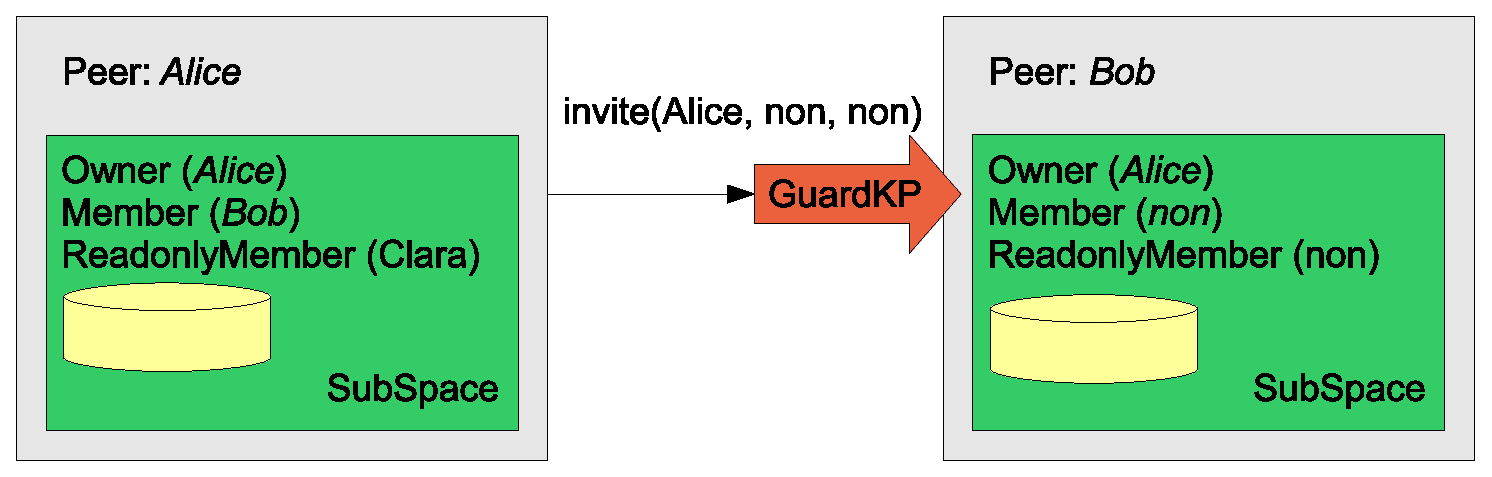
\includegraphics[width=0.60\textwidth]{subspaceAfterInvitation.eps}
\caption{Peers invited but not subscribed}
\label{fig:subspaceAfterInvitation}
\end{figure}

Figure \ref{fig:subspaceAfterInvitation} illustrates that situation.
Alice has invited Bob (beside Clara which isn't shown in th figure). The 
SubSpaceGuardKP has created the sub space in the Bob peer. Have a look
at the member lists. Only {\it Alice} as owner is known subspace because member.

Bob has two options: He can subscribe to the subspace or not. He hasn't to inform Alice if he doesn't want to enter the subspace. He can just remove the subspace from its system and is done.

Subscribing is pretty easy:

\begin{verbatim}
SubSpace aliceSubSpace = ...;
aliceSubSpace.subscribe();
\end{verbatim}

Actually two things happen: Alice gets informed that Bob has joined the subspace. Furthermore, a {\verb|SubSpaceKP|} is created that handles communication with other (subscribed) peers of the subspace.

Figure \ref{fig:subSpaceRefreshing} illustrates action which are and can
be performed afterwards. Alice has already received Bobs' subscription message. 
Thus, subspace status has changed: Bob became subscribed member. Alice refreshes
Claras list of members. Clara subscribes as well in our example. That message
is performed by Alice as well and leads to a refreshing message to Bob.

\begin{figure}[t]
\centering
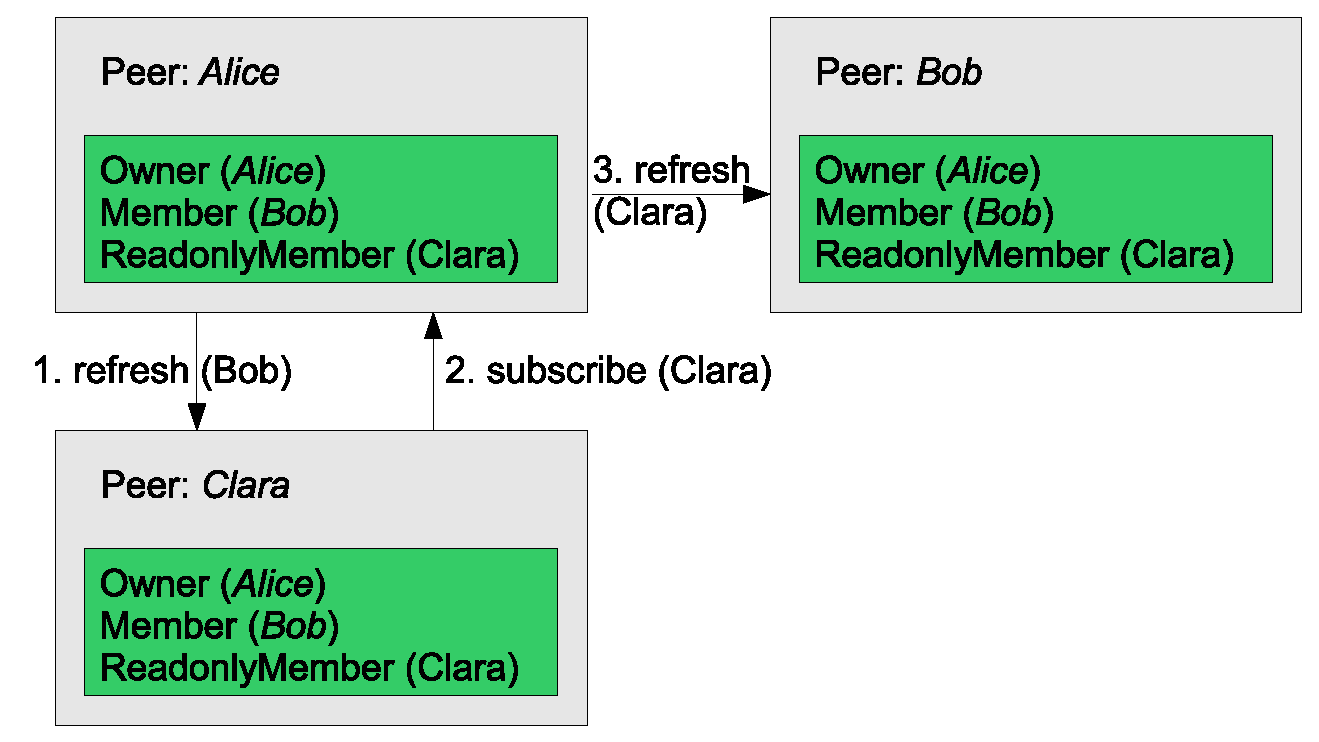
\includegraphics[width=0.60\textwidth]{subSpaceRefreshing.eps}
\caption{Refreshing subscription lists}
\label{fig:subSpaceRefreshing}
\end{figure}

Finally, any member has got the current subscription list.

The same procedure is performed when peers unsubscribe. An unsubscribe method changes member list in the owner which are propagated to all subspace members.

\subsection{Information exchange}
Member can add information to a subspace at any time. The data model doesn't differ from what we have already discussed until now. Peers can create context points and add information.

Subspaces differ in two ways: 

\begin{itemize}
\item 
Each locally added context point is sent
to each subscribed member.
\item 
Read only member are not allowed to add information into subspace knowledge
base. And attempt is answered with an exception.
\end{itemize}

Context point can be created with the subspace by using {\verb|createCP()|}. 
Information can be added now. The subspace automatically transmits any 
information that is added to all other subscribed peers.

Figure \ref{fig:subspaceAddingCP} illustrates this behaviour. The real user Alice adds information to her software. The Shark application uses a subspace for information storage and dissemination. Added information is stored locally in the Alice peer and also transmitted to any subscribed peer.

There is a callback method ({\verb|cpReached()|}) which is called when new
information has reached the subspace. Application can overwrite this method
what makes sense in most scenarios. Subspaces are e.g. used to implements 
chat rooms. A text or document is added in one peer and automatically 
distributed to others. The first peer is aware of new information due to
the performed user interaction. The other peer received those information
automatically via Shark. Their user interface needs to be informed to 
get refreshed. Use ({\verb|cpReached()|}) for such purposes.

This behaviour has implications:

\begin{itemize}
\item 
Only subscribed peer received added information. Thus, a peer doesn't get
automatically any information that was stored in the subspace. It only gets
information which are added after successful subscription.

\item 
Removing of information is not propagated. There are (yet) no means to inform
other peers about local deletion of information or whole context points.

\end{itemize}

\begin{figure}[t]
\centering
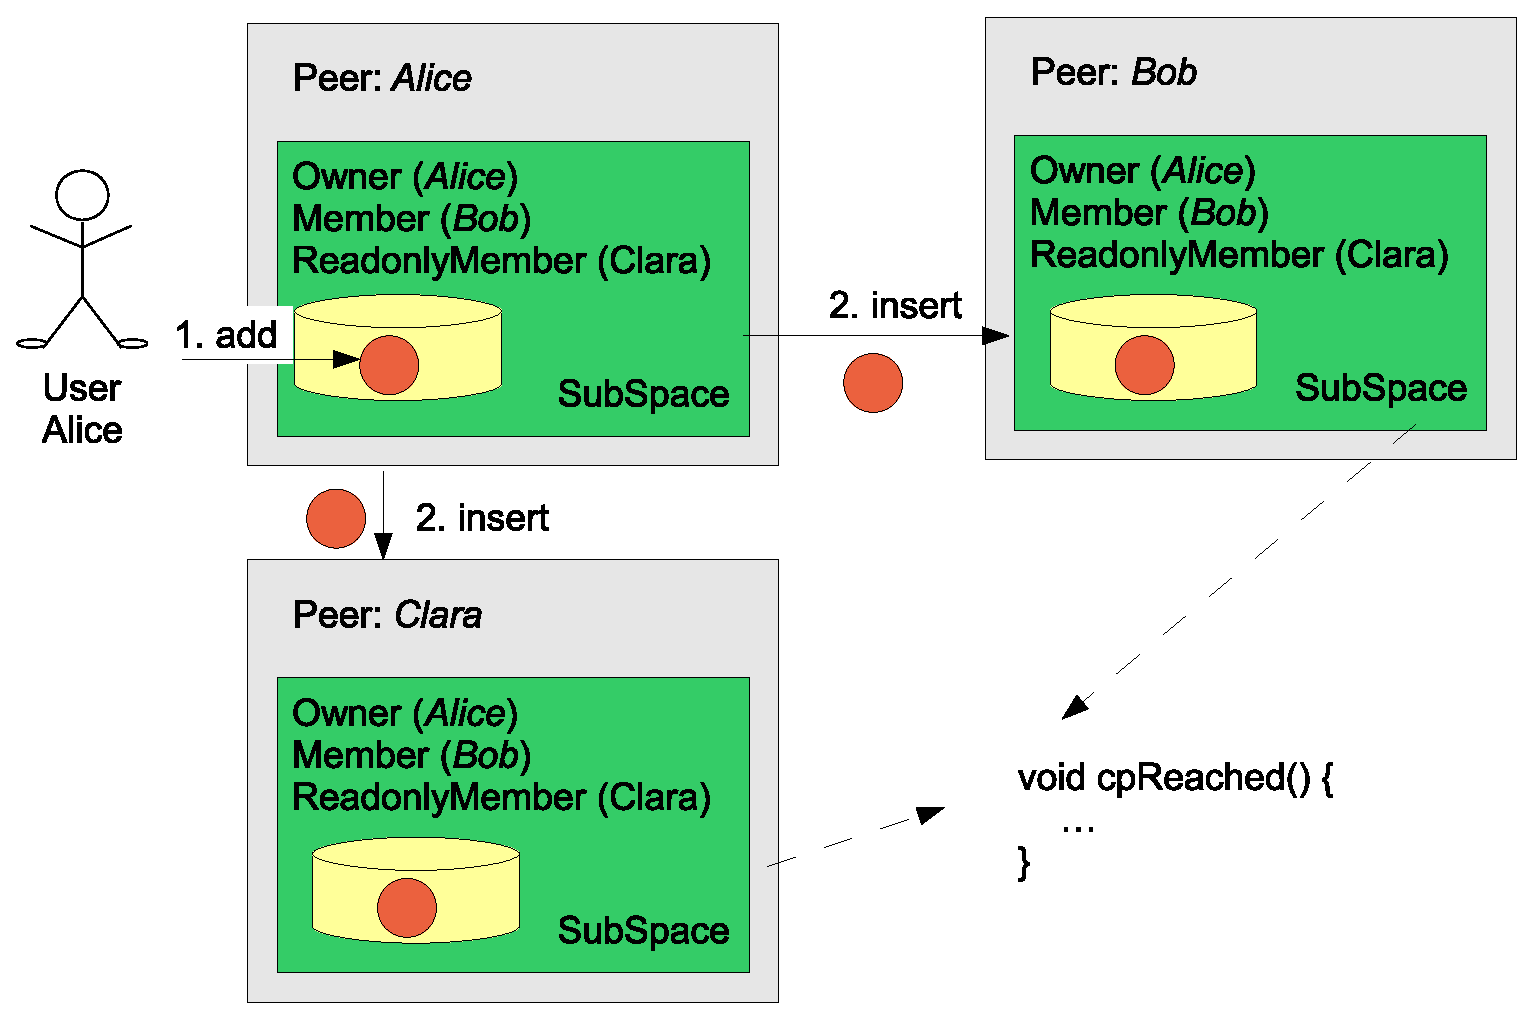
\includegraphics[width=0.60\textwidth]{subspaceAddingCP.eps}
\caption{Information synchronisation in sub spaces}
\label{fig:subspaceAddingCP}
\end{figure}

\subsection{Subspace knowledge base}

\section{Implementation details}
\subsection{Subspace Guard}
\subsection{Subspace KP}
\section{Implementing you own sub space}
\section{Using subspaces}

\section{Child sub spaces}

\section{Sub spaces usages}
\subsection{Chat}
\subsection{Makan}
\subsection{Forum}
\subsection{Shark Longitude}

%\chapter{Shark 3.0}
Shark is an open source project that is driven by a little team at a university with partners who work on actual applications. Have a look at www.sharksystem.net for more information.

Shark is used in projects. Each project has additional needs and requires additional functionality. Sometimes new custom functionality is worth to become a general framework function.

We have already identified two major enhancement which will be part of Shark 3.0.


\section{Public key infrastructure (PKI)}
Shark will get its own PKI. It already runs in our lab but wasn't tested enough to publish it. The general idea shall already be outlined, though.

Each peer will be able to create its own RSA key pair and then send its private key to another peer. The preferred way of public key exchange will be an ad-hoc network. Both persons see each others eyes and exchange key with their mobile phones.
Both can verify keys by fingerprints.

Keys can also be exchanged over larger distances by using other protocols. A fingerprint check is essential to ensure adding the right key.

Shark introduced the {\it trust level} which represents the number of peers that are between the key originator and the actual peer. A little example should illustrate the idea:

Alice creates a key pair and sends her public key directly to Bob. Of course, Bob has made all necessary fingerprint checks. Bob did not give Alice his public key. This key has actually the trust level 0. There is no peer between the originator Alice and the recipient Bob.

Imagine, Bob has already exchanged public keys with Clara. Their exchanged keys have the trust level 0 as well. Now, Bob might send Alice the public key of Clara. Clara would now have a public key of Alice, that was mediated by Bob. For Clara, the Alice key has the trust level 1 -- A single peer (Bob) mediated the key. Clara could send Alice's key to e.g. Daniel. He would have Alice's key with a trust level of two and so forth.

With that PKI, developers can define a minimum trust level which must be satisfied with peers to communicate. There might be applications who only accept a trust level 0 communication which means that each peer must know every other peer more or less personal. Of course, less secure applications will still be possible.

\section{Subspace}
Shark supports only peer-to-peer communication which is not very surprising for a P2P system. Most distributed applications require a communication between a closed group of peers. Social networks are a good example.

There can be groups exchanging information in a chat or with a variant of drop box. SharkNet is such an application. It comes with a chat and a concept called {\it makan}\footnote{Makan means room in Arabic.} which has features of a drop box -- it allows exchanging documents in a closed user group.

Still, there is no server involved. Any information is exchanged between all peers. It requires a special kind of protocol to create such chats and makan. Furthermore, it requires additional communication to introduce peers to those makan, to subscribe, unsubscribe and to remove it.

Shark 3.0 will introduce a concept called {\it subspace} which provides methods for creating many different kinds of such cooperative work. The concept is pretty simple: A peer creates a new knowledge base which is the new {\it subspace}.
A subspace comprises semantic tags and knowledge as usual.

The peer can introduces others to that subspace, though. Once a peer accepts an invitation it starts {\it sharing} the subspace. The result is pretty simple: Each new subscriber gets a copy of the subspace. Every subscriber is informed about the new subscriber. A subspace can have full subscribers and read-only subscribers. Full subscribers can also add information to the subspace. They simply add information with a context point.

The subspace automatically sends this new information to all subscribers. Note: There is no central entity. Any new information is submitted by the originator to every subscriber.

Peers can unsubscribe which actually means that all other subscribers get informed that this peer isn't interested in that subspace any more.

A subspace has similarities with an intranet application but there is no central instance. Each peer holds his own copy.

Of course, their can be a hierarchy of visibility rights which is achieved by structuring subspace memberships accordingly. We will explain that concept in the next version of this documentation. We can just state: The subspace concept was created to substitute parts of an internal intranet application. Thus, it meets all requirements of professional and commercial information exchange with the whole security and privacy background which is state of the art in the 21. century.

\section{.. and beyond: Shark Longitude}
There are also plans to implement Shark Longitude (SL) which will mainly focus on Android phones.

SL will provide users to get their own GPS coordinates which is pretty simple with Android. SL will also help creating tracks. More important, SL will allow sharing those information with other peers. Finally, a group of peers will share points of interests, tracks and current positions of others. There are well-know
applications having similar features. However, Shark Longitude makes it in a P2P manner: There is no server keeping all trails and points of any user. There is no need to trust a server that keeps personal trails which constitute highly sensitive data in most cases.

SL synchronises this data in a group of peers. They have to trust each other and nobody else.

Locations will be defined with Spatial Semantic Tags. We will introduce a very light version of a GIS into the systems. There will be a SL viewer of course which will be a mashup of the server based OSM data and the private P2P Shark data stored locally in the phones.

We cannot ensure that it will be already part of Shark 3.0. You are welcome to support these plans. Contact us!


%\bibliographystyle{alphadin}
%\bibliography{../../../../../../literatur}
\end{document}
